% 
% DESIGN DOCUMENT 
% ===============
% 
% Time-stamp: <2009-11-23 00:24:26 raskolnikov>
% (c) 2009 The JAGSAT development team.
% 

\documentclass[12pt,a4paper]{article}

\usepackage{raskolnikov}

\title{\large JAGSAT project\\\huge Design Document}
\author{
  Juan Pedro Bolívar Puente\\ 
  Aksel Junkkila\\
  Guillem Medina\\ 
  Sarah Lindstrom\\ 
  Alberto Villegas Erce\\ 
  Thomas Forss
}
\location{Project Course \\ \textit{Åbo Akademy}}

\let\stdsection\section
\renewcommand\section{\newpage\stdsection}

\disabletodo

\begin{document}
\maketitle

\begin{center}
\textbf {Revision history}

\begin{tabular}{ l | l | l | l }
Date			&Version	&Description			&Author\\\hline\hline
01.10.2009	&0.1		&Design document		&Thomas Forss\\
10.10.2009	&0.2		&Use cases			&Thomas Forss\\
20.10.2009	&0.3		&Added user Interface	&Juan Pedro Bolívar\\
30.10.2009	&0.3		&Added state diagrams	&Juan Pedro Bolívar\\
10.12.2009	&1.0		&Delivery editing 		&Alberto Villegas\\
22.03.2010	&2.0		&Reviewed			&Alberto Villegas
\end{tabular}
\label{tab:rev}
\end{center}

\vfill
Copyright 2009 AUTHORS.
Permission is granted to copy, distribute and/or modify this document under the terms of the GNU Free Documentation License, Version 1.1 or any later version published by the Free Software Foundation;  with no Invariant Sections, with no Front-Cover Texts, and with no Back-Cover Texts. A copy of the license is included in the ``D9: Licenses''  document entitled `GNU Free Documentation License''.

\pagebreak
\tableofcontents
\pagebreak

\section{Introduction}

The aim of this document is multiple, on one hand is a way to establish 
communication gates between our client and us, showing what and how
we plan to do as a matter of contract. On the other hand is a guide to
follow by our developers, well defined steps and rules of what our
client wants to be done.
 
In the following pages there will be found several descriptions about 
interfaces, use cases, rules and design of the project. Due to the nature of 
the project there will probably be some inconsistencies between this
document and the final released product. As a game itself, its design
relies on the playability which, in any case, can only be measured
empirically through a process of testing and continuous elliptical
modifications and refining.

\section{Game design}

\subsection{Introduction}

This section describes the overall game design. Firstly a detailed view
of the game rules, in both parts of the game. These rules describe what
players will be able to do and not to do. Secondly an overview of the
user interface which, in any case, is deeply detailed and illustrated in
section 7. Thirdly, and finally, a detailed list of the graphics and 
animations that will be needed in the final version.

\begin{todo}[Juan Pedro]
  While reading the whole text during the refactor we have found
  important inconsistencies. The Axel description of the rules and
  interface does not match very well with my state machines and the UI
  diagrams. Also, some parts of it are too schematic and hard to
  understand that could be improved with longer descriptions and
  better ordering of some items. Also, the list of graphics needed for
  the project is too long, there are many things that are not needed
  (afaik) or clear. For example, we don't need unit pictures for the
  world map, because it much more reasonable to use numbers to
  represent the number of units.
\end{todo}

\subsection{World Domination}

\subsubsection{General rules}

\begin{todo}[Juan Pedro]
  There are some misunderstandings in the rules. Maybe we can copy paste
  from the Wikipedia page (be careful with the license, but probably
  there is no problem on making this doc GFDL, actually the
  \texttt{.doc} version was...):
  \url{www.wikipedia.org/wiki/Risk_(game)}
\end{todo}

\begin{itemize}
\item Every player has an objective, the objectives are determined by
  drawing cards.
\item World map is divided into countries, every player gets countries
  on random.
\item Every player gets troops and deploy them in their countries.
\item The world domination game is played in turns.
\item Starting player is chosen by random.
\item Player turn order is clockwise.
\end{itemize}

\subsubsection{During turn}

\begin{itemize}
\item There are 3 phases in a players turn. Reinforcements, attacking
  and moving.
\item Reinforcement troops are obtained at the beginning of the turn. 
  The player obtains 1/3 of his/her number of countries units with a minimum 
  of three.
\item The player receives additional units based on continents.
\item The player may also receive units if he turns in a set of unit
  cards. He then places the units on any of his territories.
\item If the player has conquered at least one territory, he draws a
  unit card from the deck. 
\item A set of unit cards consists of one of the following:
  \begin{itemize}
  \item Three cards depicting the same unit (eg. all three cards have
    infantry pictures)
  \item Three cards showing one of each type of Risk unit (infantry,
    barrier, cannon).
  \end{itemize}
\item A country must always have one unit in it.
\item A unit in a country can only move to a neighbor country.
\item A player can attack nearby countries from the country he owns.
\item A player must have more than one unit in a country to be able to
  attack another country.
\item When a player attacks he attacks with a chosen number of units,
  between 1 to 3, from the attacking country.
\item The defender defends with a chosen number of units, one or two,
  from the defending country.
\item A conquered country cannot attack nearby countries within the
  same turn it gets conquered.
\item Units can only attack once every turn.
\item A unit is considered used when it destroys an enemy unit or is
  moved in the moving phase.
\item Units can be moved between owned neighbor countries if they 
  have not been used before.
\end{itemize}

\subsection{Tower defense}

\subsubsection{General rules}
\begin{itemize}
\item Tower defense gameplay is live.
\item Tower defense battlefield is divided into 4 zones consisting of
  a defending zone and an middle zone for both players. This means
  both players have an area to defend and a middle area to maneuver
  in.
\item The attacker and defender both get 3 different kind of
  units. These are cannons, infantry and barriers.
\item There is an option of surrendering, the time when you can
  surrender is determined randomly. The timelimit for surrendering is
  10 seconds. Exception: You can not surrender in the beginning.
\item There is a time limit to a battle. If the winner has not been
  determined by that point the battle will be considered a tie and the
  units lost will be registered.
\item There is the option to choose the speed of the battle
  game. \emph{Optional}.
\end{itemize}

\subsubsection{The set up}
\begin{itemize}
\item Setting up units will be live. A player can choose when to place
  his units on the field.
\item Before the battle begins, the defender will flip a coin. For
  every right coinflip he will get one more unit up to a maximum of
  the attackers amount of units. If the attacker has less units than
  the defender there will be no coinflip.
\item Attacker gets infantry, cannons and barriers equaling to the
  amount of units he his attacking with. If the attacker is attacking
  with 5 units he will get 5 of each.
\item The defender gets infantry, cannons and barriers equaling to the
  amount of units he is defending with.
\item The defender also has the chance on getting extra units, this
  will be determined randomly. The defenders extra units will not
  count as units on world map.
\item Cannons can be set up at defense zone only. Their placement will
  be random and the cannons will be stationary.
\item Infantry can be set up anywhere in the players own defending
  area or middle area.
\item Barriers can only be set up at players own middle area.
\end{itemize}

\subsubsection{Gameplay}
\begin{itemize}
\item Cannons can destroy barriers.
\item Cannons can also destroy enemy cannons.
\item Barriers can block infantry. A blocked infantry dies.
\item Infantries are equal and destroy each other if they meet.
\item Infantry can pass the defense line. An infantry passing the defense
  line will kill an enemy unit on the world map. Thus if enough
  infantry pass the line the country gets conquered.
\item Infantry can bounce from battlefield edges. 
\item Cannonballs do not bounce but disappear if they are shot out of
  the battlefield area.
\end{itemize}

\begin{figure}[h!]
\centering
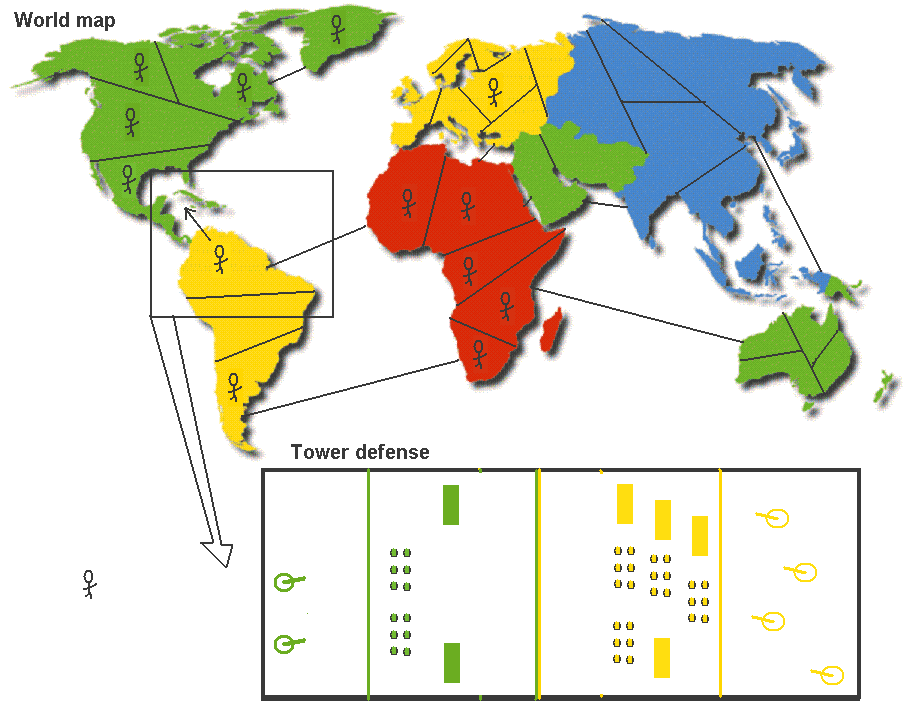
\includegraphics[width=13cm]{pic/rules.png}
\caption{Mockup of the game play interface.}
\label{fig:gameplay}
\end{figure}

\subsection{Interface}

\subsubsection{World map}

\begin{itemize}
\item Every player has a personal menu button that shows player 
  options: next, undo, objectives and cards.
\item Objective cards are shown when clicking on the objective button.
\item Cards are shown when clicking on the card button.
\item Player passes to next phase when clicking on the next button.
\item Player undo his last action by clicking on the undo button.
\item In the deployment and reinforcement phase. A player can deploy
  his units by clicking repetitively on a country, as many times as units
  he want to place.
\item A player can move units from one country to another by clicking
  on a country he wants to move units from. Then the neighbor owned
  countries are highlighted. By clicking the source country, units are 
  stored on a counter waiting for a neighbor country click to move.
\item Attacking a country is done by clicking on an own country and
  then clicking a neighbor enemy country.
\end{itemize}

\subsubsection{Tower defense}
\begin{itemize}
\item A player can set up infantry anywhere on his own zones. He will
  do so by clicking on a infantry icon and then clicking on a spot on
  one of his zones. After the infantry has been deployed he steers the
  infantry in a direction by clicking on the screen. An arrow will
  point the direction.
\item A player can set up barriers anywhere on his own middle zone. He
  will do so by clicking on the barrier icon and then clicking again
  on a spot that he wants to block. The barrier is now set and can not
  be moved again.
\item Cannon placement is randomized within the defense zone. A player
  can choose a cannon by clicking on it. When he chooses a cannon an
  arrow appears, he can steer the arrow in a direction by dragging
  with his finger on the display. The more he drags the longer will
  the shot be.
\item A player can alter the movement of his infantries while they are
  within his own middle zone. He will do so by clicking on a infantry
  unit and an arrow appears. He will choose the new direction by
  clicking on the screen again.
\item A currently chosen unit will be highlighted.
\item When the surrender time option is available a surrender button
  will appear for both players. If a player clicks on the button he
  will surrender. When surrender time is over the button disappears.
\item Before the actual battle begins the defender flips a coin for
  more units. He will do so by choosing heads or tails and a
  randomizer will show the result.
\end{itemize}

\subsection{Graphics}

\subsubsection{Main Intro. \emph{optional}}

\subsubsection{Main screen}
\begin{itemize}
\item Main game menu
\item New game options screen
\item Number of players.
\item Different colors for player characters
\item Player position
\item Player name
\item Sound menu
\end{itemize}

\subsubsection{Main Map}
\begin{itemize}
\item Divided in areas
\item Even and squared or uneven areas
\item Player name whose turn it is, is shown 
\item Turn number shown/ Year or equivalent
\item Player controlled areas shown
\item Different colors for each players
\item Player units shown
\item Attack screen/ animation shown when attacking.
\end{itemize}

\subsubsection{Battlefields}
\begin{itemize}
\item Different backgrounds depending on country/area
\item Forrest
\item Size of battlefield always same
\item Bridges
\item Water / Rivers
\item Rocks
\item Generating random battlefields. \emph{Optional}.
\item Time limit shown
\item Roles, the defender and the attacker shown
\item Defending and middle zones shown
\end{itemize}

\subsubsection{Units}

\subsubsection{Main Map Units}
\begin{itemize}
\item Player units
\item Shown in a way so that all players can see everyones units
\item Battlefield Units
\item Troops
\item Health shown. \emph{Optional}.
\item Cannons
\item Health shown. \emph{Optional}.
\item Barriers
\item Health shown. \emph{Optional}.
\end{itemize}

\subsubsection{Animations}

\begin{itemize}
\item Troop animations: \emph{Movement, Shooting, Death}
\item Cannon animations: \emph{Movement, Shooting, Death}
\item Barrier animations: \emph{Placement (Optional), blocking
    infantry, Destroyed by cannon}
\item Player unit movement on main map
\item Area highlighting when chosen
\item A players battlefield unit currently in control is shown somehow
\item Highlighted, with the specific player color
\item Going into battlefield animation \emph{optional}.
\item Attack animation on main map \emph{optional}.
\end{itemize}

% \twocolumn

\section{Use cases}

\subsection{Start Game}
\begin{description}
\item[Priority] 1
\item[Users] User, game.
\item[Precondition] None.
\item[Flow]\mbox{}
  \begin{enumerate}
  \item Users open game.
  \item Game plays a short clip.
  \item Game menu initiates.
  \end{enumerate}
\item[Postcondition] Program is running.
\item[Alternative Flow 1]\mbox{}
  \begin{enumerate}
  \item User opens game.
  \item Game menu initiates.
  \end{enumerate}
\end{description}

\subsection{Player settings}
\begin{description}
\item[Priority] 3
\item[Users] User, game
\item[Precondition] Game is initiated.
\item[Flow]\mbox{}
  \begin{enumerate}
  \item Player chooses \emph{New Game} in menu.
  \item User chooses amount of players.
  \item User enter new names.
  \end{enumerate}
\item[Postcondition] None.
\item[Alternative Flow 1]\mbox{}
  \begin{enumerate}
  \item User chooses amount of players.
  \item User chooses default names.
  \end{enumerate}
\item[Alternative Flow 2]\mbox{}
  \begin{enumerate}
  \item User goes back to menu.
  \end{enumerate}
\end{description}

\subsection{Game settings}
\begin{description}
\item[Priority] 3
\item[Users] User, game
\item[Precondition] Amount of players set.
\item[Flow]\mbox{}
  \begin{enumerate}
  \item User chooses a map from the list.
  \item Game starts.
  \end{enumerate}
\item[Postcondition] Game starts.
\item[Alternative Flow 1]\mbox{}
  \begin{enumerate}
  \item User goes back to edit player settings.
  \end{enumerate}
\end{description}

\begin{todo}[Juan Pedro]
  Choosing the game length might be no longer needed because we now let
  the user choose an arbitrary map from the list?
\end{todo}

\subsection{Sound settings}
\begin{description}
\item[Priority] 4
\item[Users] User, game
\item[Precondition] Game menu is initialized.
\item[Flow]\mbox{}
  \begin{enumerate}
  \item User chooses \emph{Sound settings} from menu.
  \item User changes sound settings.
  \item User saves changes.
  \end{enumerate}
\item[Postcondition] Settings are changes. 
\item[Alternative Flow 1]\mbox{}
  \begin{enumerate}
  \item User chooses \emph{Sound settings} from menu.
  \item User discards changes.
  \end{enumerate}
\end{description}

\subsection{Player takes turn}

\begin{description}
\item[Priority] 1
\item[Users] User, game
\item[Precondition] Game has started.
\item[Flow]\mbox{}
  \begin{enumerate}
  \item Player places reinforcements on field.
  \item Player attacks enemy countries.
    \begin{enumerate}
    \item Tower defense starts.
    \item Tower defense ends.
    \end{enumerate}
  \item Player moves troops.
  \item User ends turn.
  \end{enumerate}
\item[Postcondition] Turn is over.
  % \item[Alternative Flow 1]\mbox{}
  %   \begin{enumerate}
  %   \item 
  %   \end{enumerate}
\end{description}

\subsection{Attacker (Tower defense)}

\begin{description}
\item[Priority] 3
\item[Users]  User, game.
\item[Precondition] Player attacks enemy area.
\item[Flow]\mbox{}
  \begin{enumerate}
  \item Amount of units in area are converted into money.
  \item User chooses what units to build.
  \item Player places units on field.
  \item Player passes enough units onto enemy area.
  \item User takes control of area.
  \item All units but one moves into new area.
  \end{enumerate}
\item[Postcondition] None.
\item[Alternative Flow 1]\mbox{}
  \begin{enumerate}
  \item Player chooses what units to build.
  \item Player places units on field.
  \item Player runs out of money.
  \item Player fails to pass enough units to enemy area.
  \item Player does not take control of area.
  \end{enumerate}
\item[Alternative Flow 1]\mbox{}
  \begin{enumerate}
  \item Player chooses what units to build.
  \item Player places units on field.
  \item Player runs out of time.
  \item Player does not take control of area.
  \end{enumerate}
\end{description}

\begin{todo}[Juan Pedro]
  This use-case does not reflect the game rules. One does not have money
  anymore, and the defender can actually takeover the attacker country.
\end{todo}

\subsection{Defender (Tower defense)}
\begin{description}
\item[Priority] 3
\item[Users]  User, game
\item[Precondition]  User attacks enemy area.
\item[Flow]\mbox{}
  \begin{enumerate}
  \item Amount of units are converted into money.
  \item Player chooses what units to build.
  \item Player places units on field.
  \item Attacker fails to pass enough units.
  \item User defends area.
  \item User keeps control of area.
  \end{enumerate}
\item[Postcondition] None.
\item[Alternative Flow 1]\mbox{}
  \begin{enumerate}
  \item Player chooses what units to build.
  \item Player passes enough units to attackers side.
  \item Player keeps control of area.
  \end{enumerate}
\item[Alternative Flow 2]\mbox{}
  \begin{enumerate}
  \item Player chooses what units to build
  \item Player runs out of money.
  \item Attacker fails to pass enough units.
  \item Player keeps control of area.
  \end{enumerate}
\item[Alternative Flow 3]\mbox{}
  \begin{enumerate}
  \item Player chooses what units to build.
  \item Player runs out of time.
  \item Player keeps control of area.
  \end{enumerate}
\end{description}

\subsection{Player is eliminated}
\begin{description}
\item[Priority] 2
\item[Users] User, game.
\item[Precondition] Game has started.
\item[Flow]\mbox{}
  \begin{enumerate}
  \item Player loses last area.
  \item Player is removed from turn list.
  \item Losing sound is player.
  \end{enumerate}
\item[Postcondition] Player is out of the game.
  % \item[Alternative Flow 1]\mbox{}
  %   \begin{enumerate}
  %   \item 
  %   \end{enumerate}
\end{description}

\subsection{Player wins the game}
\begin{description}
\item[Priority] 2
\item[Users] User, game
\item[Precondition]  Game has started.
\item[Flow]\mbox{}
  \begin{enumerate}
  \item Player accomplish his mission.
  \item All other users are removed from turn list.
  \item Winning sound is played.
  \item Game statistics are showed.
  \end{enumerate}
\item[Postcondition] Game is over.
\item[Alternative Flow 1]\mbox{}
  % \begin{enumerate}
  % \item 
  % \end{enumerate}
\end{description}

\subsection{Save game}
\begin{description}
\item[Priority] 4
\item[Users] User, game.
\item[Precondition] Game is active.
\item[Flow]\mbox{}
  \begin{enumerate}
  \item User choose \emph{Save and quit game}.
  \item User specifies save game.
  \end{enumerate}
\item[Postcondition]  Game ends.
  % \item[Alternative Flow 1]\mbox{}
  %   \begin{enumerate}
  %   \item 
  %   \end{enumerate}
\end{description}

\subsection{Load game}
\begin{description}
\item[Priority] 4
\item[Users] User, game.
\item[Precondition] Program is open.
\item[Flow]\mbox{}
  \begin{enumerate}
  \item Users chooses \emph{Load game}.
  \item User specifies load game.
  \end{enumerate}
\item[Postcondition] Game re-initiated.
  % \item[Alternative Flow 1]\mbox{}
  %   \begin{enumerate}
  %   \item 
  %   \end{enumerate}
\end{description}

\subsection{Game start (World domination)}
\begin{description}
\item[Priority] 1
\item[Users] User, game.
\item[Precondition] None.
\item[Flow]\mbox{}
  \begin{enumerate}
  \item Each player is given an objective.
  \item World map is divided on random.
  \item Each player deploys troops depending on country size.
  \item Starting player is chosen by random.
  \item Players take turn in clockwise order.
  \end{enumerate}
\item[Postcondition] None.
  % \item[Alternative Flow 1]\mbox{}
  %   \begin{enumerate}
  %   \item 
  %   \end{enumerate}
\end{description}

\subsection{Reinforcements (World domination)}
\begin{description}
\item[Priority] 2
\item[Users] User, game.
\item[Precondition] Player takes turn.
\item[Flow]\mbox{}
  \begin{enumerate}
  \item Player receives 1 reinforcements for each 3 countries he owns.
  \item Player receives reinforcements for continents controlled.
  \item Player places reinforcements on the game board.
  \end{enumerate}
\item[Postcondition] None.
\item[Alternative Flow 1]\mbox{}
  \begin{enumerate}
  \item Player has 3 conquer cards of the same type.
  \item Player receives 1 troop at next reinforcement.
  \end{enumerate}
\item[Alternative Flow 2]\mbox{}
  \begin{enumerate}
  \item Player has 3 conquer cards of different type.
  \item Player receives 2 troop at next reinforcement.
  \end{enumerate}
\end{description}

\begin{todo}[Juan Pedro]
  The reinforcements are actually given in a different way. The cards
  are exchanged in any moment during the user reinforcement phase (at
  user will, he can keep them for later use also) and the values that he
  gets for it are different.
\end{todo}

\subsection{Attack (World domination)}
\begin{description}
\item[Priority] 2
\item[Users] User, game.
\item[Precondition] Player controls at least 2 units in area and
  player takes turn.
\item[Flow]\mbox{}
  \begin{enumerate}
  \item Player marks a country that has at least two unused units.
  \item Player selects neighbouring enemy country to attack.
  \item Dices are thrown 
  \end{enumerate}
\item[Alternative Flow 1]\mbox{}
  \begin{enumerate}
  \item Tower defense is initiated.
  \end{enumerate}
\item[Postcondition] None.
  % \item[Alternative Flow 1]\mbox{}
  %   \begin{enumerate}
  %   \item 
  %   \end{enumerate}
\end{description}

\subsection{Movement (World domination)}
\begin{description}
\item[Priority] 2
\item[Users] User, game.
\item[Precondition] Player takes turn.
\item[Flow]\mbox{}
  \begin{enumerate}
  \item Player selects number $\delta$ of troops in a country that have not moved
    this turn.
  \item Player selects neighbouring country controlled by the same
    player.
  \item Troops move.
  \end{enumerate}
\item[Postcondition] $\delta$ troops are moved from the source country
  to the target.
  % \item[Alternative Flow 1]\mbox{}
  %   \begin{enumerate}
  %   \item 
  %   \end{enumerate}
\end{description}

\subsection{Conquering country (World domination)}
\begin{description}
\item[Priority] 2
\item[Users] User, game.
\item[Precondition] Player takes turn.
\item[Flow]\mbox{}
  \begin{enumerate}
  \item Attacking player wins dices phase.
  \item All surviving units are moved to the conquered country.
  \item Player draws conquer card.
  \end{enumerate}
\item[Postcondition] None.
\item[Alternative Flow 1]\mbox{}
  \item Attacking player wins tower defense battle.
  \item All units except one move into conquered country.
  \item Player draws conquer card.
\item[Alternative Flow 2]\mbox{}
  \begin{enumerate}
  \item Defending player wins tower defense battle (no surviving
    attackers).
  \item One unit move into attackers country.
  \end{enumerate}
\end{description}

\begin{todo}[Juan Pedro]
  The defender should not draw a conquer card AFAIK. Also, the attacker
  gets the amount of troops used (that crossed the border) into the
  other country if he wins. In any case the troops that crossed the
  border are marked as used.
\end{todo}

\subsection{Retreat (Tower defense)}
\begin{description}
\item[Priority] 3
\item[Users] User, game.
\item[Precondition] Tower defense is initiated.
\item[Flow]\mbox{}
  \begin{enumerate}
  \item Attacking player uses retreat option.
  \item Tower defense is ended.
  \item Surviving attacking units go back to attackers country.
  \end{enumerate}
\item[Postcondition] None.
\item[Alternative Flow 1]\mbox{}
  \begin{enumerate}
  \item Defending player uses retreat option.
  \item Tower defense is ended.
  \item Attacking player conquers country.
  \item Surviving defending units move into closes country (random if several).
  \end{enumerate}
\end{description}

\subsection{Build (Tower defense)}
\begin{description}
\item[Priority] 3
\item[Users] User, game.
\item[Precondition] Tower defense initiated.
\item[Flow]\mbox{}
  \begin{enumerate}
  \item Player selects troops.
  \item Player selects location.
  \item Player selects angle.
  \item Player selects speed.
  \end{enumerate}
\item[Postcondition] None.
\item[Alternative Flow 1]\mbox{}
  \begin{enumerate}
  \item Player selects barrier.
  \item Player selects location.
  \item Player selects angle.
  \end{enumerate}
\end{description}

\subsection{Coin flip (Tower defense)}
\begin{description}
\item[Priority] 4
\item[Users] User, game.
\item[Precondition] Tower defense is initiated. Attacker has more
  units than defender.
\item[Flow]\mbox{}
  \begin{enumerate}
  \item Defending player flips coin.
  \item Coin flip successful.
  \item Virtual unit (only valid during this tower defense battle) added
    to defender.
  \item Repeat if attacker has more units.
  \end{enumerate}
\item[Postcondition] None.
\item[Alternative Flow 1]\mbox{}
  \begin{enumerate}
  \item Defending player flips coin.
  \item Coin flip fails. No more coin flips.
  \end{enumerate}
\end{description}

\subsection{Collision (Tower defense)}
\begin{description}
\item[Priority] 3
\item[Users] User, game
\item[Precondition] Tower defense is initiated.
\item[Flow]\mbox{}
  \begin{enumerate}
  \item Two troops from different team collide.
  \item Both troops die.
  \end{enumerate}
\item[Postcondition] None.
\item[Alternative Flow 1]\mbox{}
  \begin{enumerate}
  \item Troop collides with barrier.
  \item Troop bounces away at same angle as it entered.
  \end{enumerate}
\end{description}

\begin{todo}[Juan Pedro]
  I think that we agreed on Axel suggestion about troops not bouncing
  but just dying on collision with a barrier (can represent the unit
  being killed by the archers or something).
\end{todo}

\subsection{Shoot cannon (Tower defense)}
\begin{description}
\item[Priority] 3
\item[Users] User, game.
\item[Precondition] Tower defense is initiated.
\item[Flow]\mbox{}
  \begin{enumerate}
  \item Player selects cannon.
  \item Player selects angle.
  \item Player selects speed.
  \item Player presses shoot.
  \item Player hits barrier or cannon.
  \item Barrier or cannon is destroyed.
  \end{enumerate}
\item[Postcondition] None.
\item[Alternative Flow 1]\mbox{}
  \begin{enumerate}
  \item Player selects cannon.
  \item Player selects angle.
  \item Player selects speed.
  \item Player presses shoot.
  \item Player misses.
  \end{enumerate}
\end{description}

\subsection{Change direction (Tower defense)}
\begin{description}
\item[Priority] 4
\item[Users] User, game.
\item[Precondition] Tower defense is initiated.
\item[Flow]\mbox{}
  \begin{enumerate}
  \item Player selects a troop on his side of the field.
  \item Player changes direction.
  \item Unit changes direction.
  \end{enumerate}
\item[Postcondition] None.
\end{description}

\subsection{Used unit (Tower defense)}
\begin{description}
\item[Priority] 3
\item[Users] User, game.
\item[Precondition] Tower defense is initiated.
\item[Flow]\mbox{}
  \begin{enumerate}
  \item A unit passes enemy defenses in tower defense.
  \item The unit is marked as used.
  \item A unit is deducted form the opponents country units and
    considered \emph{dead}.
  \end{enumerate}
\item[Postcondition] None.
\end{description}

%%%% 
% \subsection{}
% \begin{description}
% \item[Priority]
% \item[Users] 
% \item[Precondition] 
% \item[Flow]\mbox{}
%   \begin{enumerate}
%   \item 
%   \end{enumerate}
% \item[Postcondition] 
% \item[Alternative Flow 1]\mbox{}
%   \begin{enumerate}
%   \item 
%   \end{enumerate}
% \end{description}

\onecolumn


\section{Class design}

\subsection{Introduction}
This section models the static design of the project using class
diagrams that provide a bird-sight view of the code structure based on
classes and their relationships.

\subsection{Global diagram}
\begin{figure}[H]
  \centering
  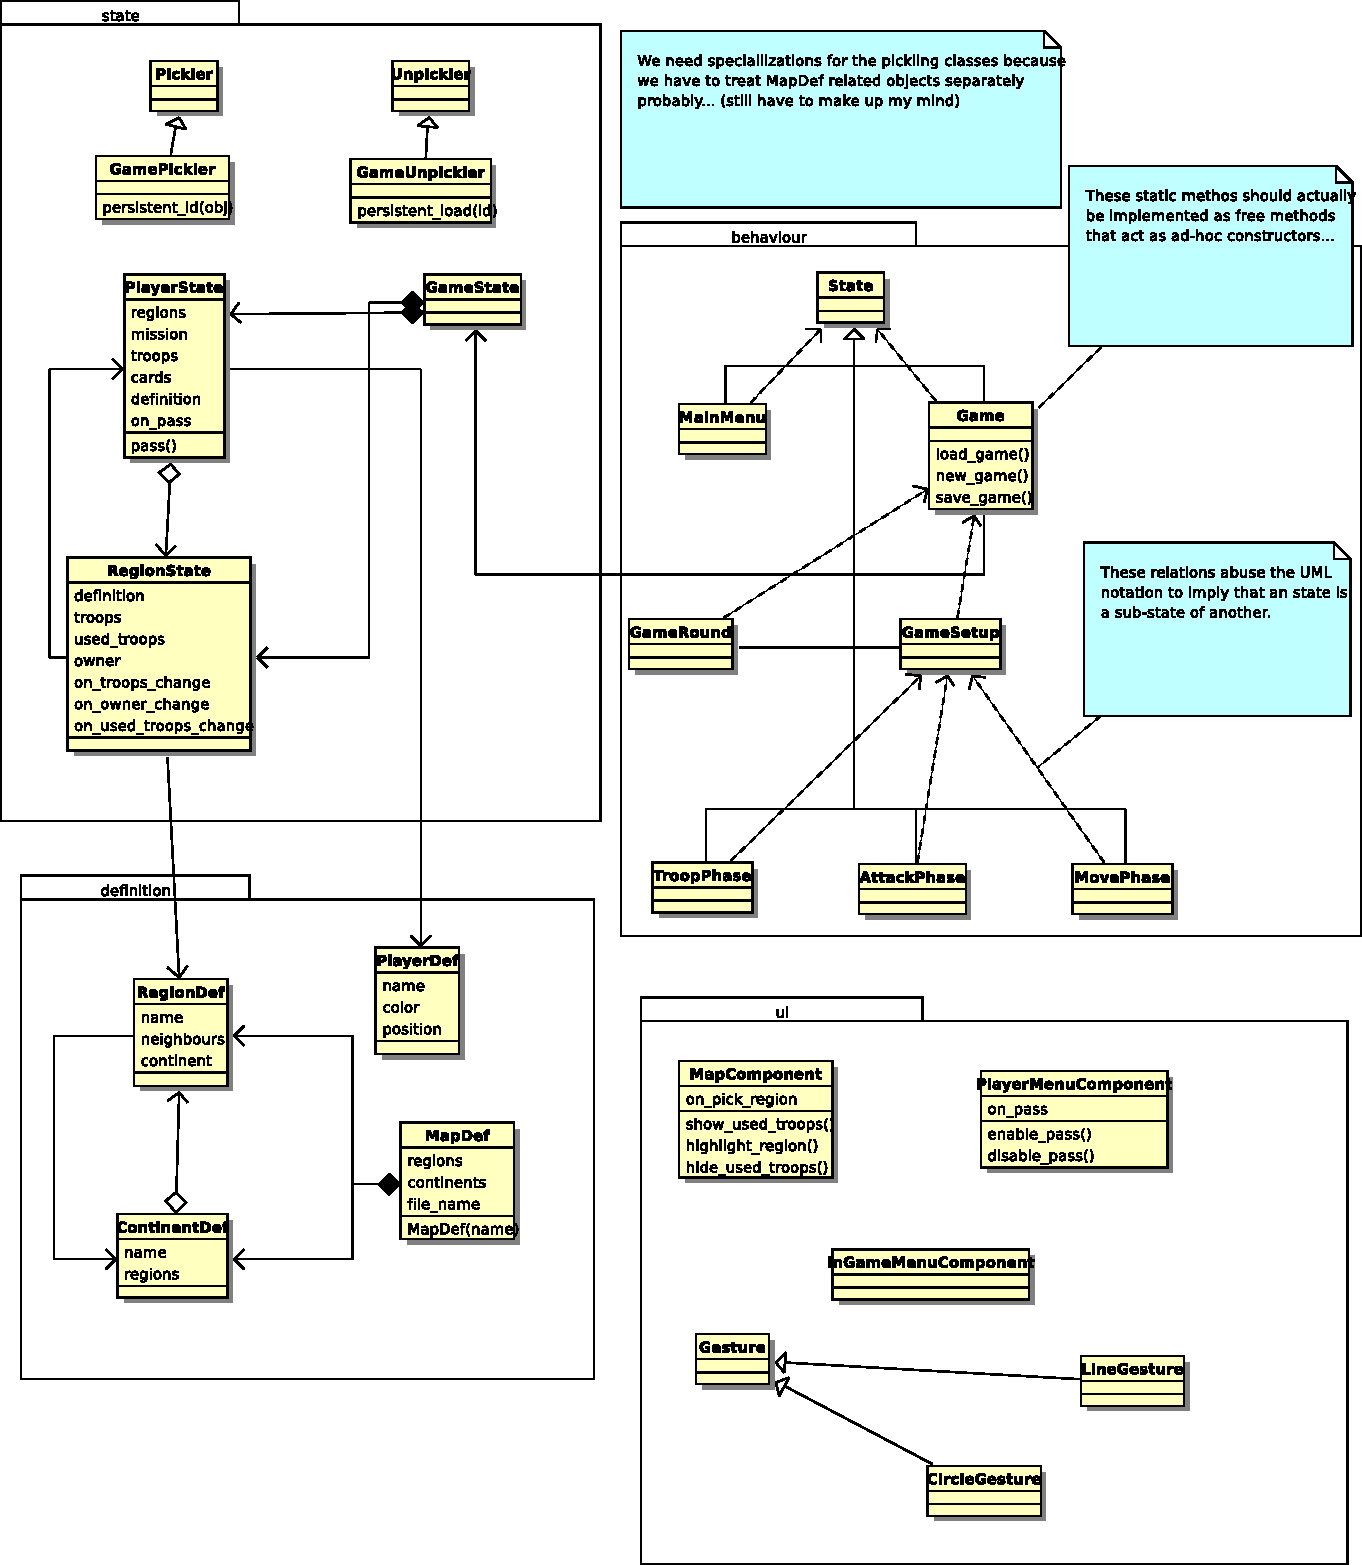
\includegraphics[width=14cm]{pic/8.pdf}
  \caption{Class diagram.}
  \label{fig:class}
\end{figure}

\begin{todo}[Juan Pedro]
  This diagram is not finished. But I must admit that I consider a bit
  pointless finishing it right now... Also, splitting it into multiple
  diagrams can be a good idea. Any suggestions?
\end{todo}

\section{State machines}

\begin{todo}
  Maybe some further description and connection to the use cases in
  the state diagrams would be good...
\end{todo}

\subsection{Introduction}
This section models the dynamic behaviour of the program using class
diagrams that model main interaction through events and states and the
actions associated to them.

\subsection{Global state machine}
\begin{figure}[h!]
  \centering
  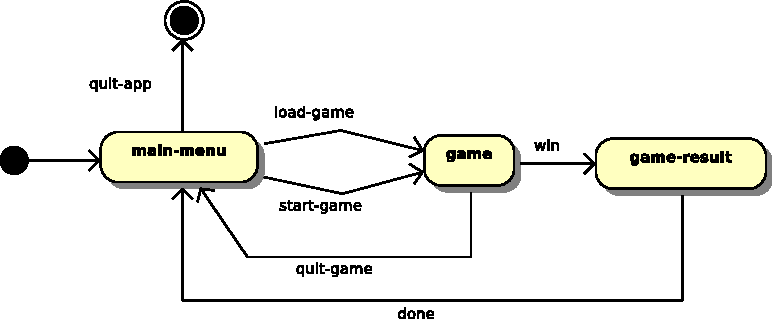
\includegraphics[width=13cm]{pic/1.pdf}
  \caption{Global state machine.}
  \label{fig:sm:global}
\end{figure}

\subsection{\texttt{game} state machine.}
\begin{figure}[H]
  \centering
  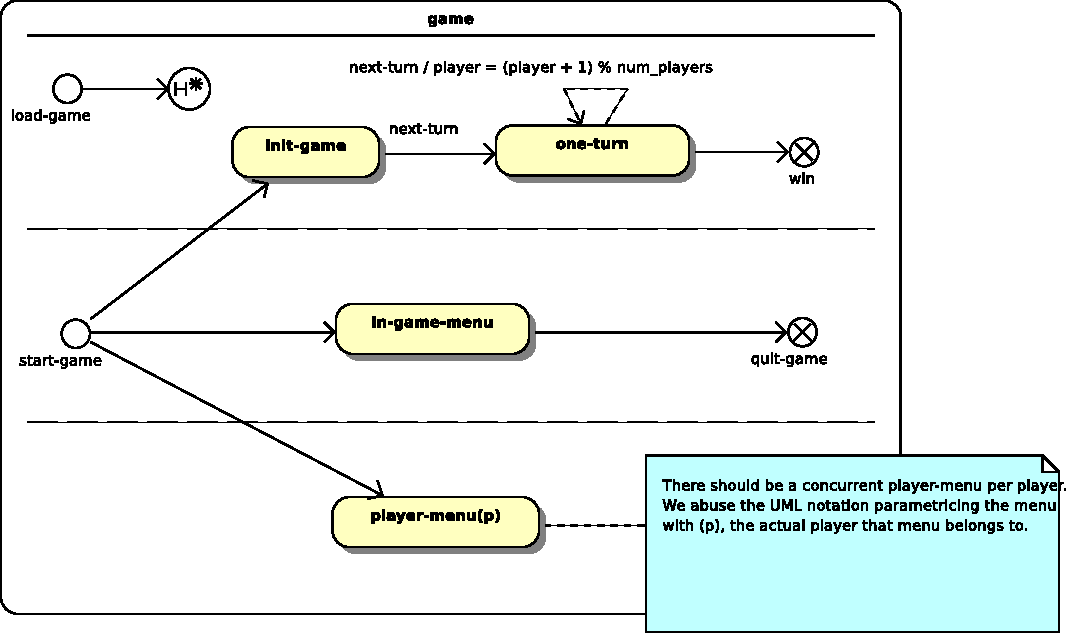
\includegraphics[width=15cm]{pic/2.pdf}
  \caption{\texttt{game} state machine.}
  \label{fig:sm:game}
\end{figure}

\subsection{\texttt{init-game} state machine.}
\begin{figure}[H]
  \centering
  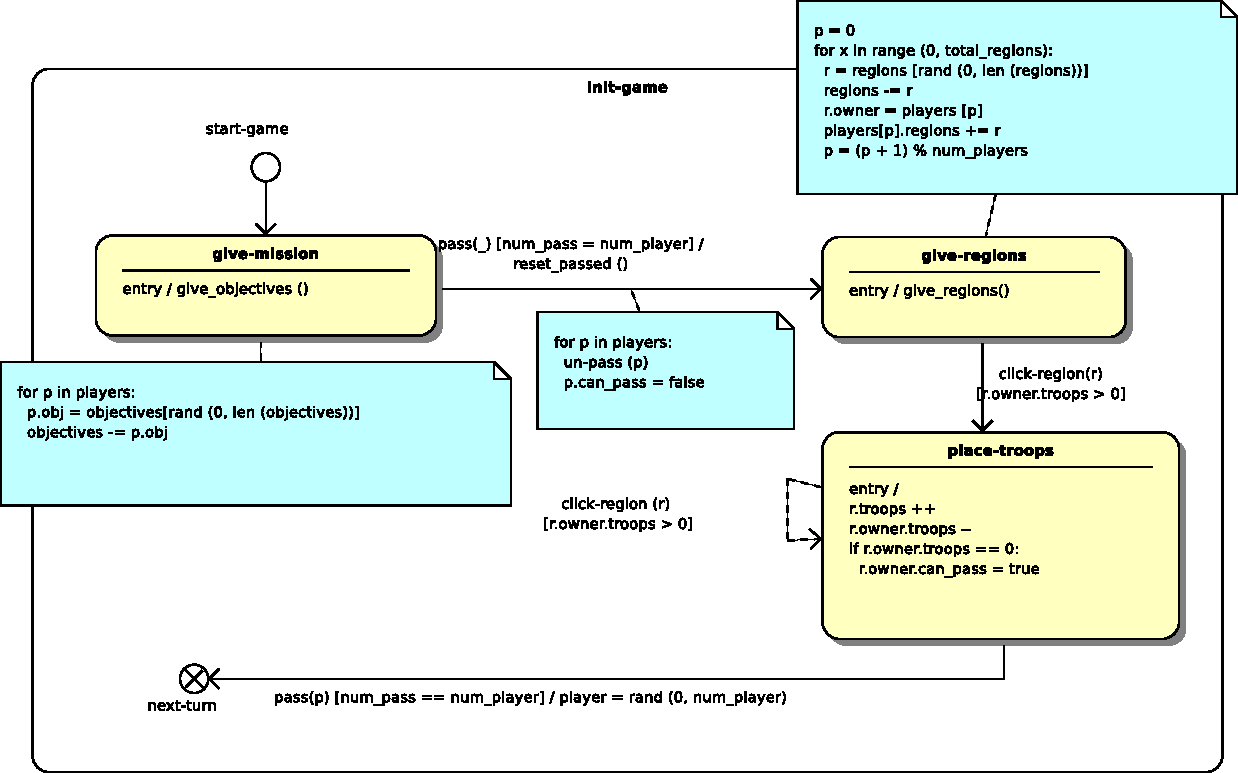
\includegraphics[width=15cm]{pic/3.pdf}
  \caption{\texttt{init-game} state machine.}
  \label{fig:sm:init-game}
\end{figure}

\subsection{\texttt{in-game-menu} state machine.}
\begin{figure}[H]
  \centering
  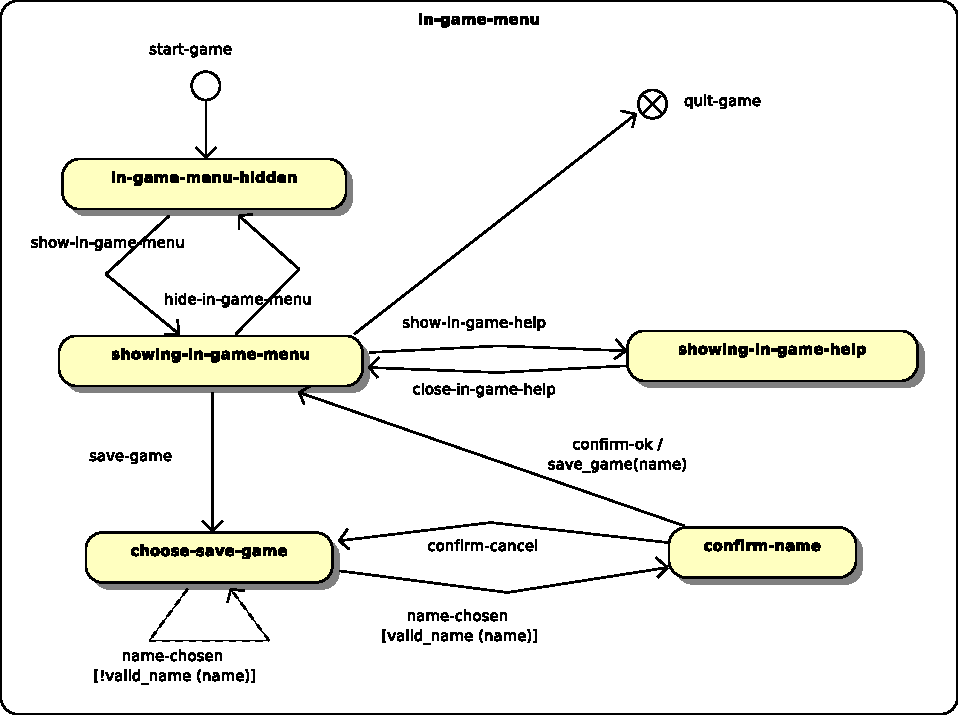
\includegraphics[width=14cm]{pic/4.pdf}
  \caption{\texttt{in-game-menu} state machine.}
  \label{fig:sm:in-game-menu}
\end{figure}

\subsection{\texttt{player-menu} state machine}
\begin{figure}[H]
  \centering
  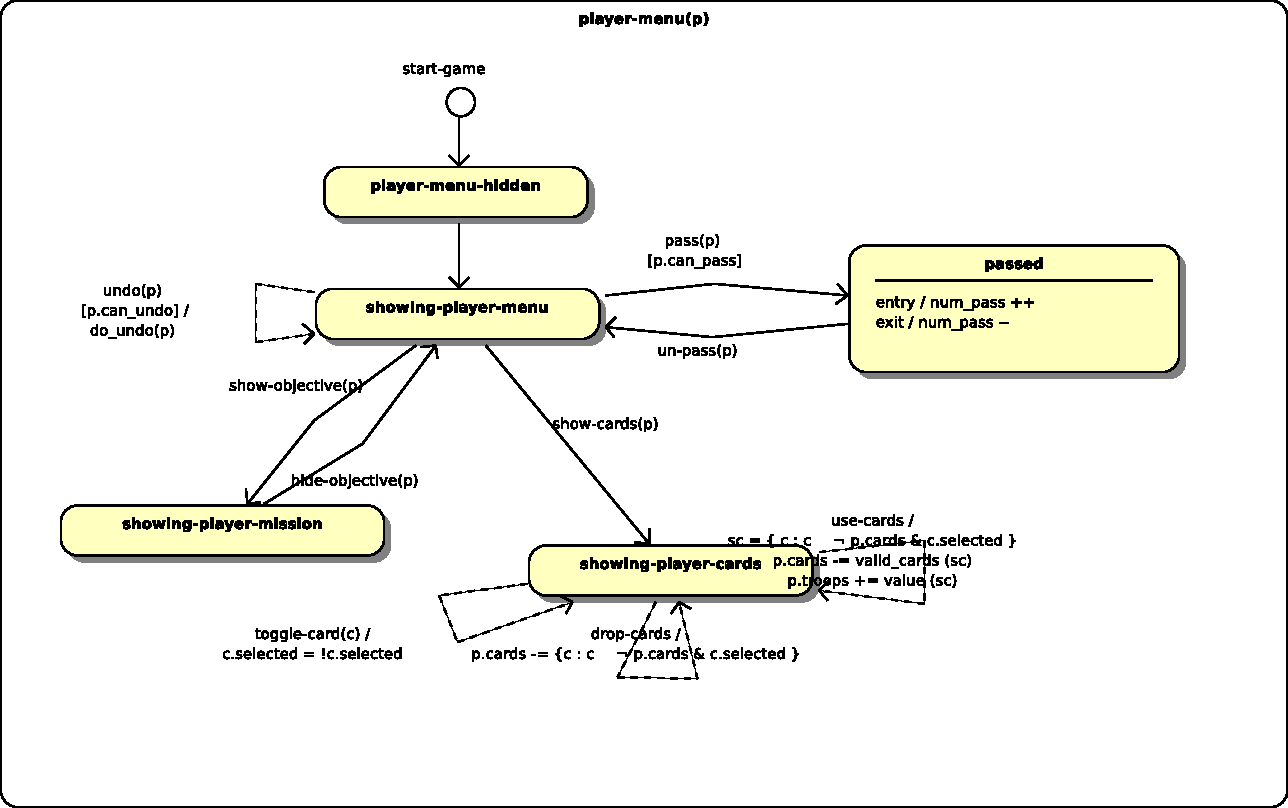
\includegraphics[width=15cm]{pic/5.pdf}
  \caption{Global state machine.}
  \label{fig:sm:player-menu}
\end{figure}

\subsection{\texttt{one-turn} state machine}
\begin{figure}[H]
  \centering
  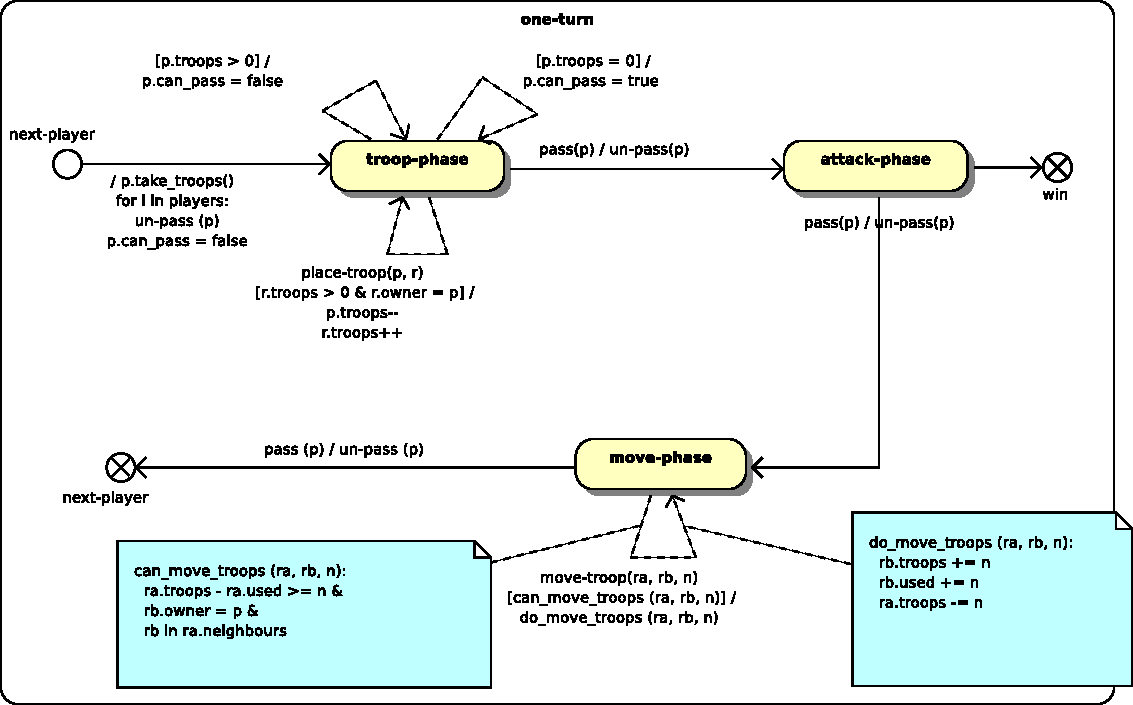
\includegraphics[width=15cm]{pic/6.pdf}
  \caption{\texttt{one-turn} state machine.}
  \label{fig:sm:one-turn}
\end{figure}

\subsection{\texttt{attack-phase} state machine}
\begin{figure}[H]
  \centering
  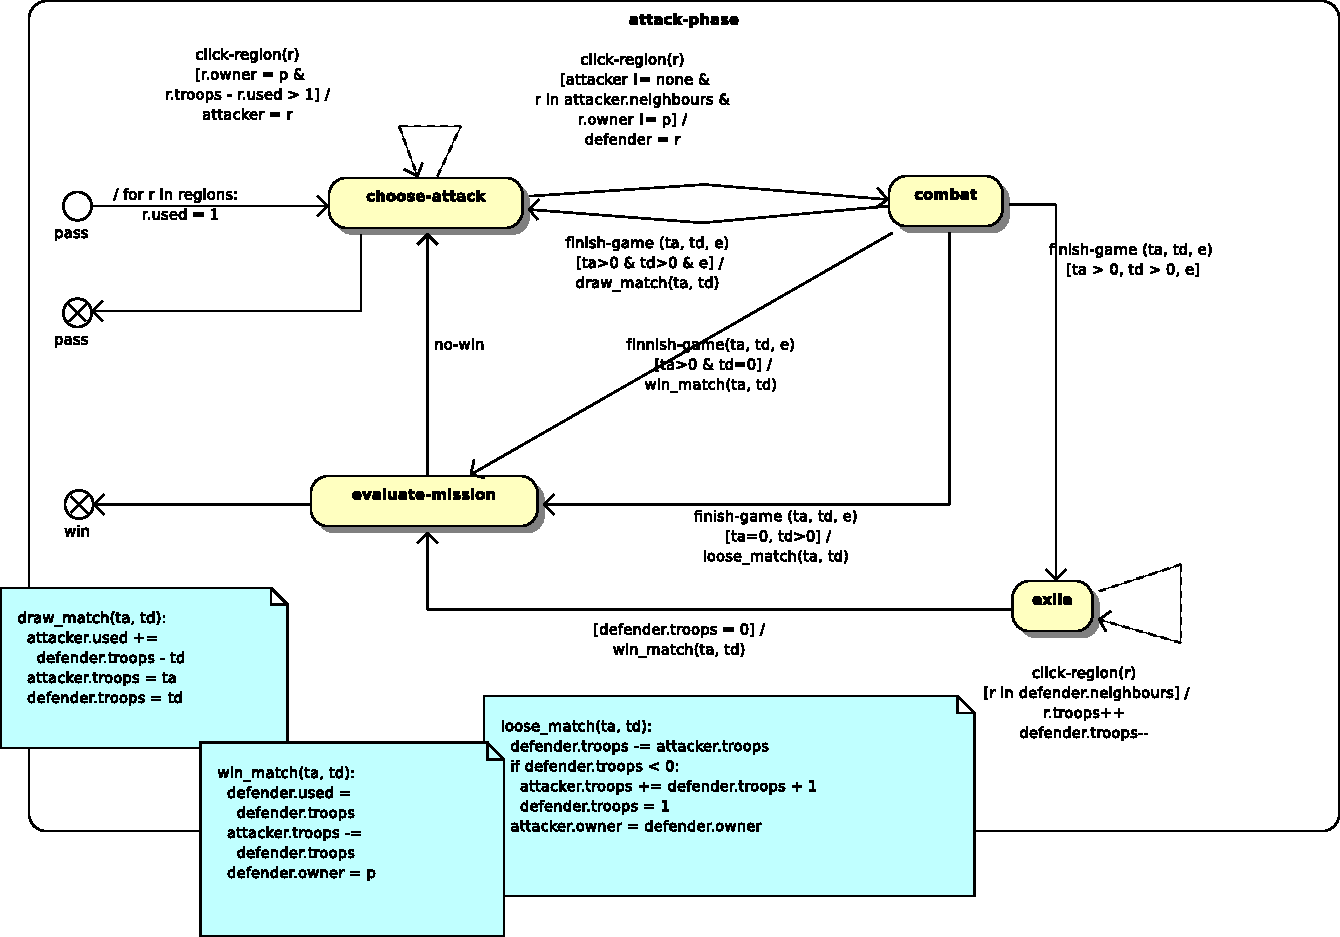
\includegraphics[width=15cm]{pic/7.pdf}
  \caption{\texttt{attack-phase} state machine.}
  \label{fig:sm:global}
\end{figure}


\section{Persistence}

\subsection{Introduction}
This section describes the different storage mechanism used by the
system, as the map (boards) where the game takes place, the status for
loading and loading games and the storage of player settings and profiles.

\subsection{Map}

In order to make the game more flexible and interesting, the players
will be able to create and use new maps for them games, than can be
larger or smaller (levering in this way the length of the game) or
have different and challenging topologies or resemble fantastic or
real places. The maps will be defined by a simple \texttt{XML}
(eXtensible Markup Language) file. The file is defined using
\texttt{DTD} (Document Type definition) to determine the grammar that
these must follow. The semantics of the different tags and attributes
that one may use in these files is encoded in comments in the
\texttt{DTD} file that is now shown.

\subsection{Map file definition \texttt{map-file.dtd}}

\lstinputlisting[language=XML]{../file-formats/map-file.dtd}

\subsection{Game saving and loading}

As this game matches can take very long, specially in big maps or in
presence of multiple players, it is very nice to have a feature to
store and load games.

To achieve this, the best system is to correctly separate the concerns
of \emph{state} and \emph{behaviour} in the model, the former being
intended to be stored persistently modelling an instantaneous image of
the game world and the later concentrating on local and dynamic
reactivity of the system. This allows us to easily use Python
\emph{object pickling} to automatically serialise the state and dump
it into a file. For more information about object pickling visit:

\url{http://docs.python.org/library/pickle.html}

It is still unsure weather a second file providing metadata about the
save game (possibly using XML) would actually be needed.

\begin{todo}[Juan Pedro]
  This last phrase probably should be changed into something concrete in
  the final version of the document.
\end{todo}

\subsection{Customisation}

The application uses a customisation system that relies on the
\texttt{ConfNode} class. This system provide a hierarchical
multi-backend and observable configuration system. By hierarchical we
mean that the configuration is composed of a tree of values, where a
node in the configuration can have some other child values. By
multi-backend we mean that the actual persistence of this
configuration is hidden to most of part of the application and can be
changed at runtime. This could allow to have a system that can either
store the configuration using \texttt{gconf}, the Windows registry,
\texttt{INI} files or \texttt{XML} files. Currently, a \texttt{XML}
backend is implemented that is limited to \texttt{str}, \texttt{int},
\texttt{bool} and \texttt{float} values. By observable we ultimately
mean that one can register slots (callbacks) into one node to be
notified on updates, turning the configuration system into a
\emph{model} (using the MVC terminology) that aids in separating the
concerns of the objects that modify the configuration.
\emph{controllers}, and the ones that whose behaviour depend on it,
\emph{views}.

The configuration nodes are named by a string, and the path to a node
can be encoded using the a dot \texttt{'.'} to relate a parent node to
its child. The following sections describe the configuration values
used by the application.

\begin{todo}[Juan Pedro]
  Should I make class diagrams of the \texttt{base} module that I
  imported from the other project so this paragraph is more clear? (It
  currently refers to classes, i.e. the ConfNode, that are not
  modelled anywhere!)
\end{todo}

\subsubsection{SFML configuration}

These values are able to configure how the game shows on the
screen. Probably most of them will be useless in the final release as
the video-game console will use fixed parameters, but they are useful
for debugging and can aid in a later PC port.

\begin{table}[h]
  \centering
  \begin{tabular}[h]{l|c|p{7cm}}
    Option & Type & Meaning \\ \hline\hline
    
    \texttt{jagsat.sfml.width} & \texttt{int} & Screen width in
    pixels.\\
    \texttt{jagsat.sfml.height} & \texttt{int} & Screen height in
    pixels.\\
    \texttt{jagsat.sfml.bpp} & \texttt{int} & Colour depth in bits per pixel.\\
    \texttt{jagsat.sfml.vsynch} & \texttt{bool} & Vertical
    synchronization activated. \\
    \texttt{jagsat.sfml.fps} & \texttt{int} & Execution frames per
    second. \\
    \texttt{jagsat.sfml.full} & \texttt{bool} & Use full-screen
    or windowed mode.    
  \end{tabular}
\end{table}


\subsubsection{Player profiles}

It is very useful to store game profiles. For example, a user Mike might
usually play with his friends Tom and Anna some days, and other days
with his father John and his mother Lisa. To avoid setting up the
player position, colors, and the map that he likes to play in these
contexts, he could use a \emph{profile} called \emph{Family} or
\emph{Friends} for either case.

To support this functionality with minimum code boilerplate our
hierarchical customisation system can store this profiles in a node
for each.

\begin{table}[h]
  \centering
  \begin{tabular}[h]{l|c|p{5.5cm}}
    Option & Type & Meaning \\ \hline\hline
    
    \texttt{jagsat.profiles.\emph{profile}} & \texttt{None} & A
    node containing all the options of a given profile \emph{profile}.
  \end{tabular}
\end{table}

Each profile contains all the options needed to set up a game. We will
now shorten \texttt{jagsat.profiles.\emph{profile}} as just
\texttt{\emph{profile}}.

\begin{table}[h]
  \centering
  \begin{tabular}[h]{l|c|p{7cm}}
    Option & Type & Meaning \\ \hline\hline
    
    \texttt{\emph{profile}.player\_1} & \texttt{None} & Options of the
    first player. \\
    \texttt{\emph{profile}.player\_2} & \texttt{None} & Options of the
    second player. \\
    \texttt{...} & \texttt{...} & ... \\
    \texttt{\emph{profile}.player\_6} & \texttt{None} & Options of the
    sixth player. \\
    \texttt{\emph{profile}.map} & \texttt{str} & File name of the map. \\
  \end{tabular}
\end{table}

For each player, we have the following set of options.

\begin{table}[h]
  \centering
  \begin{tabular}[h]{l|c|p{7cm}}
    Option & Type & Meaning \\ \hline\hline
    
    \texttt{player\_\emph{n}.name} & \texttt{str} & Name of the
    player. \\
    \texttt{player\_\emph{n}.color} & \texttt{int} & Colour of the player. \\
    \texttt{player\_\emph{n}.position} & \texttt{int} & Position of
    the player around the table, where $position \in [1, 6]$. \\
  \end{tabular}
\end{table}

\section{User interface}

This section includes a series of mock-ups of the user interface. The
different elements are tagged with letters and a table shows the
behaviour associated with each element.

In some way, these mock-ups clearly reflect what is happening on the
state machines, so it could ease the reader to go back and forward
from/to the state machines while reading this section of the document
to get a deeper understanding of the system.

\newpage
\subsection{Main menu}\label{mock:71}

\subsubsection{Configuration}\label{mock:711}

\begin{figure}[H]
  \centering
  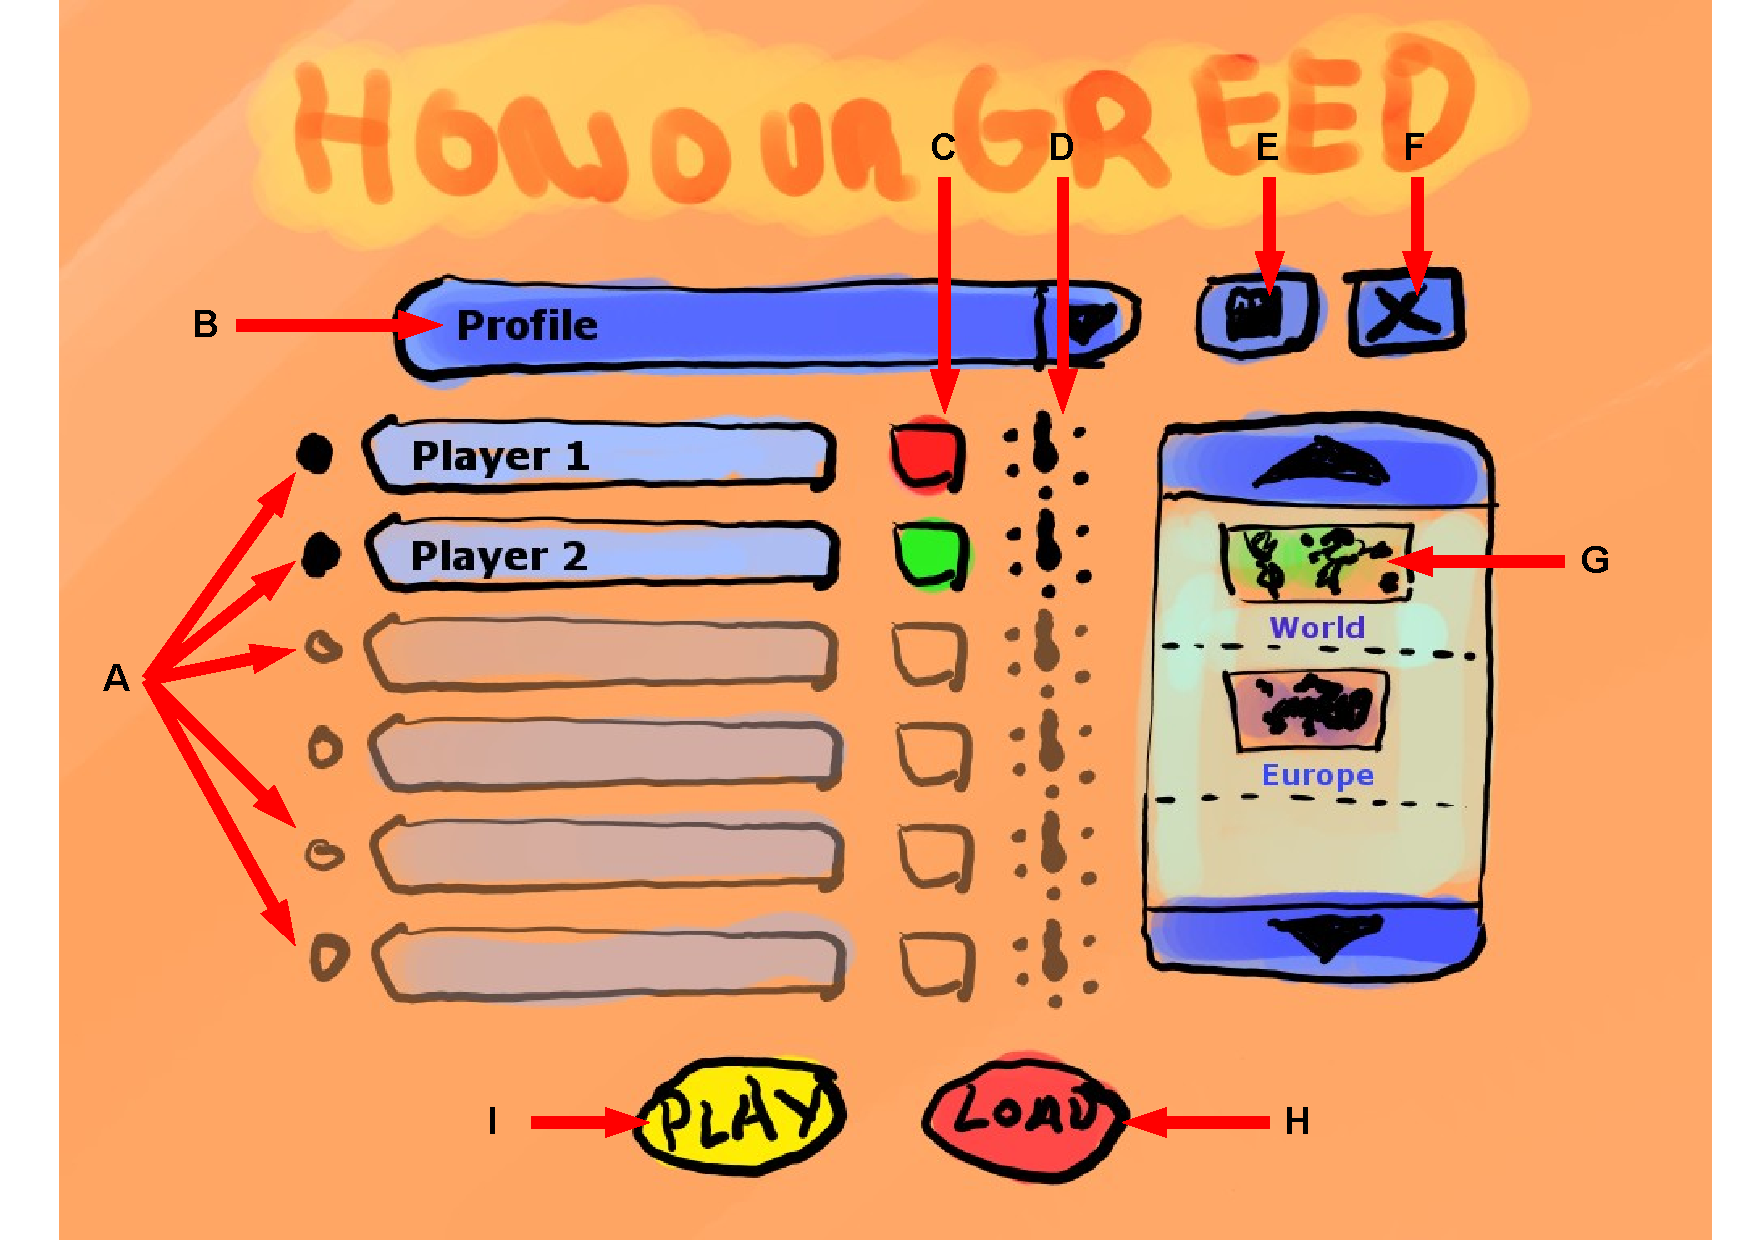
\includegraphics[width=11cm]{pic/mocks/1-1.pdf}
\end{figure}

\begin{table}[H]
\small
\centering
\begin{tabular}{c|p{5cm}|p{7cm}}
& Name & Action \\ \hline\hline
%%%
A
&Players configuration
&By clicking the black left button the player will be activated. By clicking the player name button the keyboard will appear to change player name.
\\B
&Profile menu
&Displays profile menu with profiles list
\\C
&Player colour configuration
&By clicking the button player color changes
\\D
&Player position configuration
&Points the player position around the device
\\E
&Save profile
&Shows \ref{mock:712} menu
\\F
&Delete profile
&Deletes profile
\\G
&Possible maps
&Map selected will be remarked.
\\H
&Load game
&Shows \ref{mock:713} menu
\\I
&Play game
&Starts game if the actual config is valid.
\end{tabular}
\end{table}

\subsubsection{Save profile}\label{mock:712}

\begin{figure}[H]
  \centering
  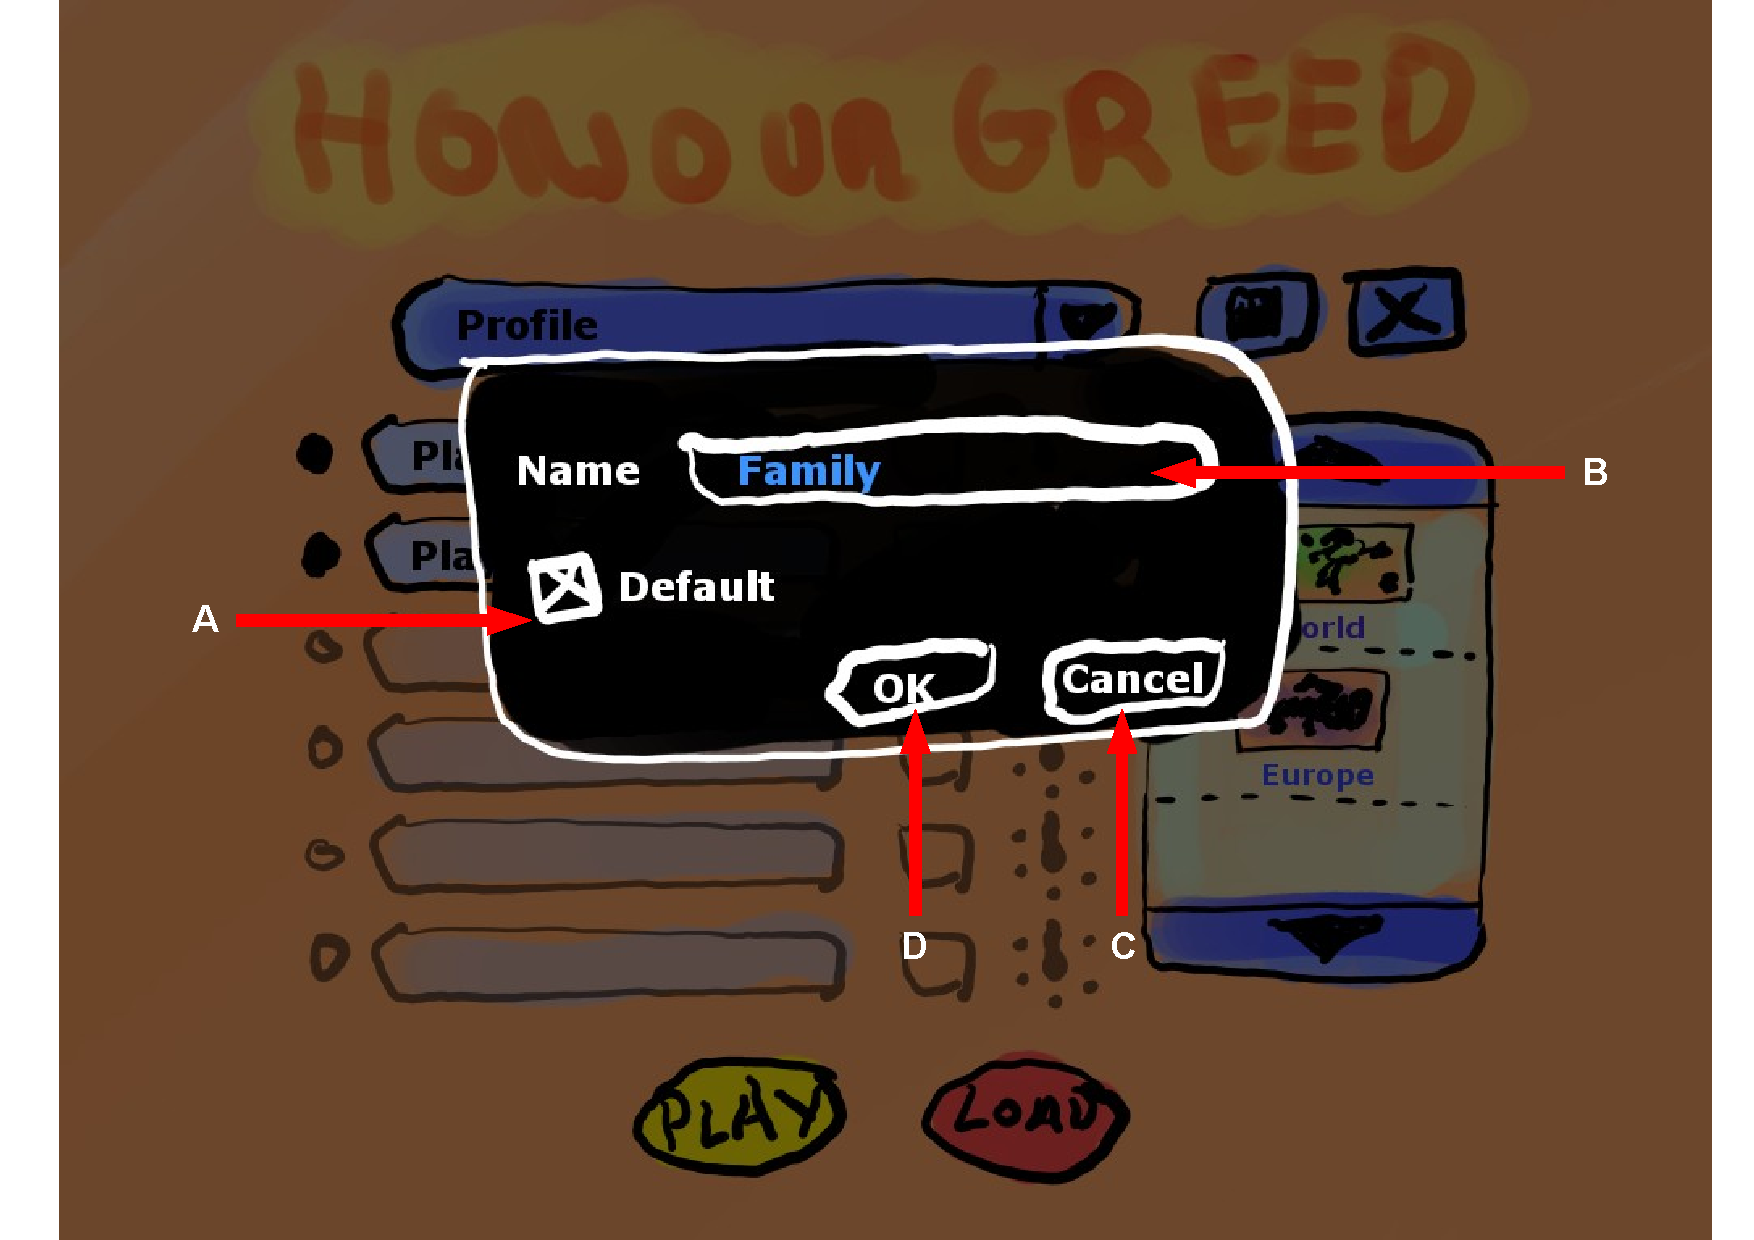
\includegraphics[width=11cm]{pic/mocks/1-2.pdf}
\end{figure}

\begin{table}[H]
\small
\centering
\begin{tabular}{c|p{5cm}|p{7cm}}
& Name & Action \\ \hline\hline
%%%
A
&Set profile as default
&This profile will be shown as marked in \ref{mock:711}B
\\B
&Profile name.
&
\\C
&Cancel button:
&Back to \ref{mock:711} without changes
\\D
&Ok button
&Back to \ref{mock:711} with profile changes
\end{tabular}
\end{table}

\subsubsection{Load game}\label{mock:713}

\begin{figure}[H]
  \centering
  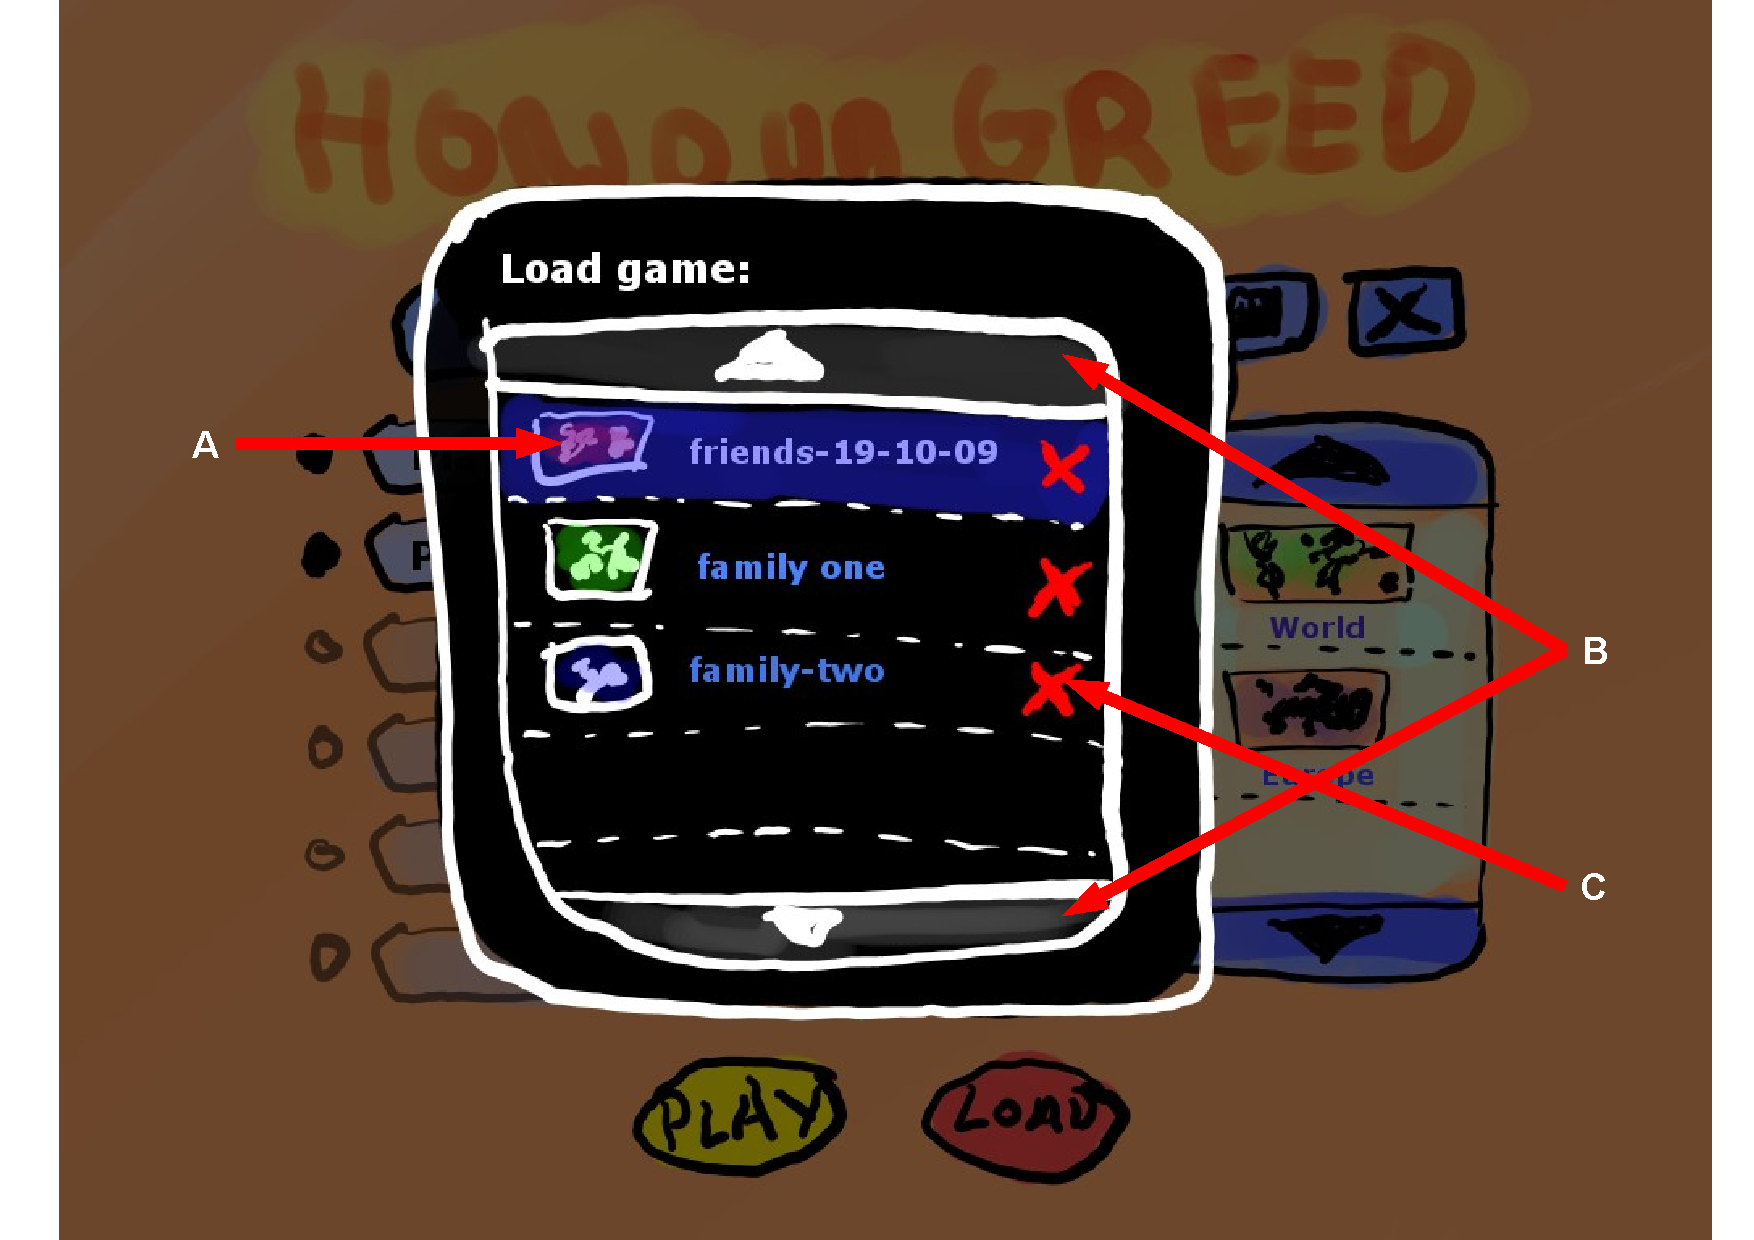
\includegraphics[width=11cm]{pic/mocks/1-3.pdf}
\end{figure}

\begin{table}[H]
\small
\centering
\begin{tabular}{c|p{5cm}|p{7cm}}
& Name & Action \\ \hline\hline
%%%
A
&Map preview
&Little picture of the kind of map played in this game.
\\B
&Up/Down buttons
\\C
&Delete saved game.

\end{tabular}
\end{table}

\subsubsection{Confirmation}\label{mock:714}
\begin{figure}[H]
  \centering
  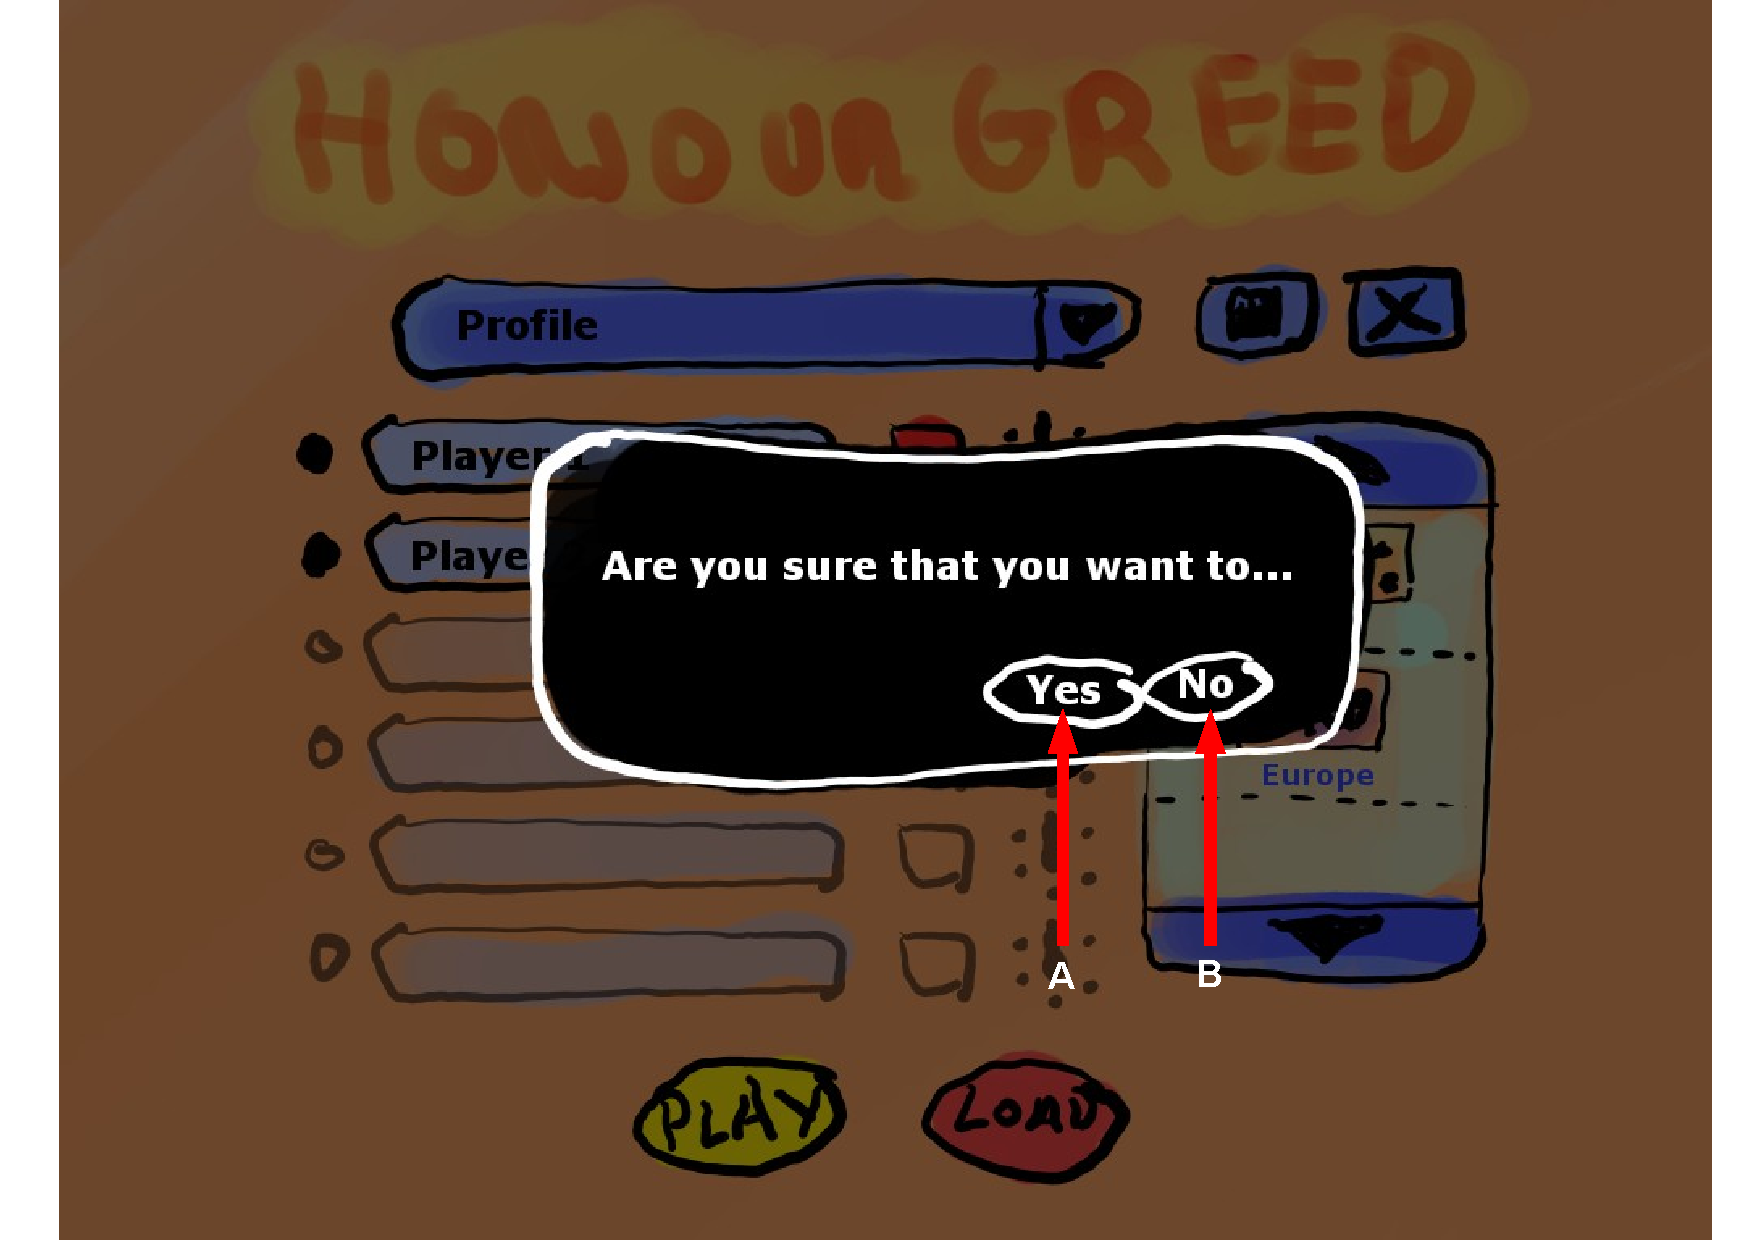
\includegraphics[width=11cm]{pic/mocks/1-4.pdf}
\end{figure}

\begin{table}[H]
\small
\centering
\begin{tabular}{c|p{5cm}|p{7cm}}
& Name & Action \\ \hline\hline
%%%
A
&Confirm
\\B
&Cancel
\end{tabular}
\end{table}

\subsection{In game player menu}\label{mock:72}

\subsubsection{Overview}\label{mock:721}

\begin{figure}[H]
  \centering
  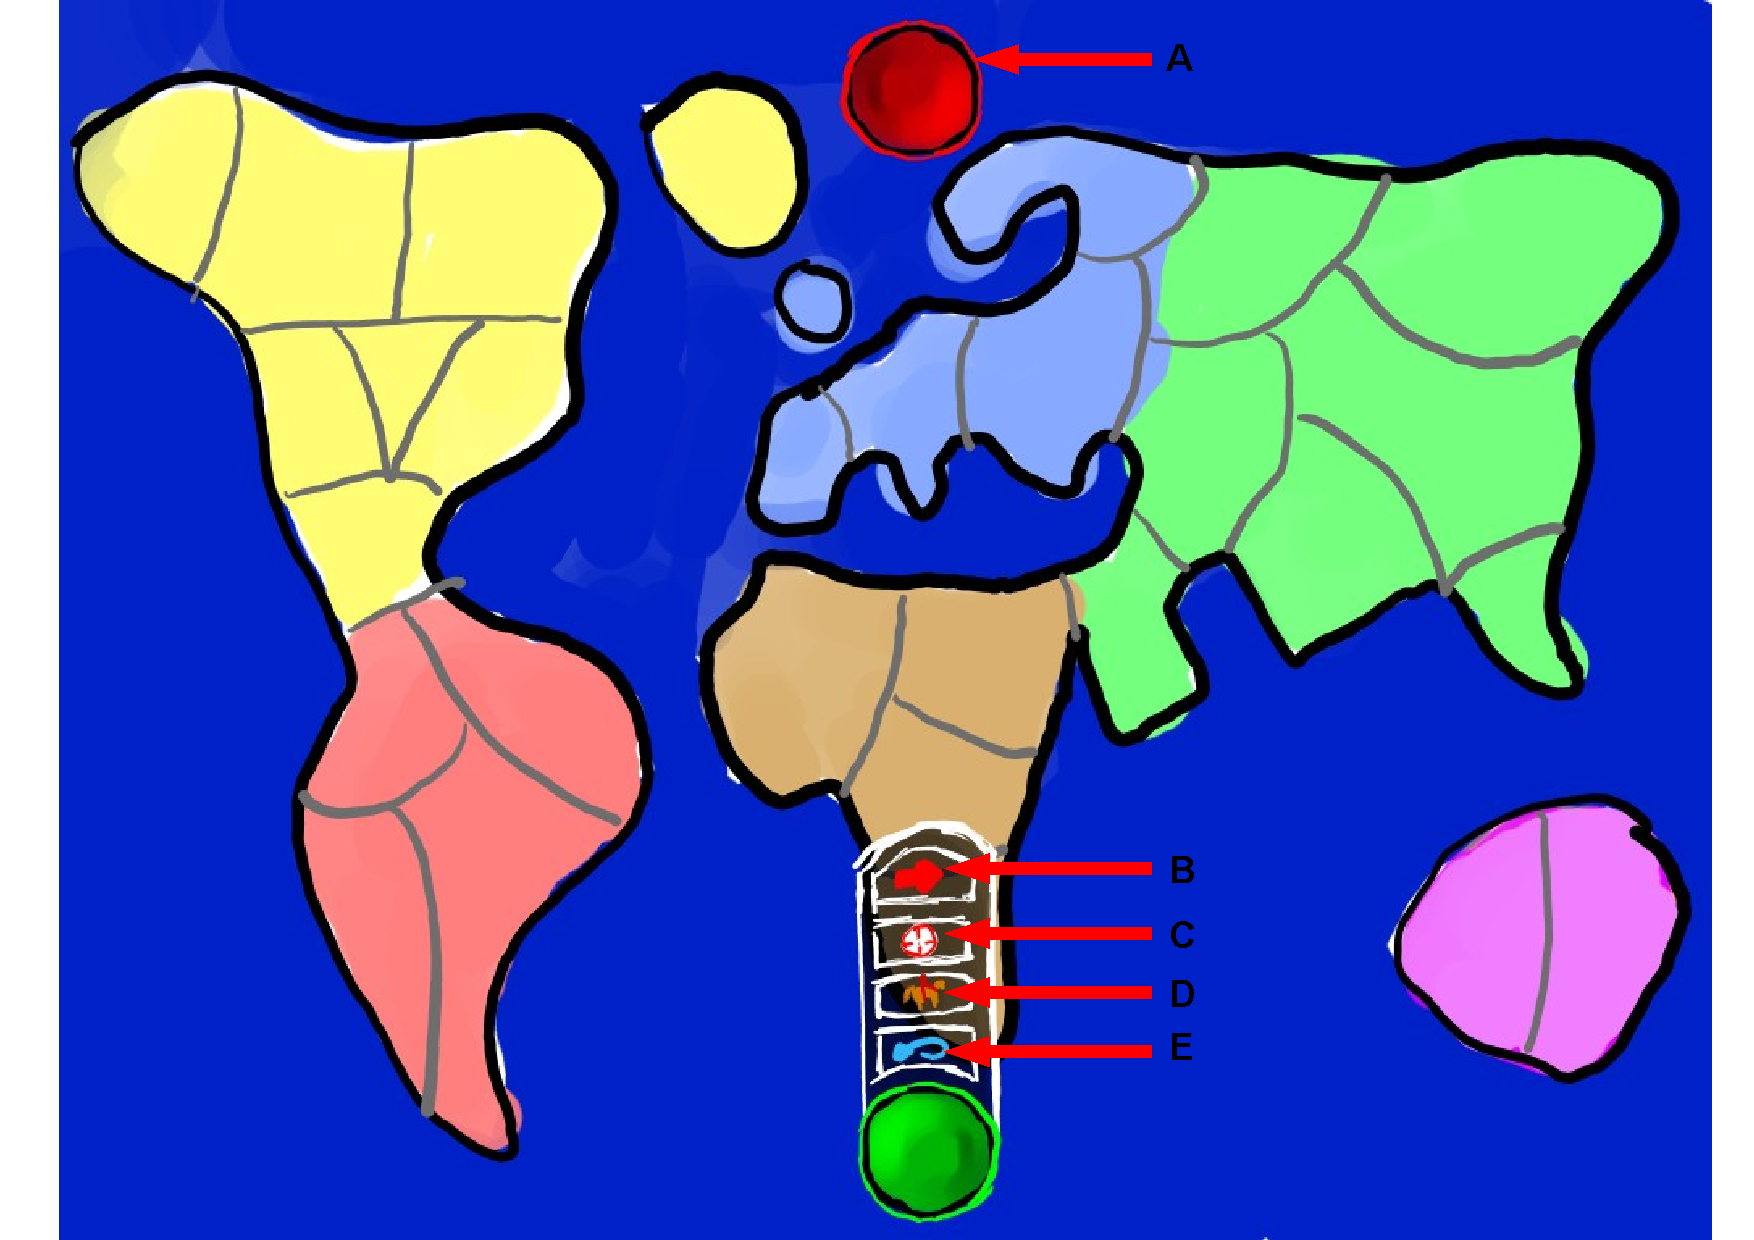
\includegraphics[width=11cm]{pic/mocks/2-1.pdf}
\end{figure}

\begin{table}[H]
\small
\centering
\begin{tabular}{c|p{5cm}|p{7cm}}
& Name & Action \\ \hline\hline
%%%
A
&Player menu button
&Shows the menu with options [B,E]
\\B
&''Next'' button
&Perform the action “next” if avail[able
\\C
&''Objective'' button
&Shows objective \ref{mock:722}
\\D
&''Cards'' button
&Shows cards \ref{mock:723}
\\E
&''Undo'' button
&Undo the previous action.
\end{tabular}
\end{table}


\subsubsection{Objective}\label{mock:722}

\begin{figure}[H]
  \centering
  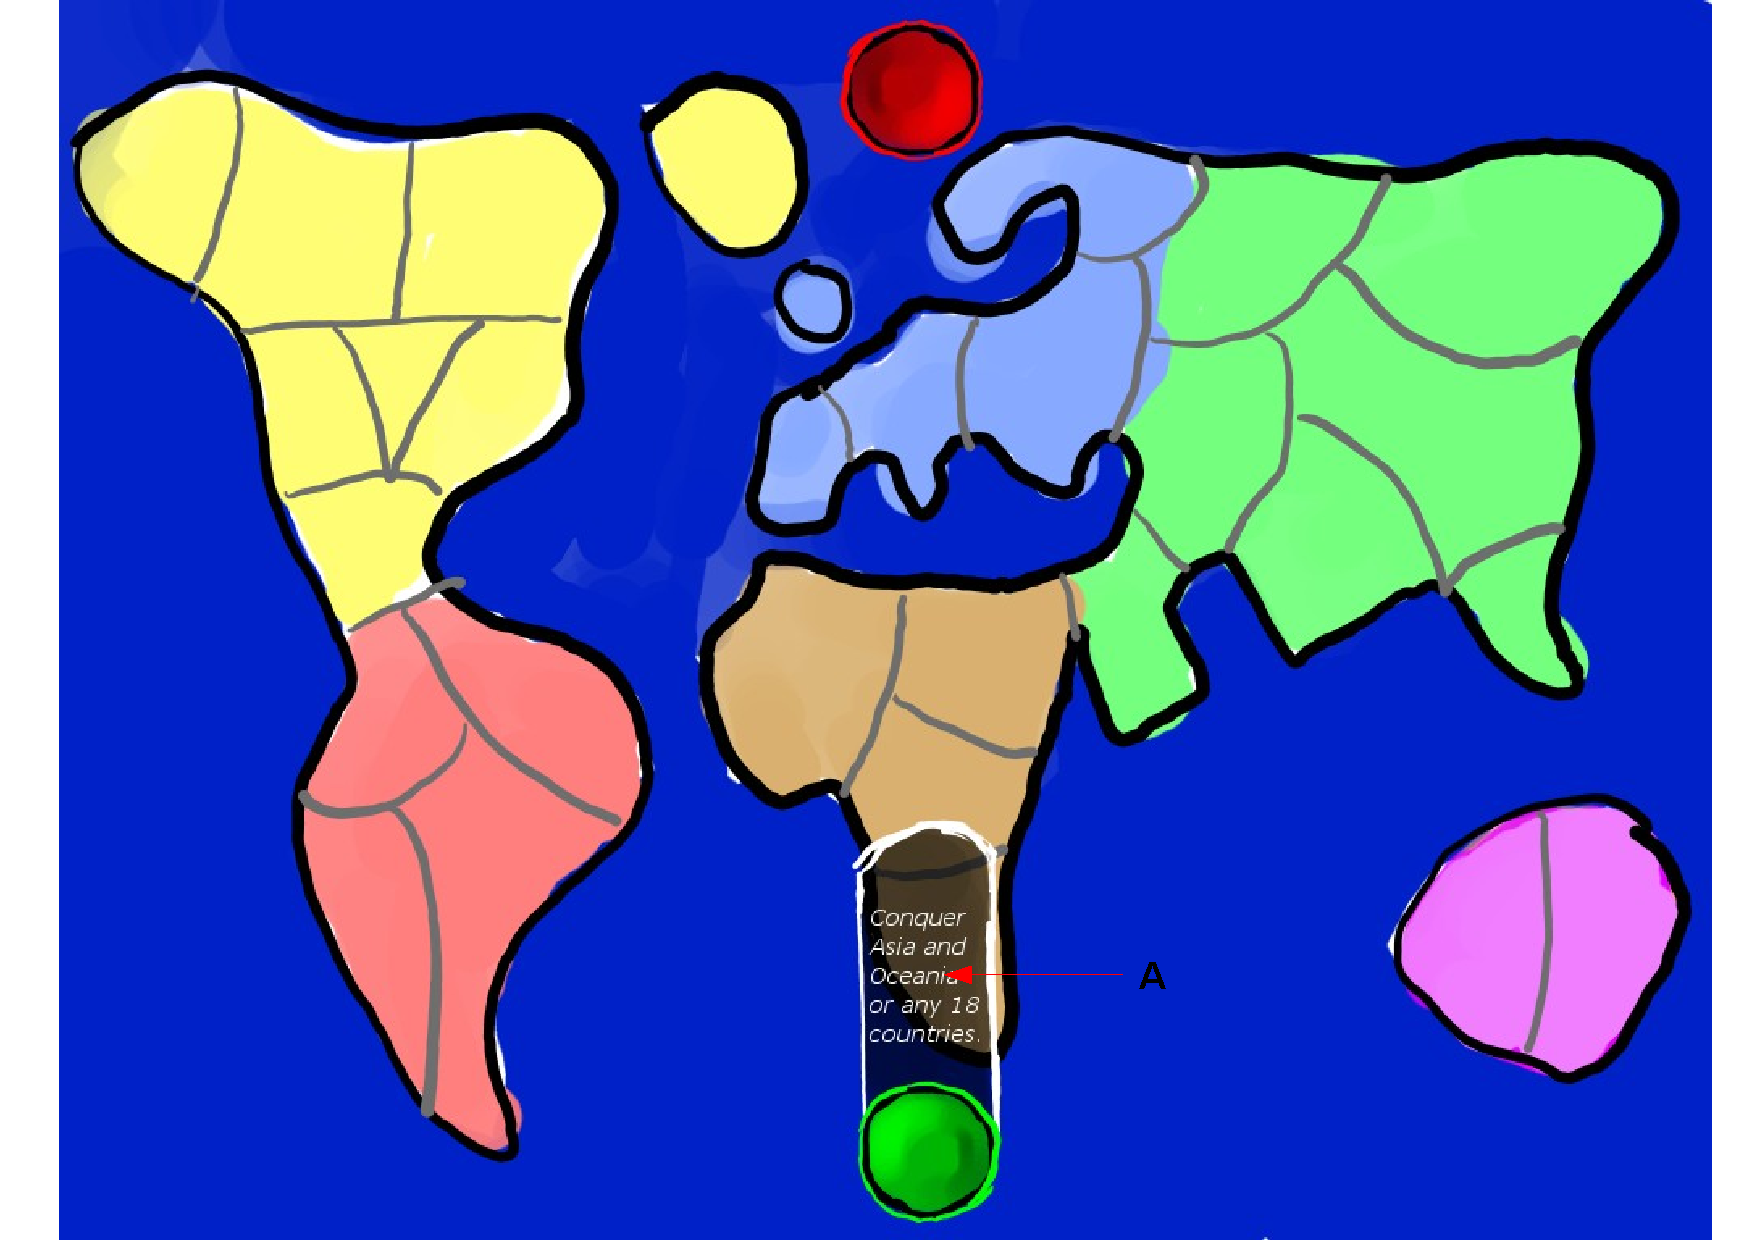
\includegraphics[width=11cm]{pic/mocks/2-2.pdf}
\end{figure}

\begin{table}[H]
\small
\centering
\begin{tabular}{c|p{5cm}|p{7cm}}
& Name & Action \\ \hline\hline
%%%
A
&Objective text
&Hides the objective text
\end{tabular}
\end{table}

\newpage
\subsubsection{Cards}\label{mock:723}

\begin{figure}[H]
  \centering
  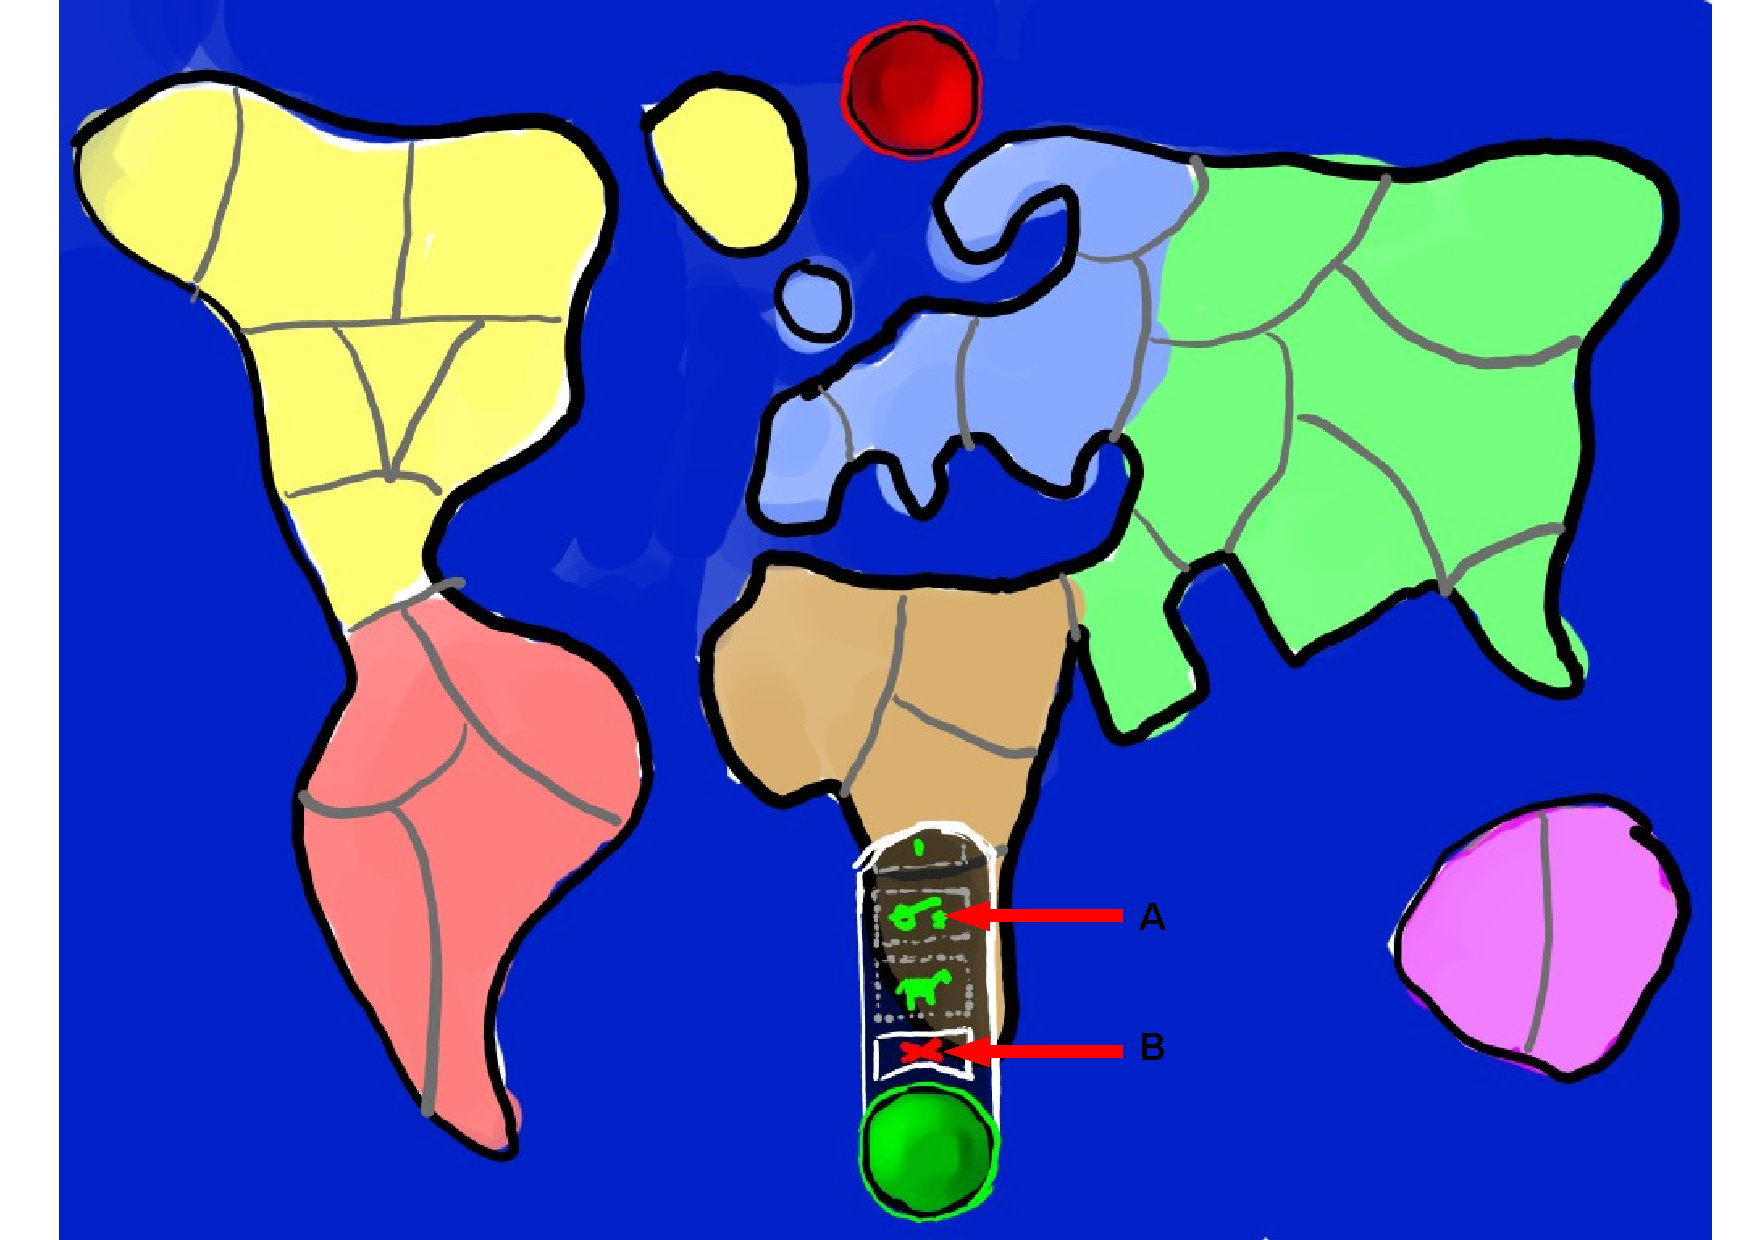
\includegraphics[width=11cm]{pic/mocks/2-3.pdf}
\end{figure}

\begin{table}[H]
\small
\centering
\begin{tabular}{c|p{5cm}|p{7cm}}
& Name & Action \\ \hline\hline
%%%
A
&Cards
&Select the cards that the player owns.
\\B
&''Exit'' button
&Back to \ref{mock:721}
\end{tabular}
\end{table}

\newpage
\subsubsection{Cards selection}\label{mock:724}

\begin{figure}[H]
  \centering
  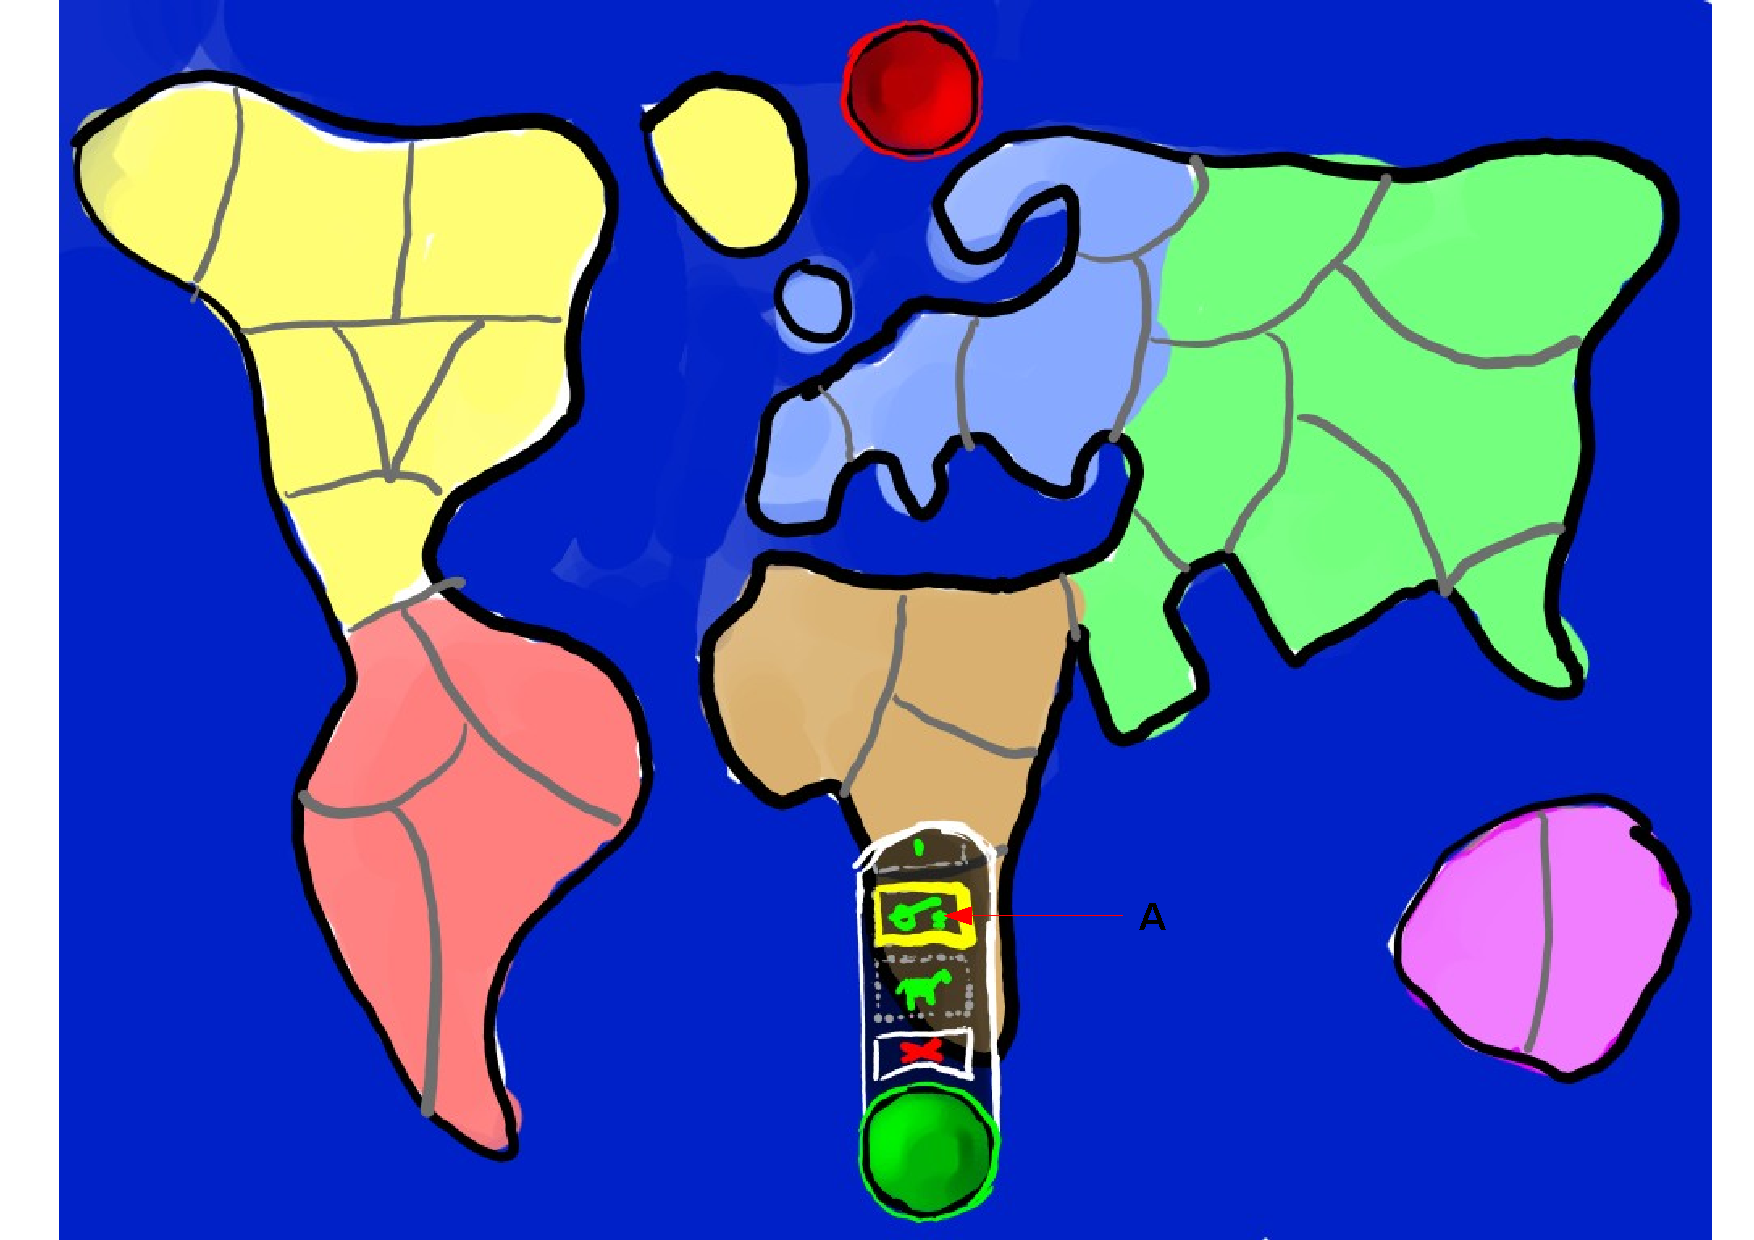
\includegraphics[width=11cm]{pic/mocks/2-4.pdf}
\end{figure}

\begin{table}[H]
\small
\centering
\begin{tabular}{c|p{5cm}|p{7cm}}
& Name & Action \\ \hline\hline
%%%
A
&Card
&Unselected card.
\end{tabular}
\end{table}


\subsection{Init phase}\label{mock:73}

\subsubsection{Objectives deal}\label{mock:731}

\begin{figure}[H]
  \centering
  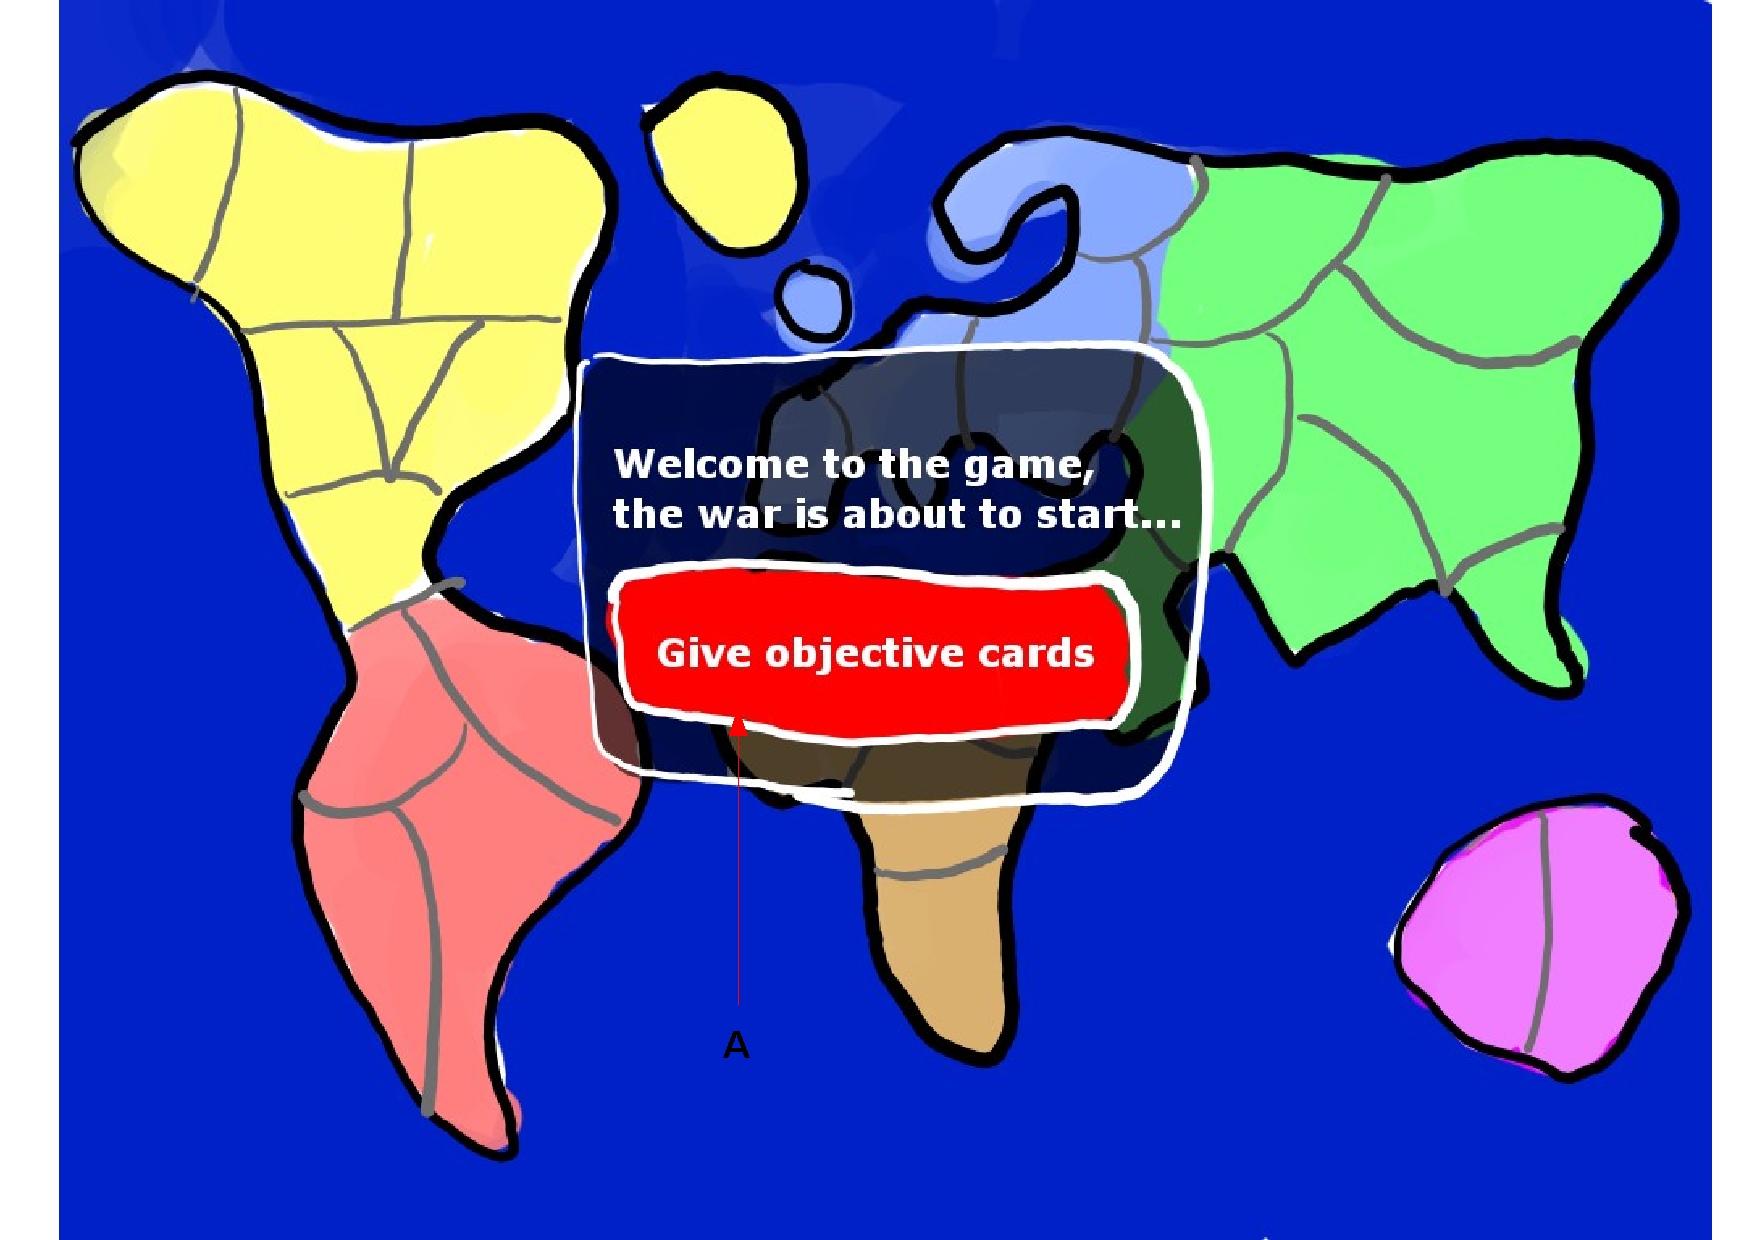
\includegraphics[width=11cm]{pic/mocks/3-1.pdf}
\end{figure}

\begin{table}[H]
\small
\centering
\begin{tabular}{c|p{5cm}|p{7cm}}
& Name & Action \\ \hline\hline
%%%
A
&Give objective
&Deals an objective to each player.
\end{tabular}
\end{table}


\subsubsection{Player positions}\label{mock:732}

\begin{figure}[H]
  \centering
  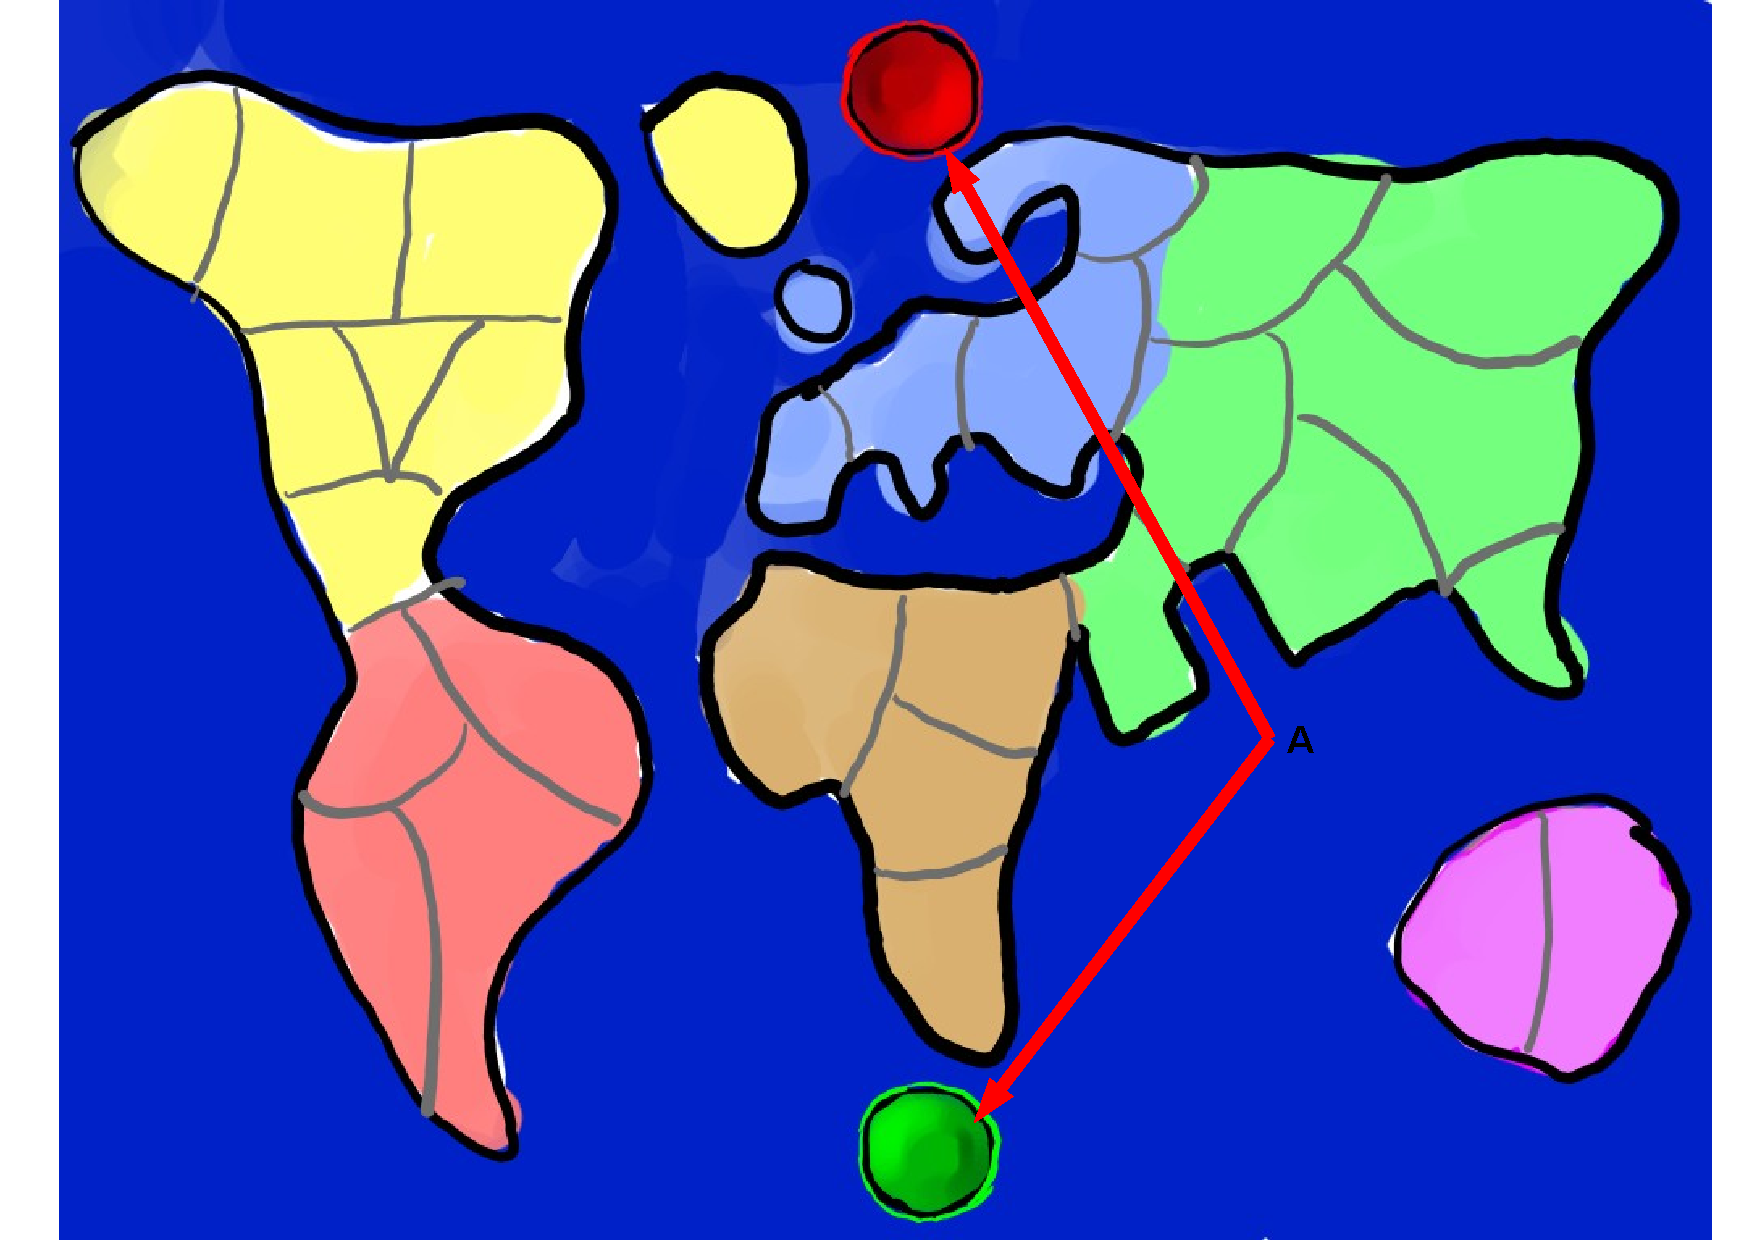
\includegraphics[width=11cm]{pic/mocks/3-2.pdf}
\end{figure}

\begin{table}[H]
\small
\centering
\begin{tabular}{c|p{5cm}|p{7cm}}
& Name & Action \\ \hline\hline
%%%
A
&Player menu
&Display player menu \ref{mock:72}
\end{tabular}
\end{table}

\newpage
\subsubsection{View objective active}\label{mock:733}

\begin{figure}[H]
  \centering
  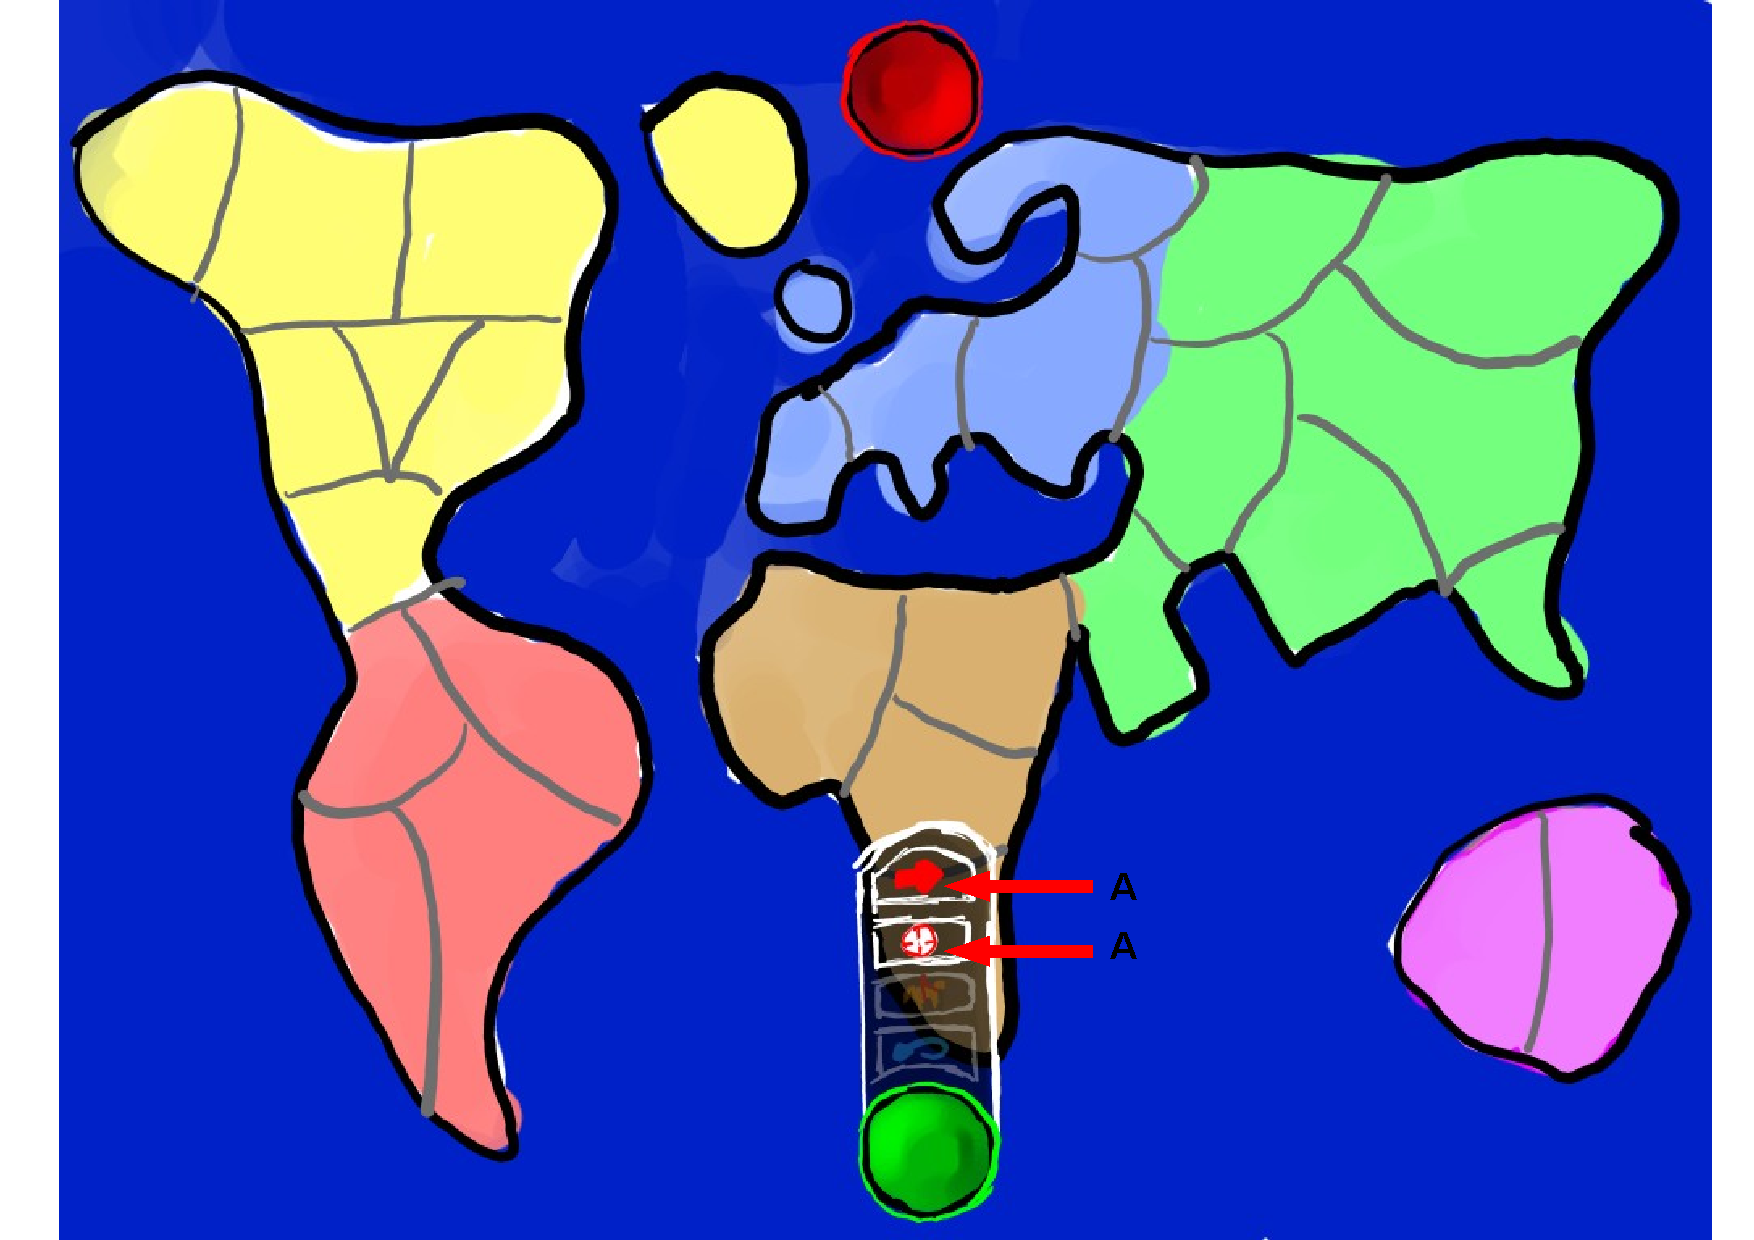
\includegraphics[width=11cm]{pic/mocks/3-3.pdf}
\end{figure}

\begin{table}[H]
\small
\centering
\begin{tabular}{c|p{5cm}|p{7cm}}
& Name & Action \\ \hline\hline
%%%
A
&Next
&Goes to \ref{mock:734}
\\B
&Show objective
&Goes to \ref{mock:722}
\end{tabular}
\end{table}

\subsubsection{Next button active}\label{mock:734}

\begin{figure}[H]
  \centering
  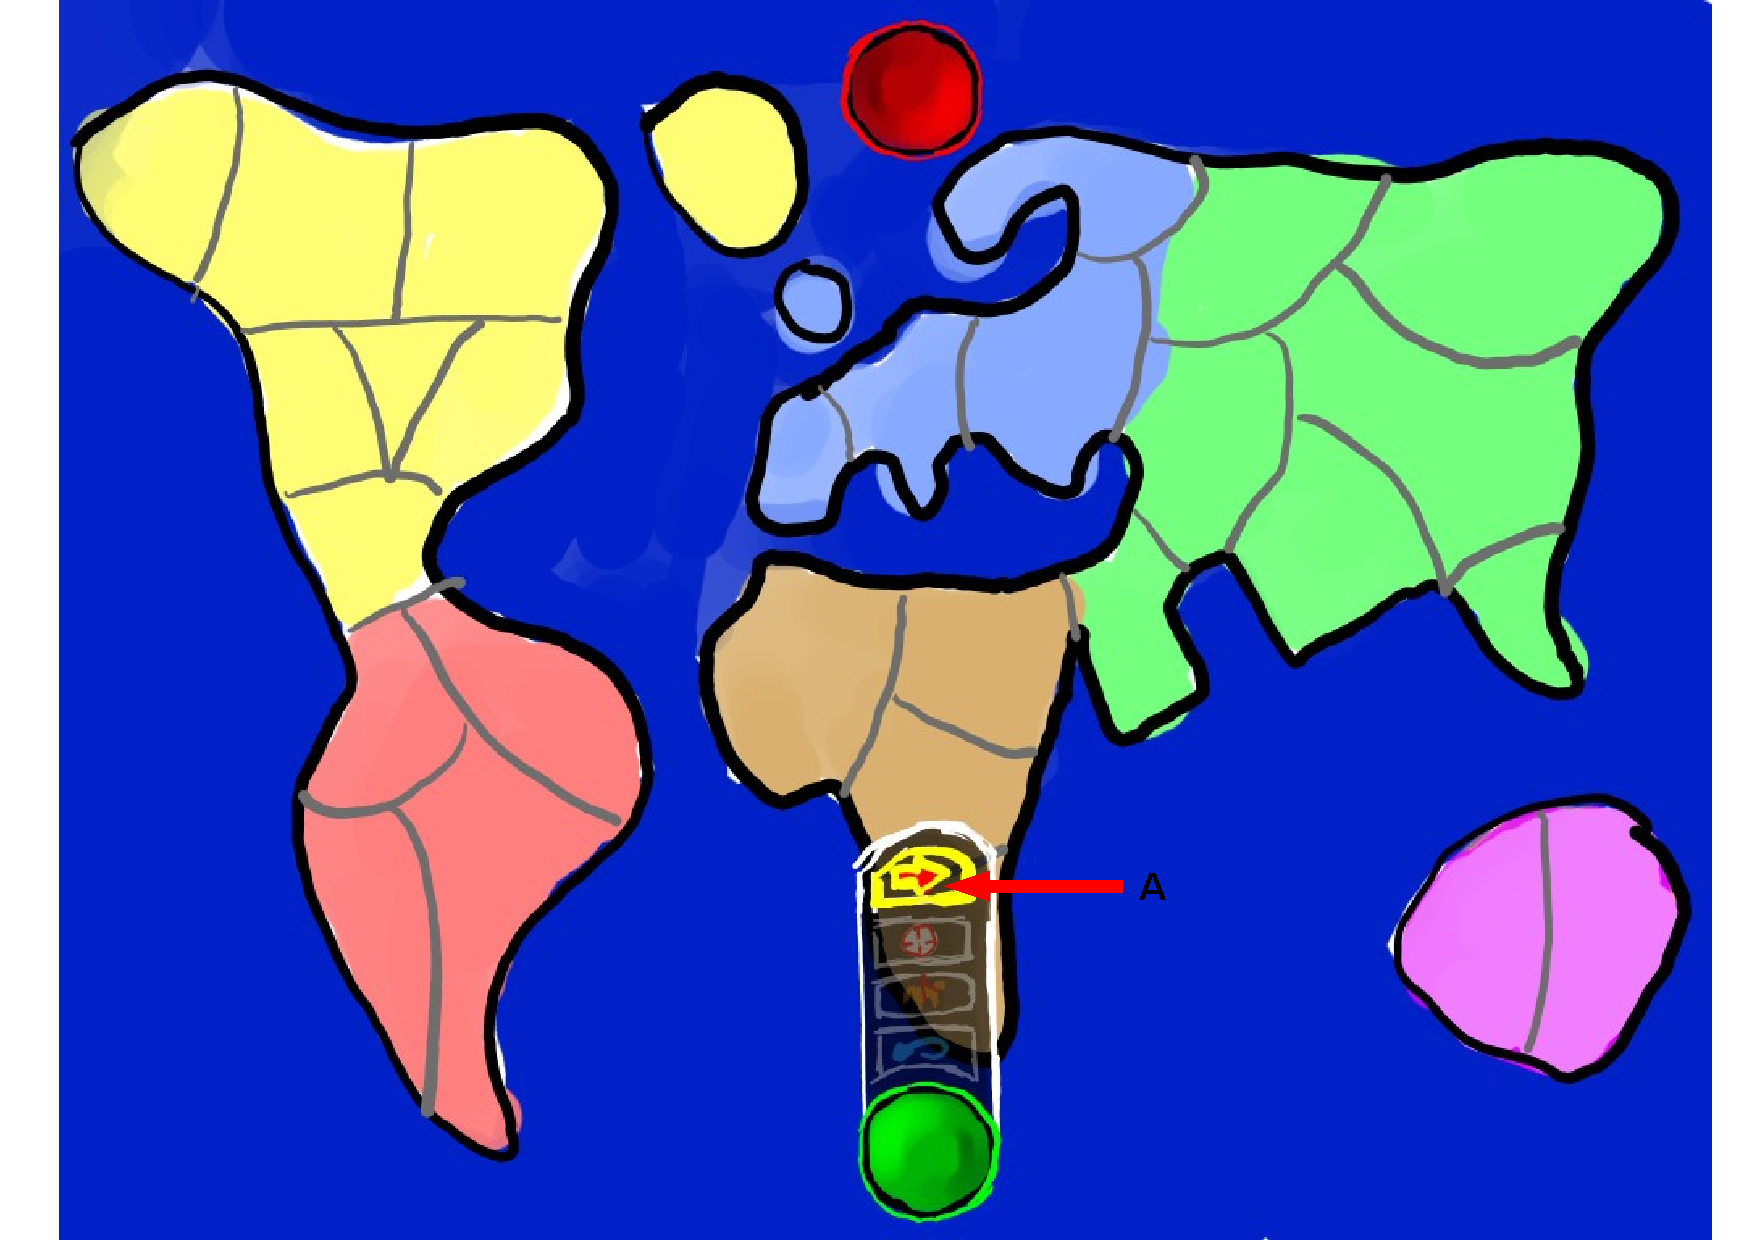
\includegraphics[width=11cm]{pic/mocks/3-4.pdf}
\end{figure}

\begin{table}[H]
\small
\centering
\begin{tabular}{c|p{5cm}|p{7cm}}
& Name & Action \\ \hline\hline
%%%
A
&Next button selected
&Goes to \ref{mock:735}
\end{tabular}
\end{table}


\newpage
\subsubsection{Troops placement}\label{mock:735}

\begin{figure}[H]
  \centering
  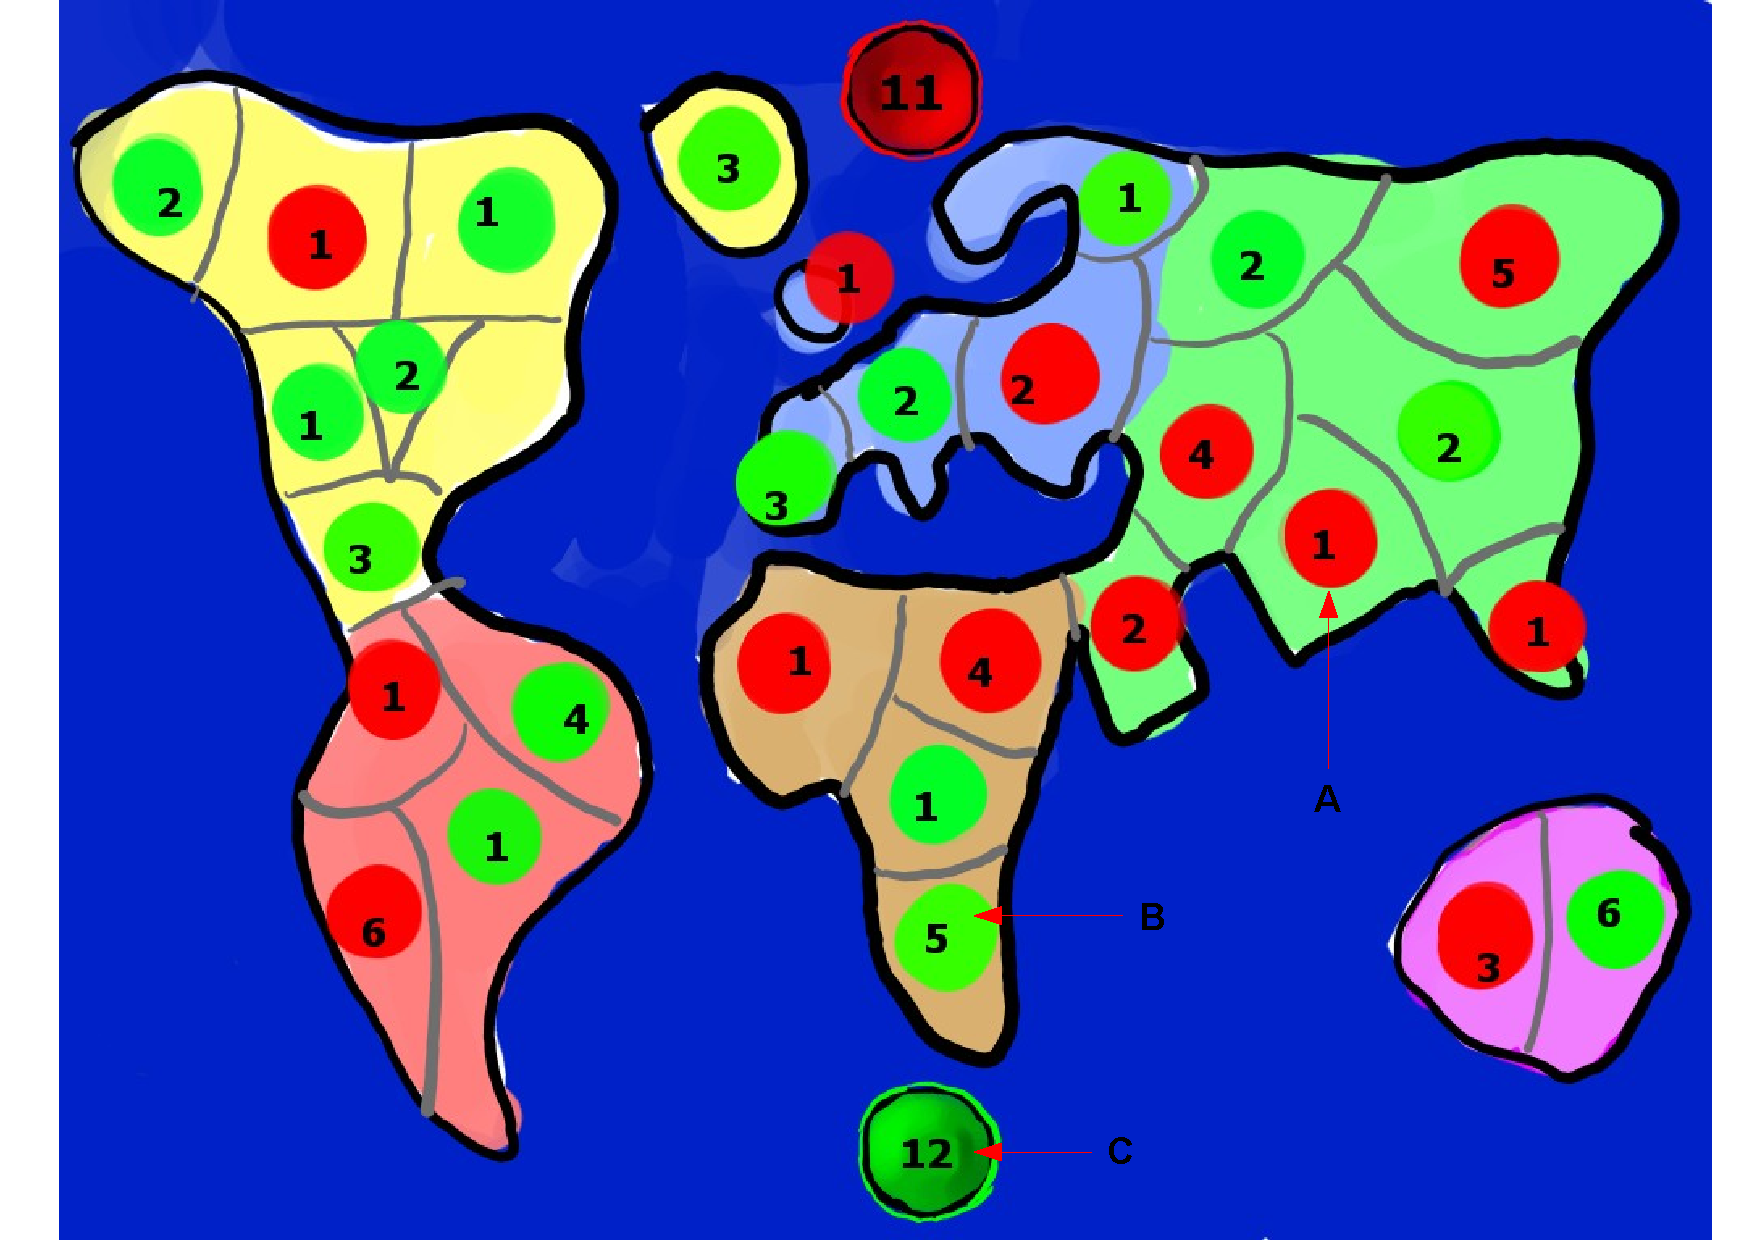
\includegraphics[width=11cm]{pic/mocks/3-5.pdf}
\end{figure}

\begin{table}[H]
\small
\centering
\begin{tabular}{c|p{5cm}|p{7cm}}
& Name & Action \\ \hline\hline
%%%
A
&Red region troops
&Increases number of red troops.
\\B
&Green region troops
&Increases number of green troops
\\C
&Troops left
&
\end{tabular}
\end{table}

\newpage
\subsubsection{Finish troop placement - Next button active}\label{mock:736}

\begin{figure}[H]
  \centering
  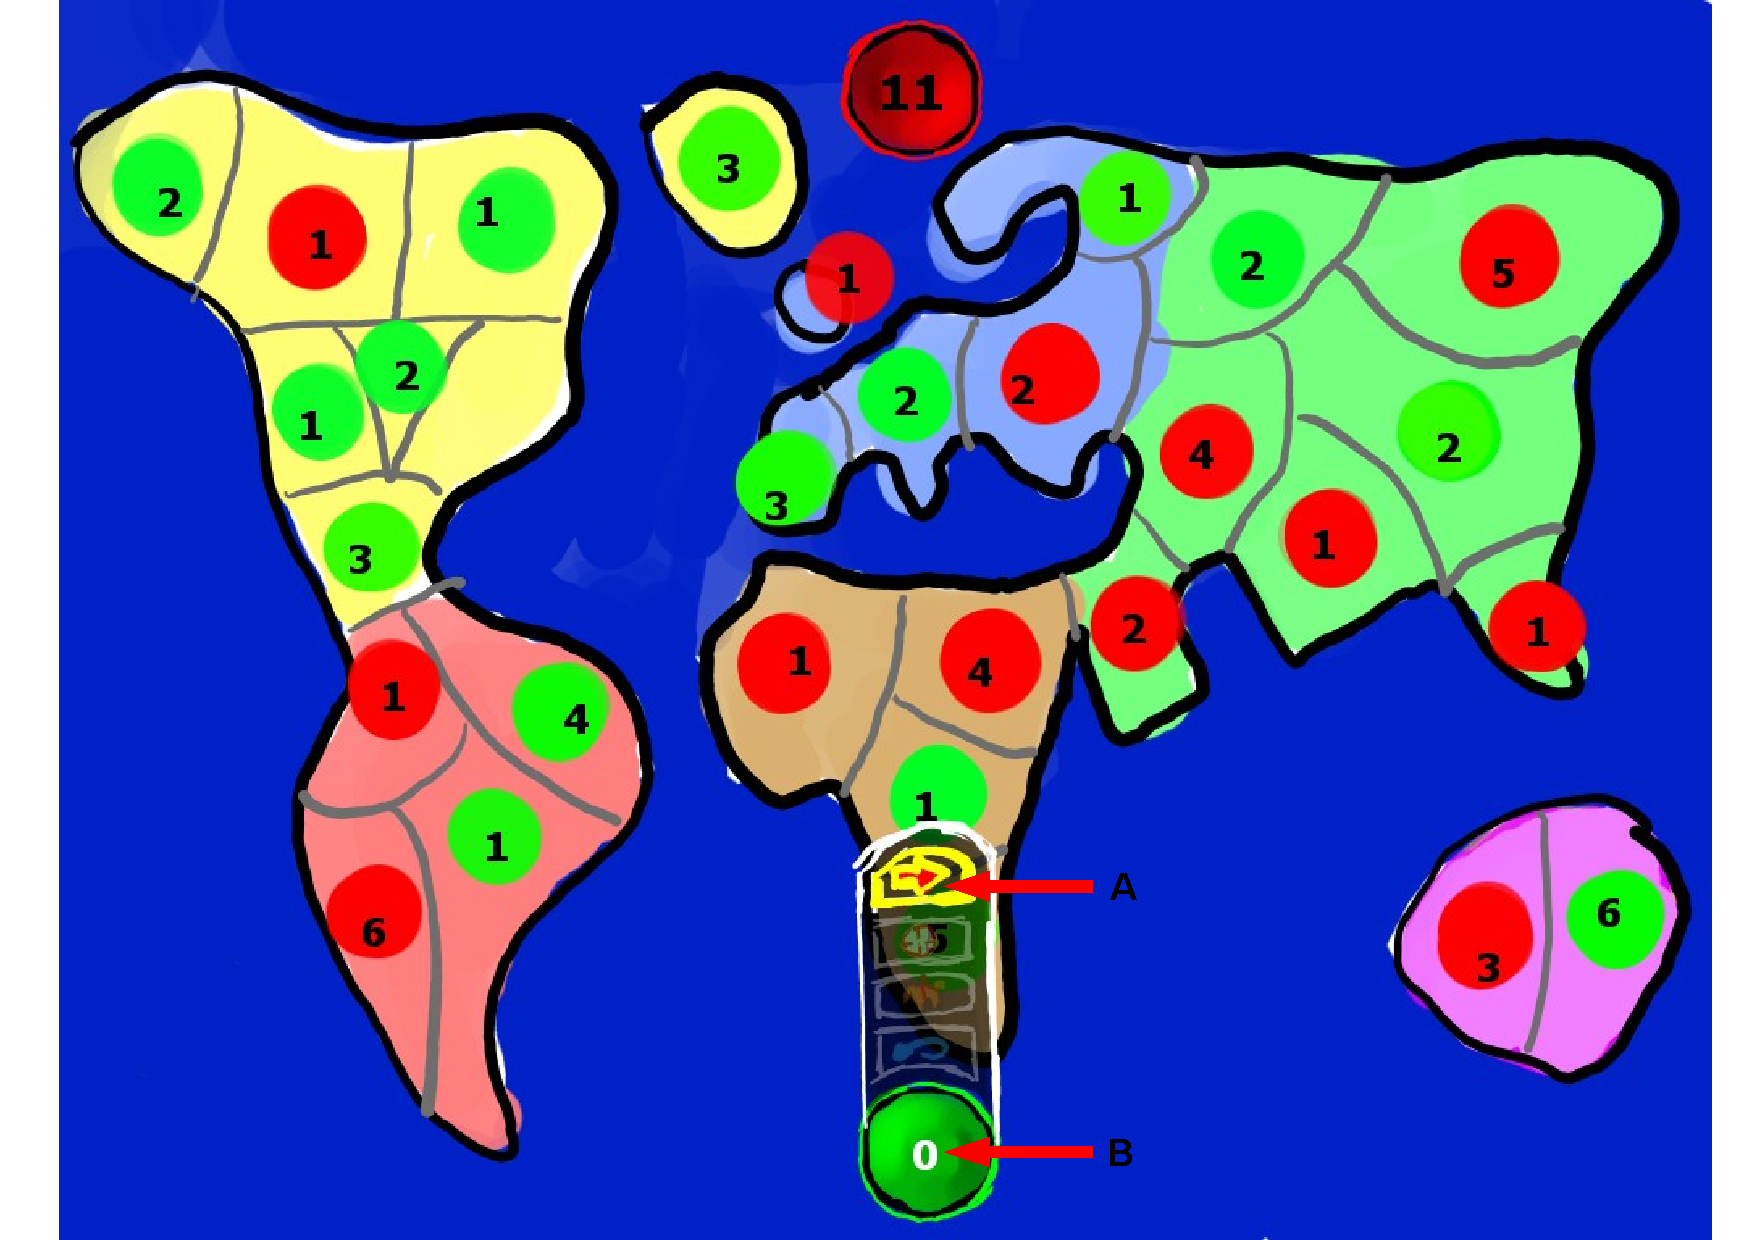
\includegraphics[width=11cm]{pic/mocks/3-6.pdf}
\end{figure}

\begin{table}[H]
\small
\centering
\begin{tabular}{c|p{5cm}|p{7cm}}
& Name & Action \\ \hline\hline
%%%
A
&Next button
&Finish init phase.
\\B
&Green region troops
&Activates next button when reaches 0.
\end{tabular}
\end{table}


\subsection{In-game menu}\label{mock:74}

\subsubsection{Showing in-game menu}\label{mock:741}

\begin{figure}[H]
  \centering
  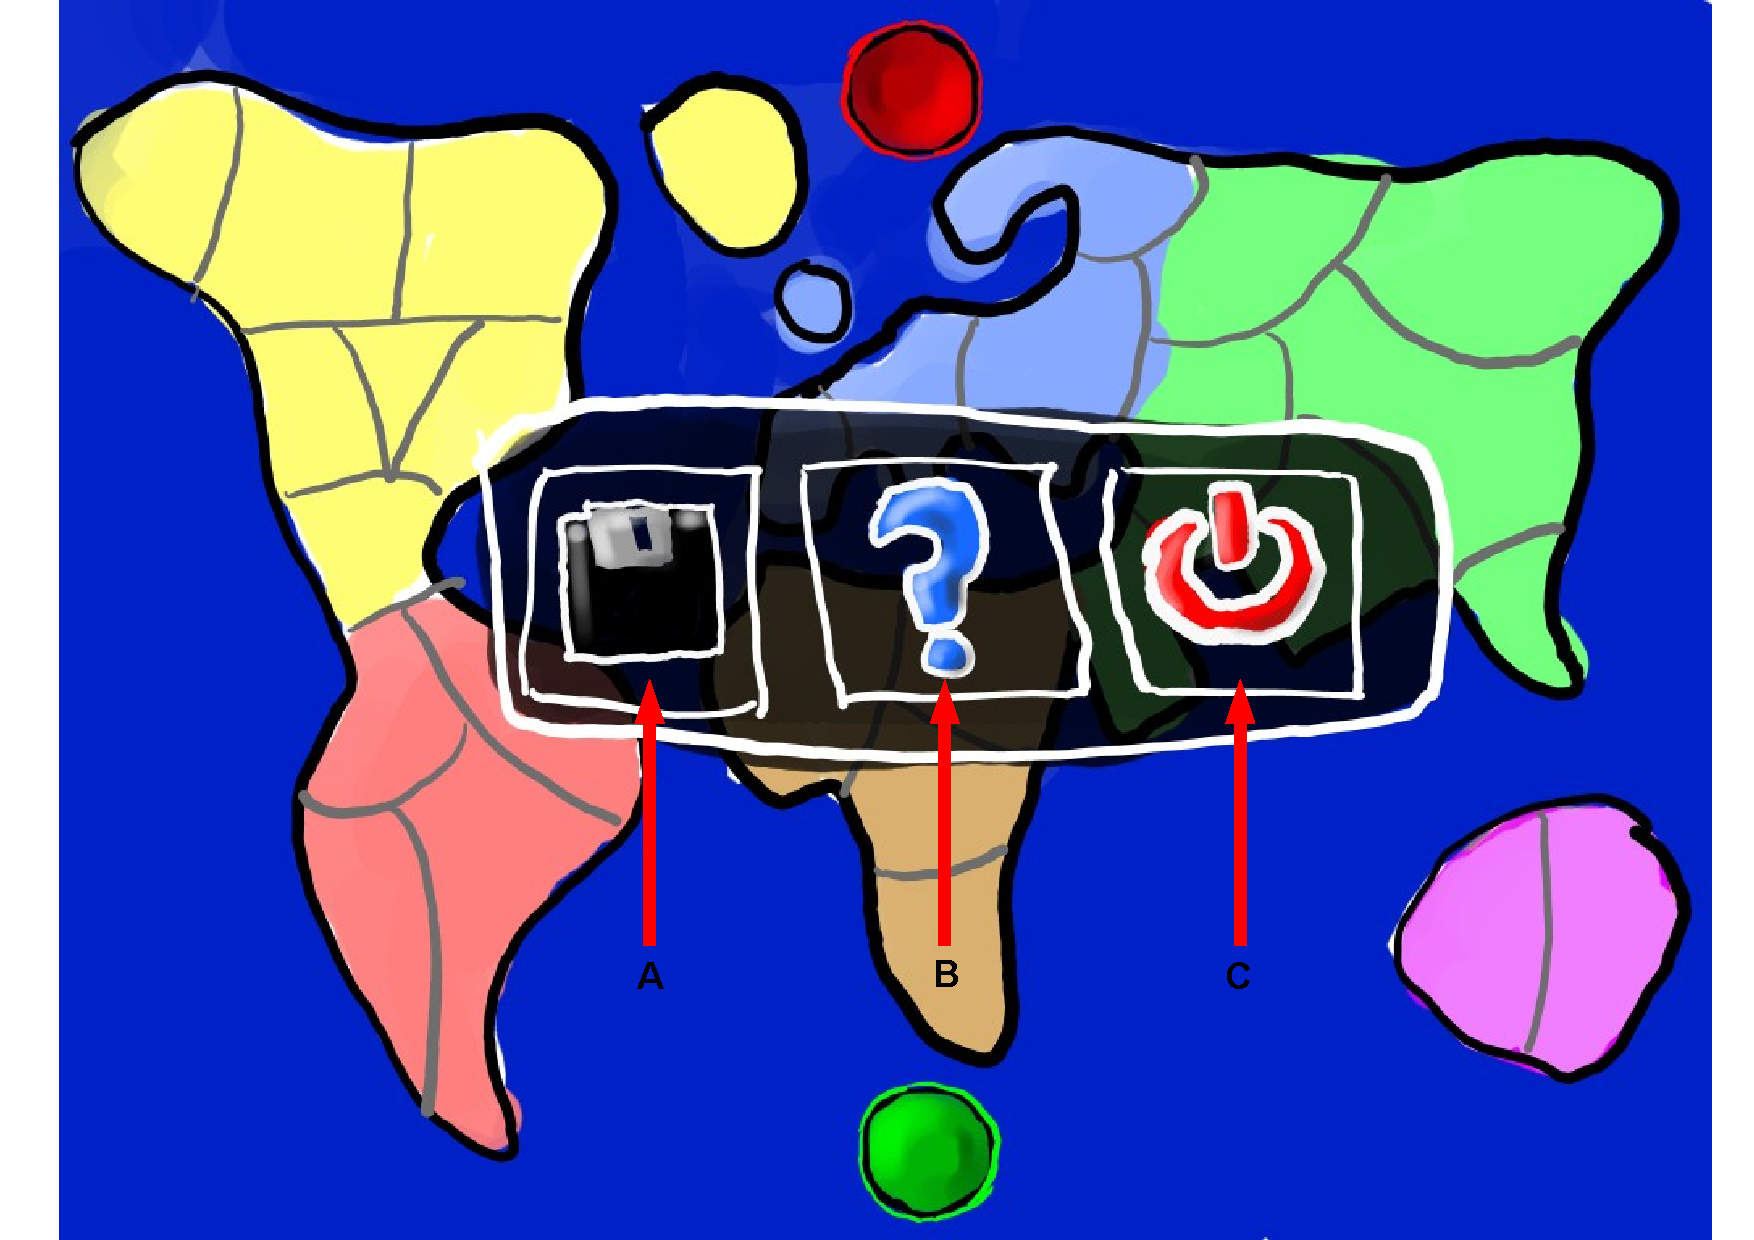
\includegraphics[width=11cm]{pic/mocks/4-1.pdf}
\end{figure}

\begin{table}[H]
\small
\centering
\begin{tabular}{c|p{5cm}|p{7cm}}
& Name & Action \\ \hline\hline
%%%
A
&Save
&Saves the game.
\\B
&Help
&Shows the help menu.
\\C
&Power
&Finish the game.
\end{tabular}
\end{table}

\subsection{Game Round}\label{mock:75}

\subsubsection{Reinforcements}\label{mock:751}

\begin{figure}[H]
  \centering
  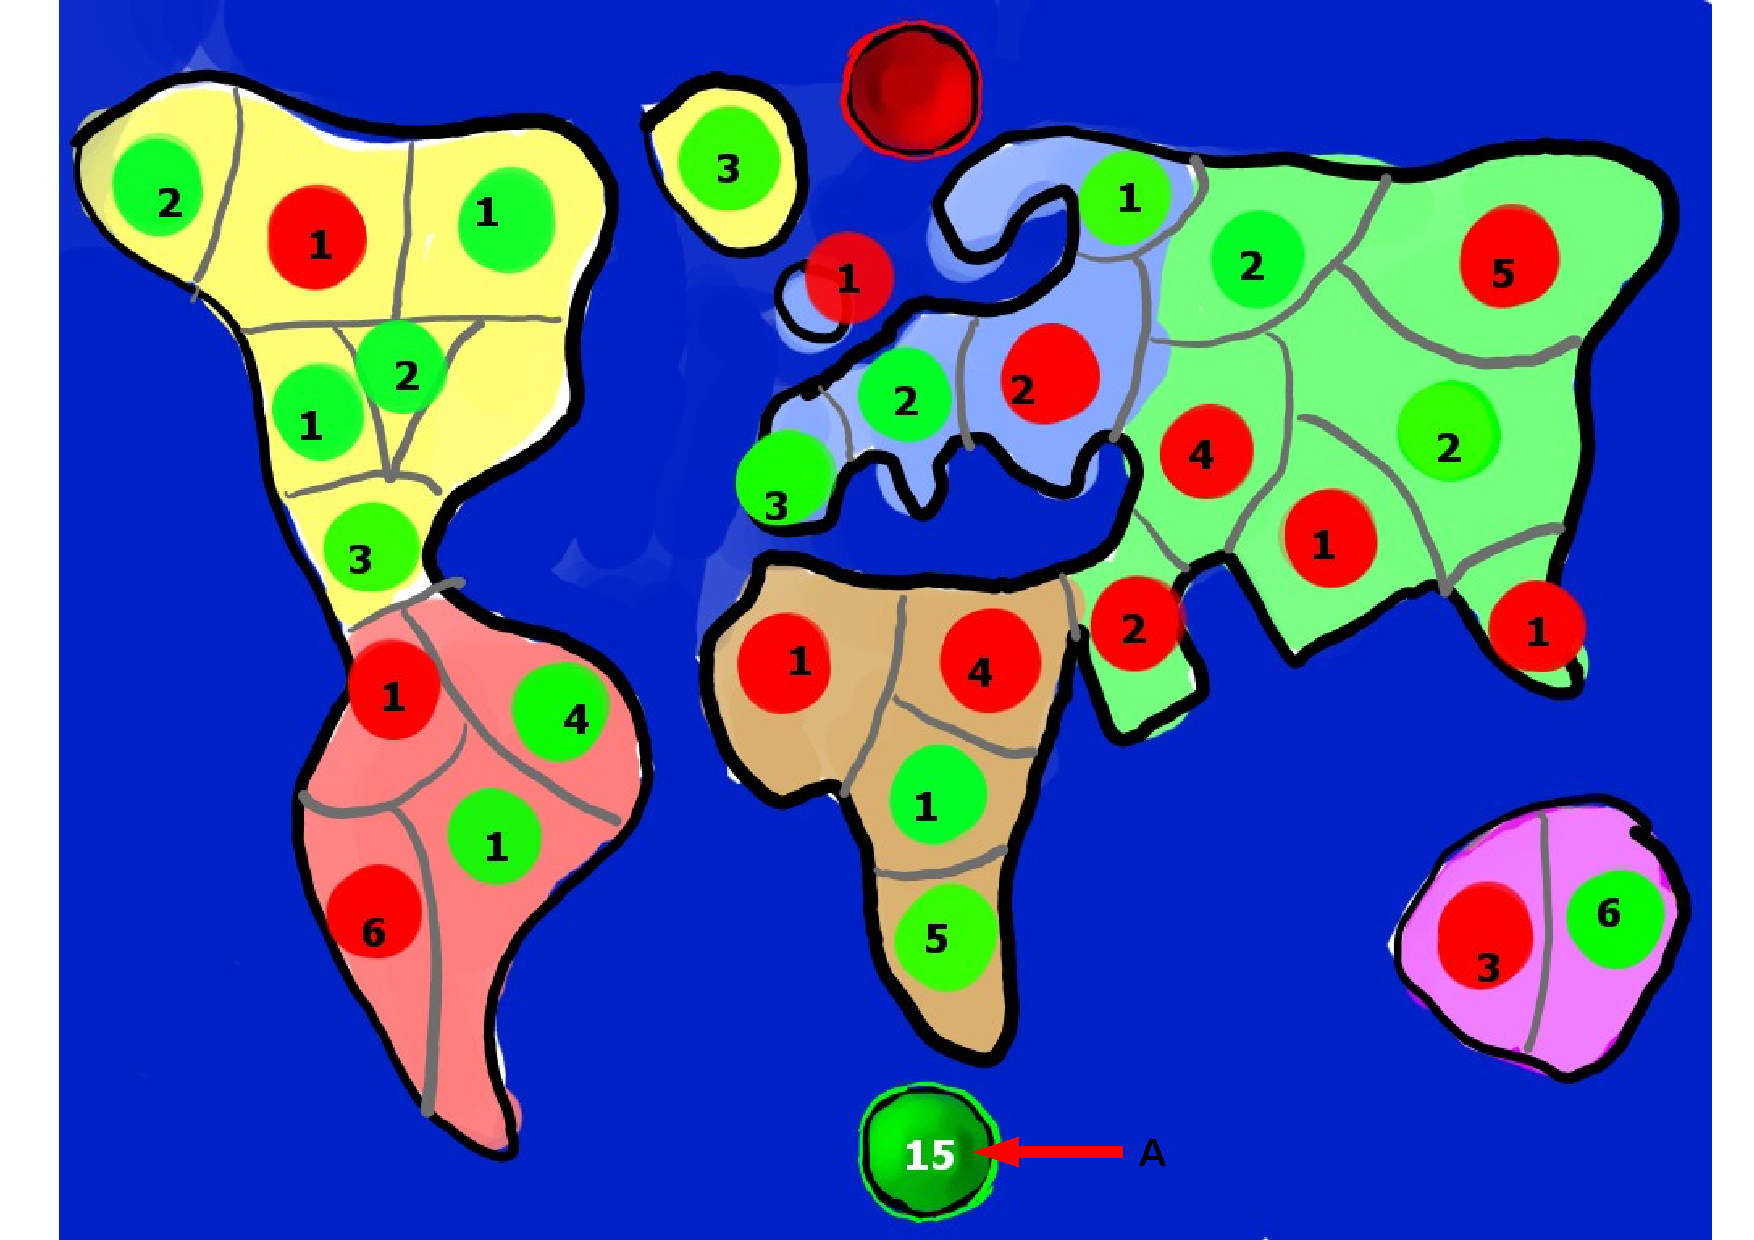
\includegraphics[width=11cm]{pic/mocks/5-1.pdf}
\end{figure}

\begin{table}[H]
\small
\centering
\begin{tabular}{c|p{5cm}|p{7cm}}
& Name & Action \\ \hline\hline
%%%
A
&Troops left
\end{tabular}
\end{table}

\subsubsection{Cards use}\label{mock:752}

\begin{figure}[H]
  \centering
  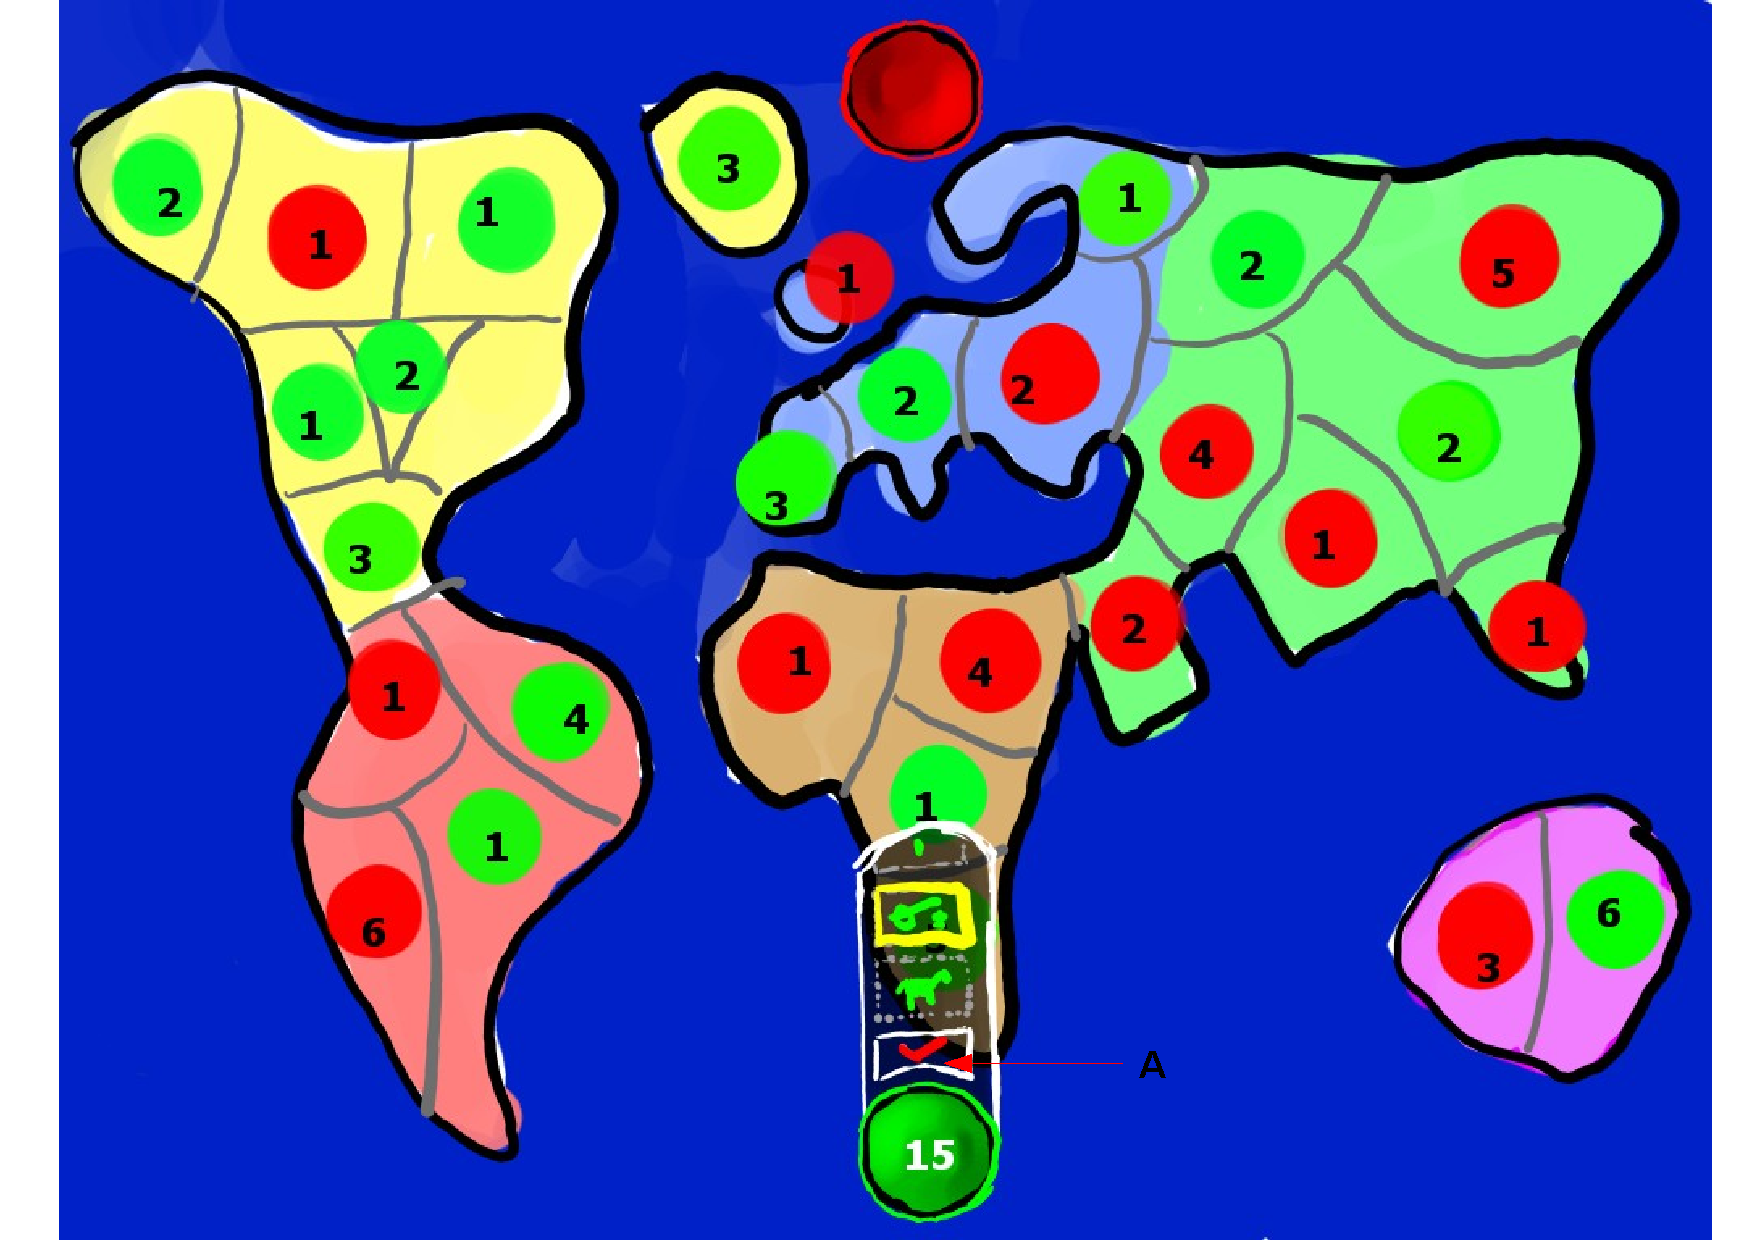
\includegraphics[width=11cm]{pic/mocks/5-2.pdf}
\end{figure}

\begin{table}[H]
\small
\centering
\begin{tabular}{c|p{5cm}|p{7cm}}
& Name & Action \\ \hline\hline
%%%
A
&Done button
&If the card selected make a valid combination, the result of troops is add to the number available.
\end{tabular}
\end{table}

\subsubsection{Attack phase}\label{mock:753}

\begin{figure}[H]
  \centering
  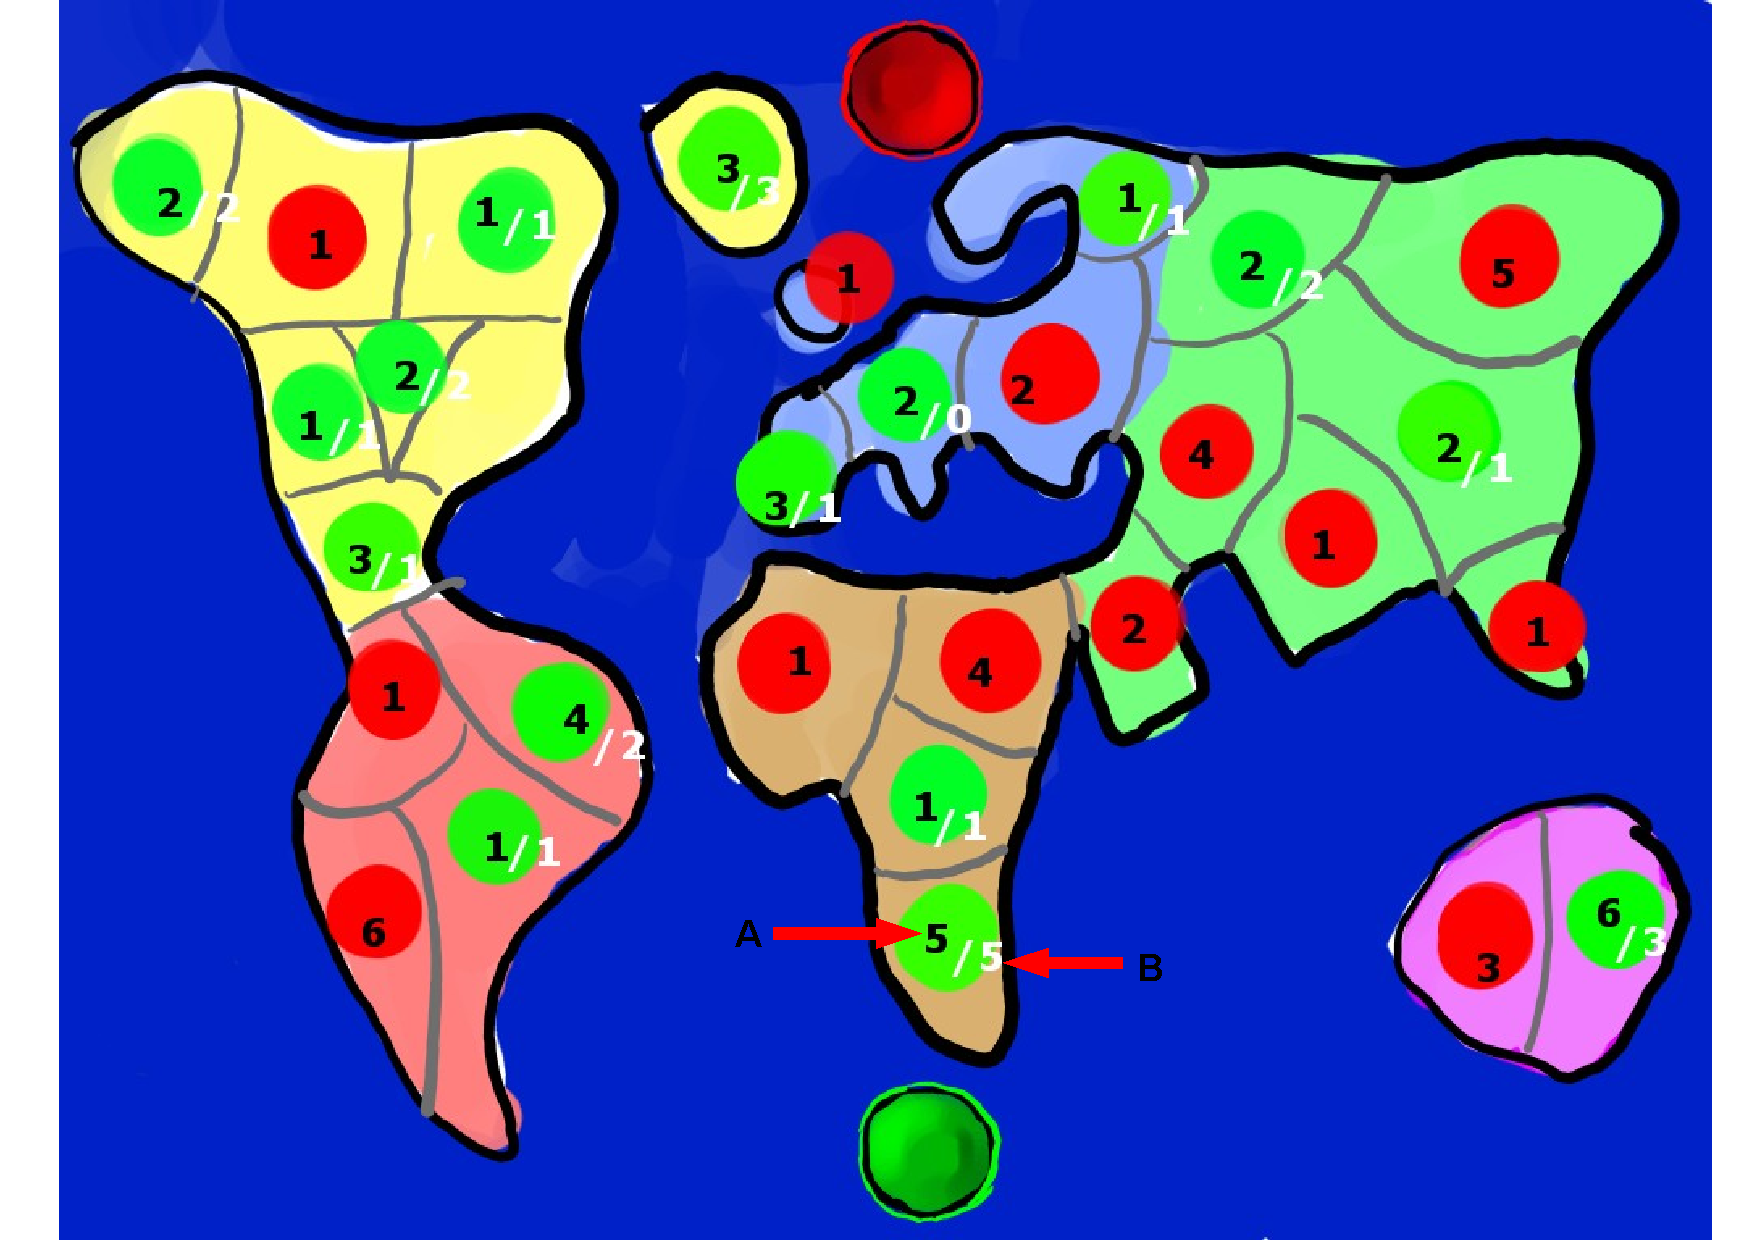
\includegraphics[width=11cm]{pic/mocks/5-3.pdf}
\end{figure}

\begin{table}[H]
\small
\centering
\begin{tabular}{c|p{5cm}|p{7cm}}
& Name & Action \\ \hline\hline
%%%
A
&Troops in region
\\B
&Troops available.
&Troops available to use in an attack.
\end{tabular}
\end{table}


\subsubsection{Attack phase - Region selected}\label{mock:754}

\begin{figure}[H]
  \centering
  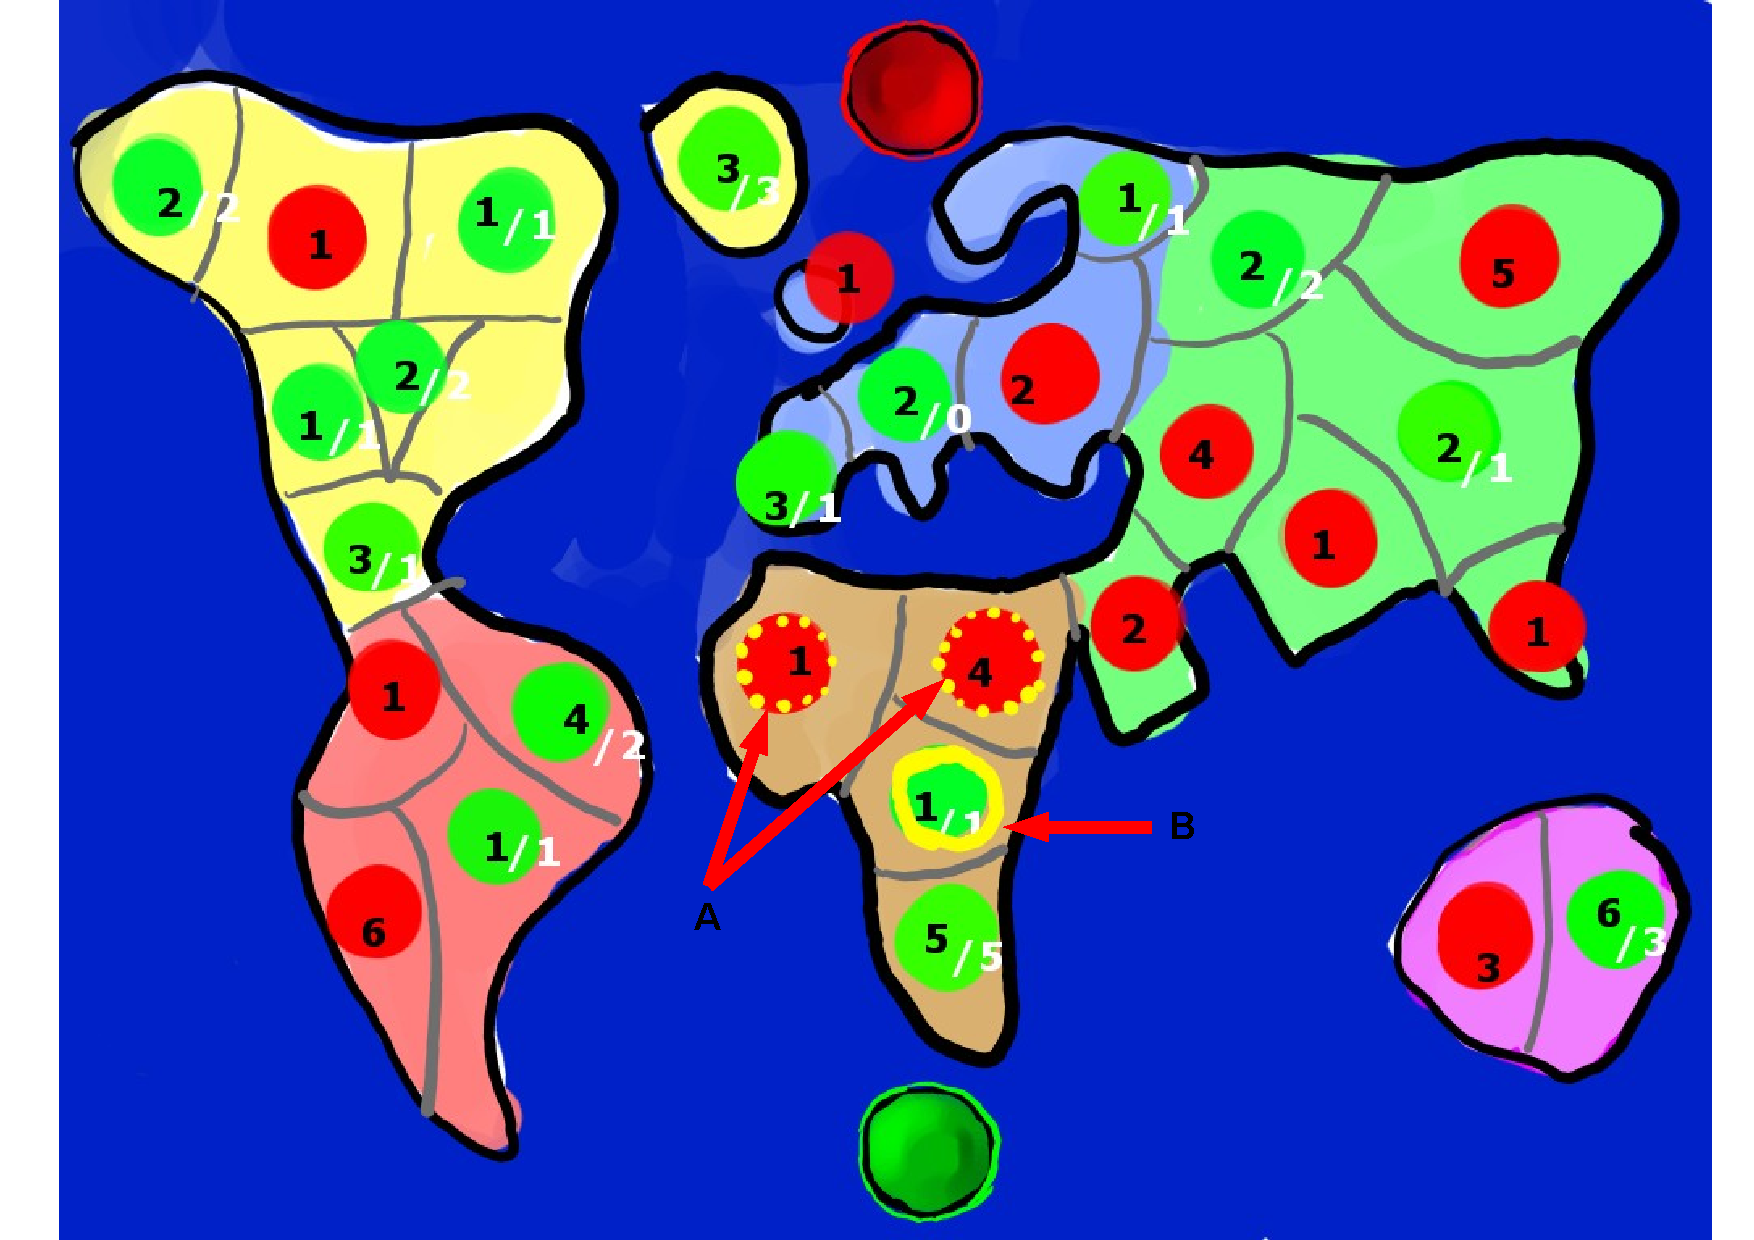
\includegraphics[width=11cm]{pic/mocks/5-4.pdf}
\end{figure}

\begin{table}[H]
\small
\centering
\begin{tabular}{c|p{5cm}|p{7cm}}
& Name & Action \\ \hline\hline
%%%
A
&Defenders
&Regions that are able to be attacked
\\B
&Attacker
&Region that is going to attack. Makes “Defenders” more visible when clicked.
\end{tabular}
\end{table}


\subsubsection{Movement phase}\label{mock:755}

\begin{figure}[H]
  \centering
  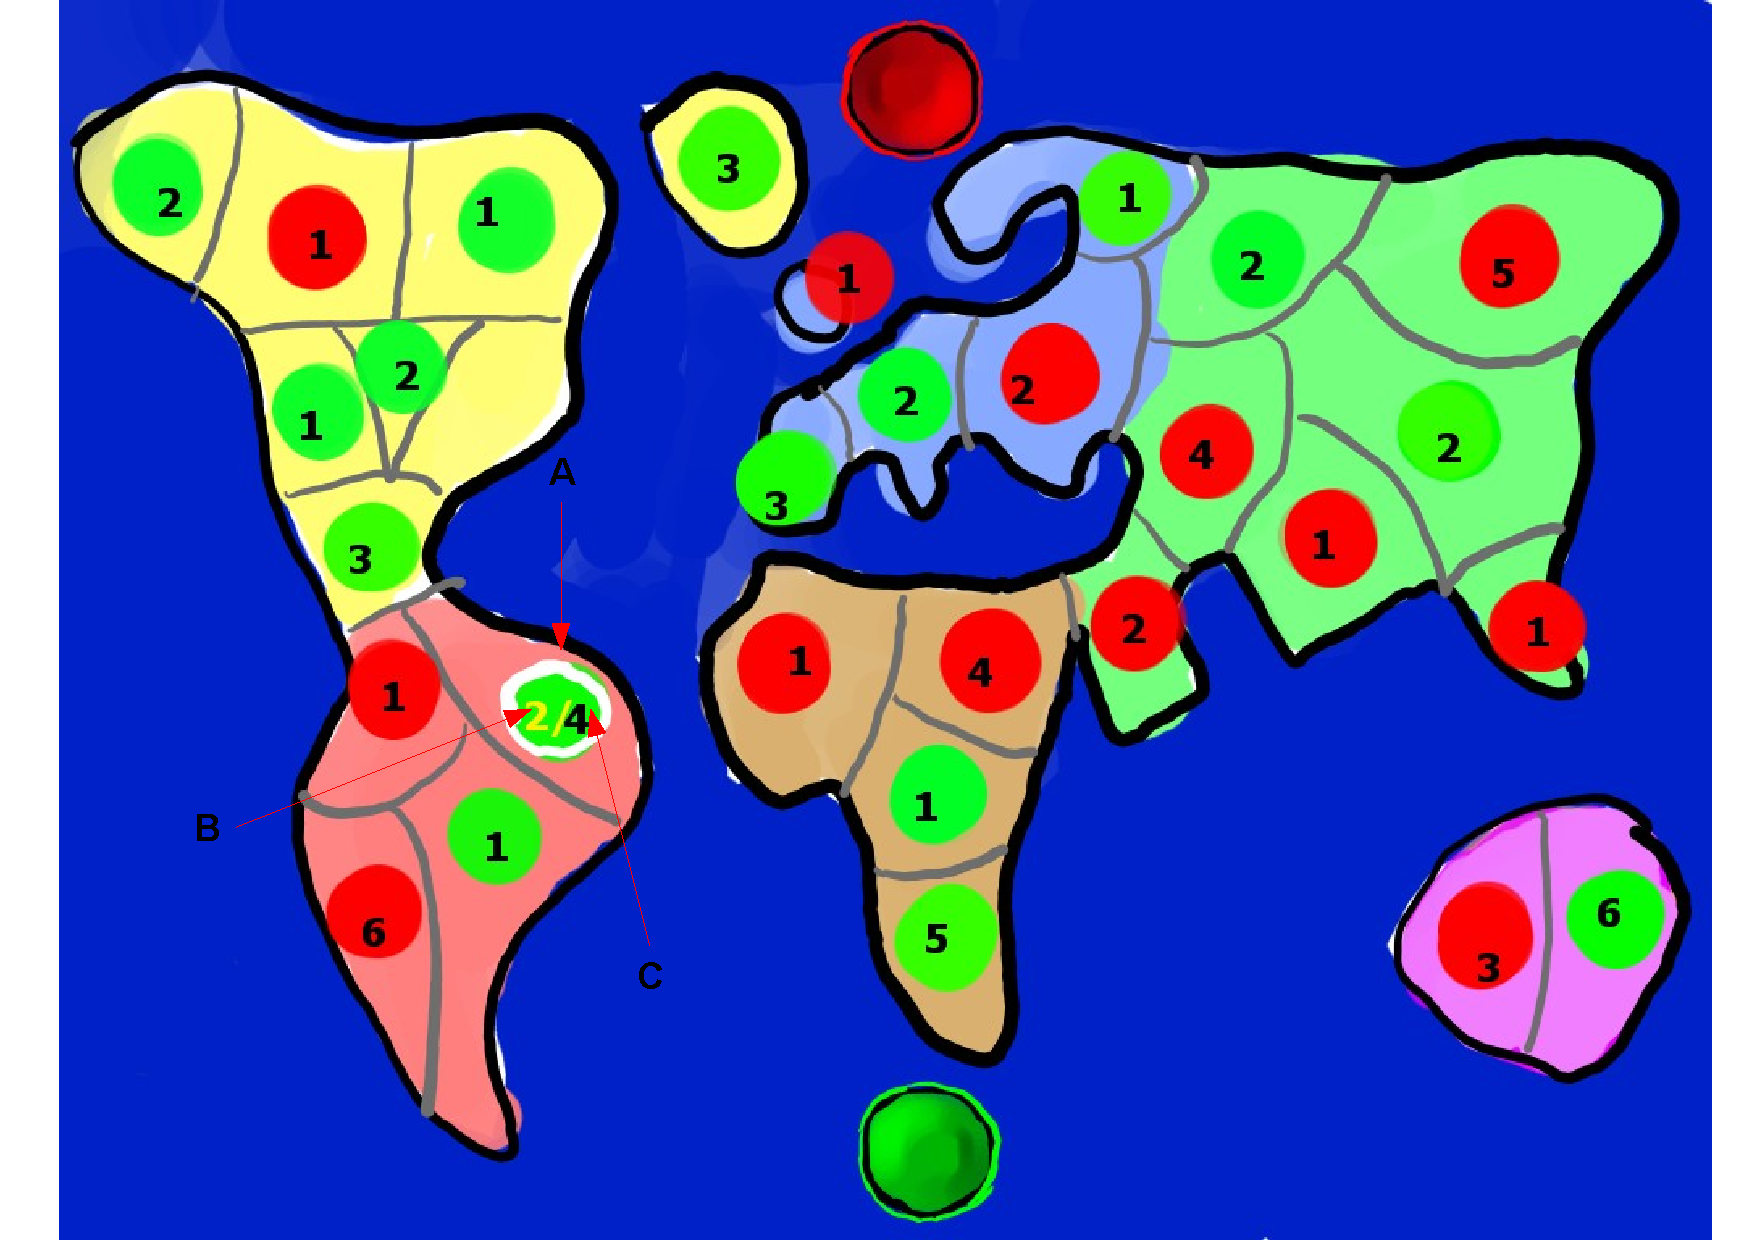
\includegraphics[width=11cm]{pic/mocks/5-5.pdf}
\end{figure}

\begin{table}[H]
\small
\centering
\begin{tabular}{c|p{5cm}|p{7cm}}
& Name & Action \\ \hline\hline
%%%
A
&Selected region
&
\\B
&Moveable units
&
\\C
&Total units
&
\end{tabular}
\end{table}


\subsection{Battle}\label{mock:76}

\subsubsection{Defender reinforcements}\label{mock:761}

\begin{figure}[H]
  \centering
  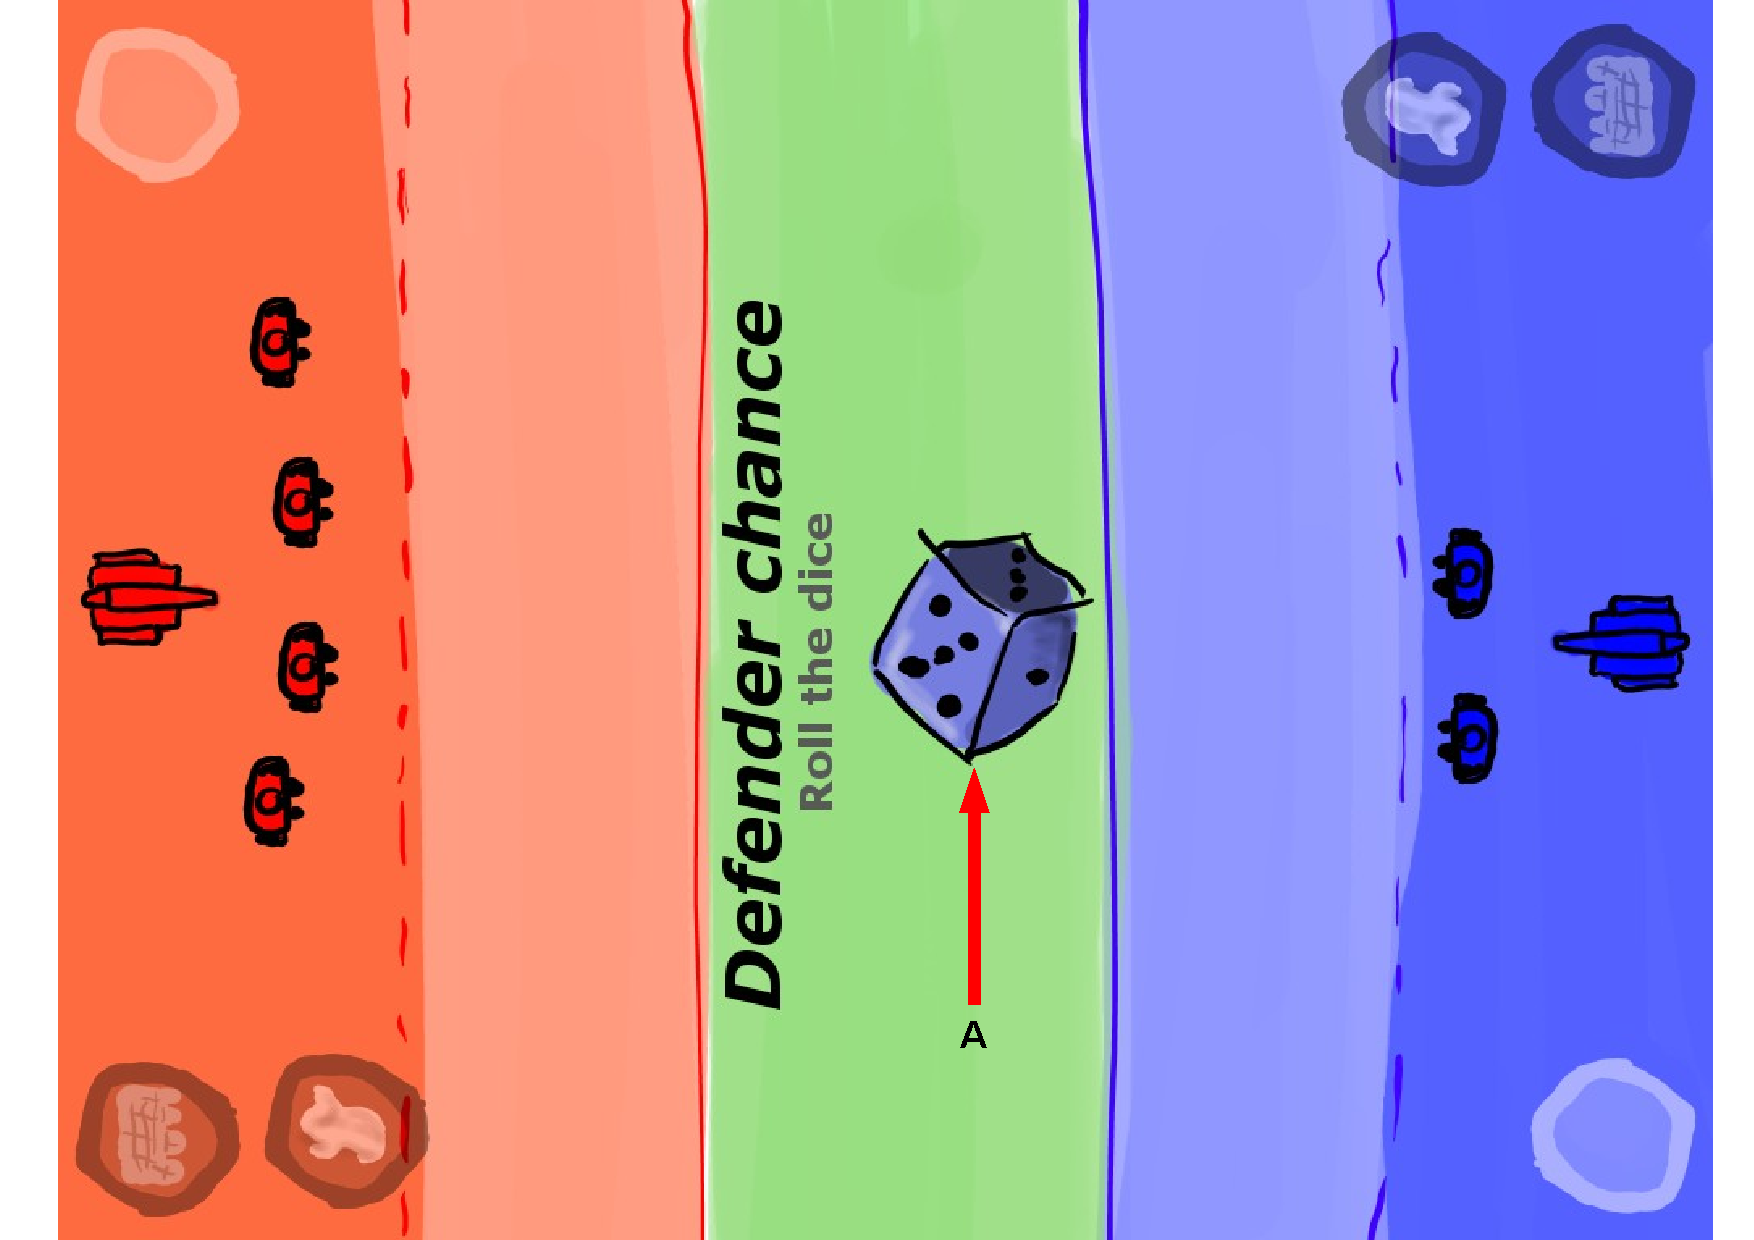
\includegraphics[width=11cm]{pic/mocks/6-1.pdf}
\end{figure}

\begin{table}[H]
\small
\centering
\begin{tabular}{c|p{5cm}|p{7cm}}
& Name & Action \\ \hline\hline
%%%
A
&Dice
&Roll when clicked.
\end{tabular}
\end{table}

\newpage
\subsubsection{Defender reinforcement ends}\label{mock:762}

\begin{figure}[H]
  \centering
  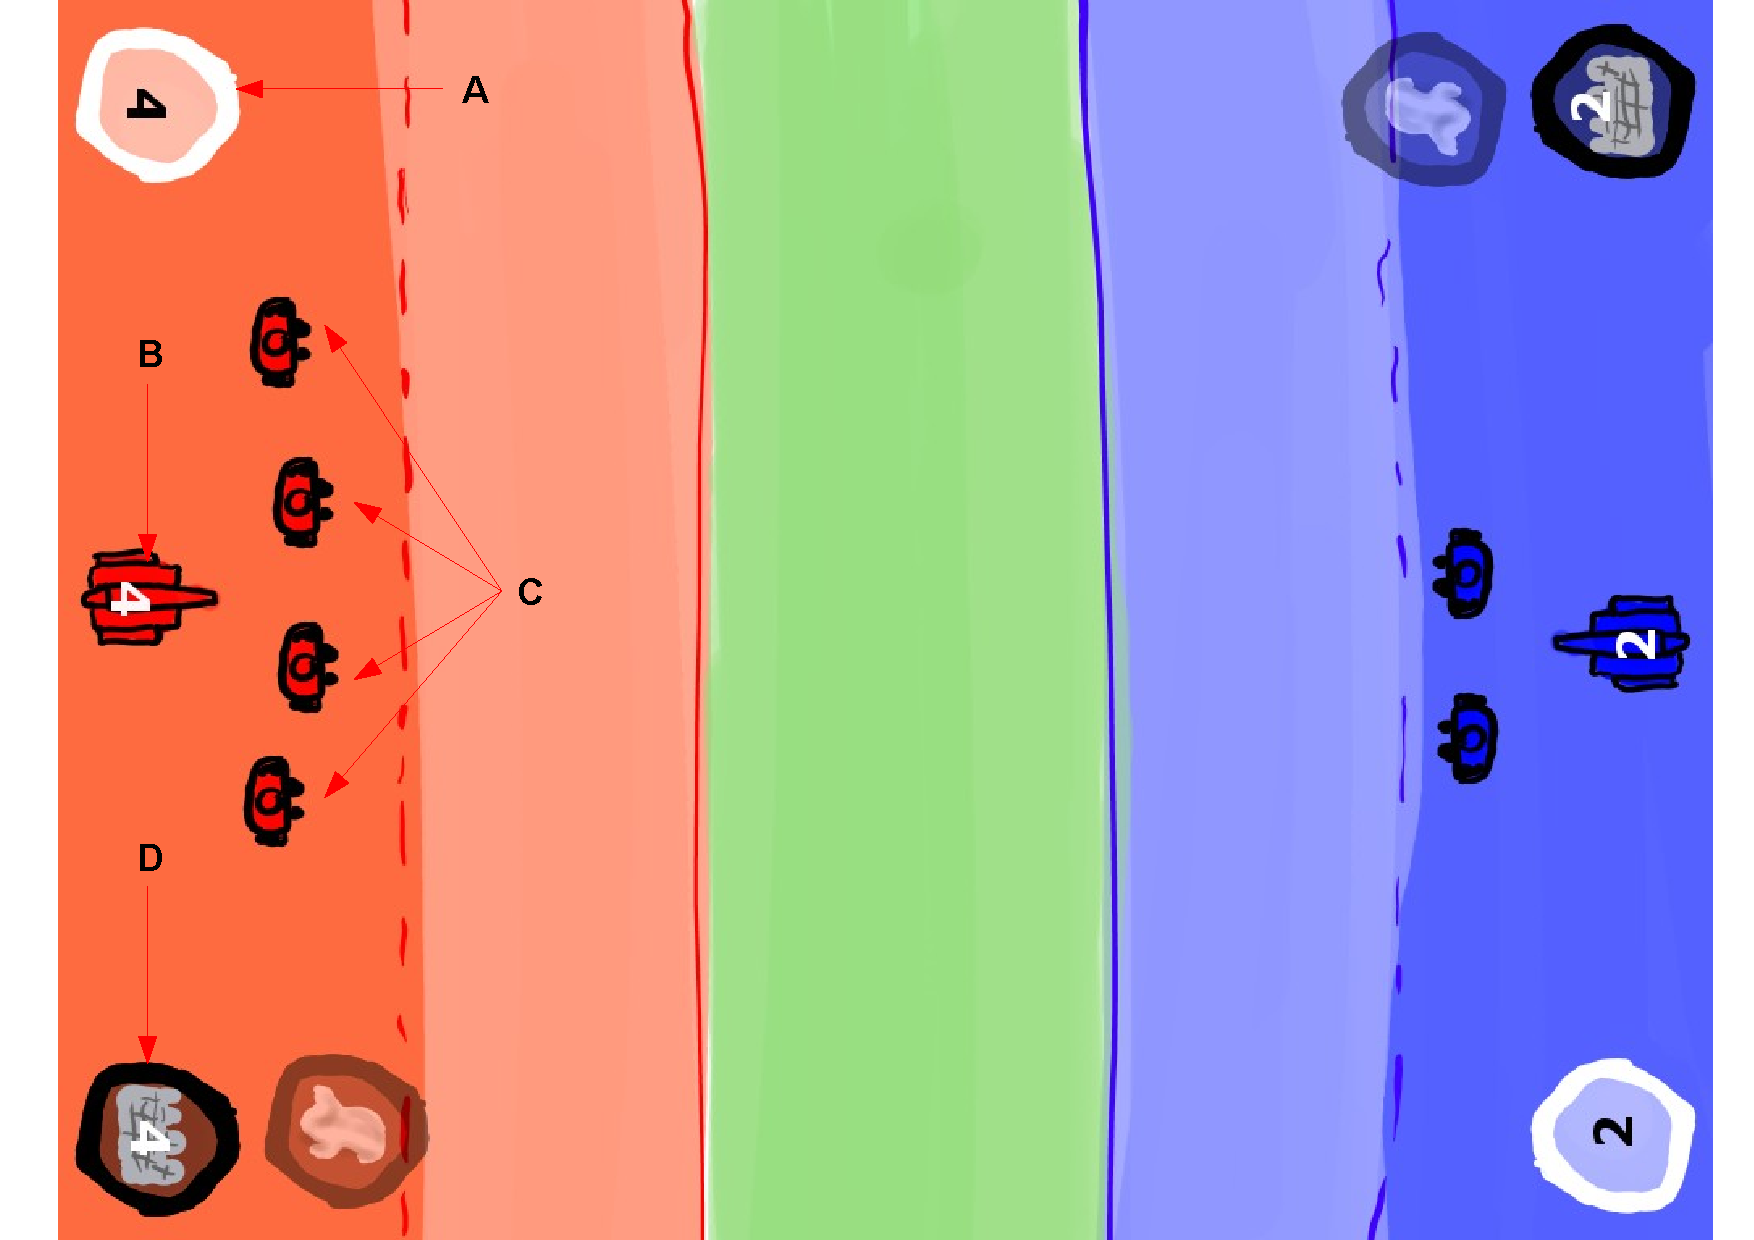
\includegraphics[width=11cm]{pic/mocks/6-2.pdf}
\end{figure}

\begin{table}[H]
\small
\centering
\begin{tabular}{c|p{5cm}|p{7cm}}
& Name & Action \\ \hline\hline
%%%
A
&Ready button
&Starts the battle after both players have clicked the button.
\end{tabular}
\end{table}

\newpage
\subsubsection{Battle starts}\label{mock:763}

\begin{figure}[H]
  \centering
  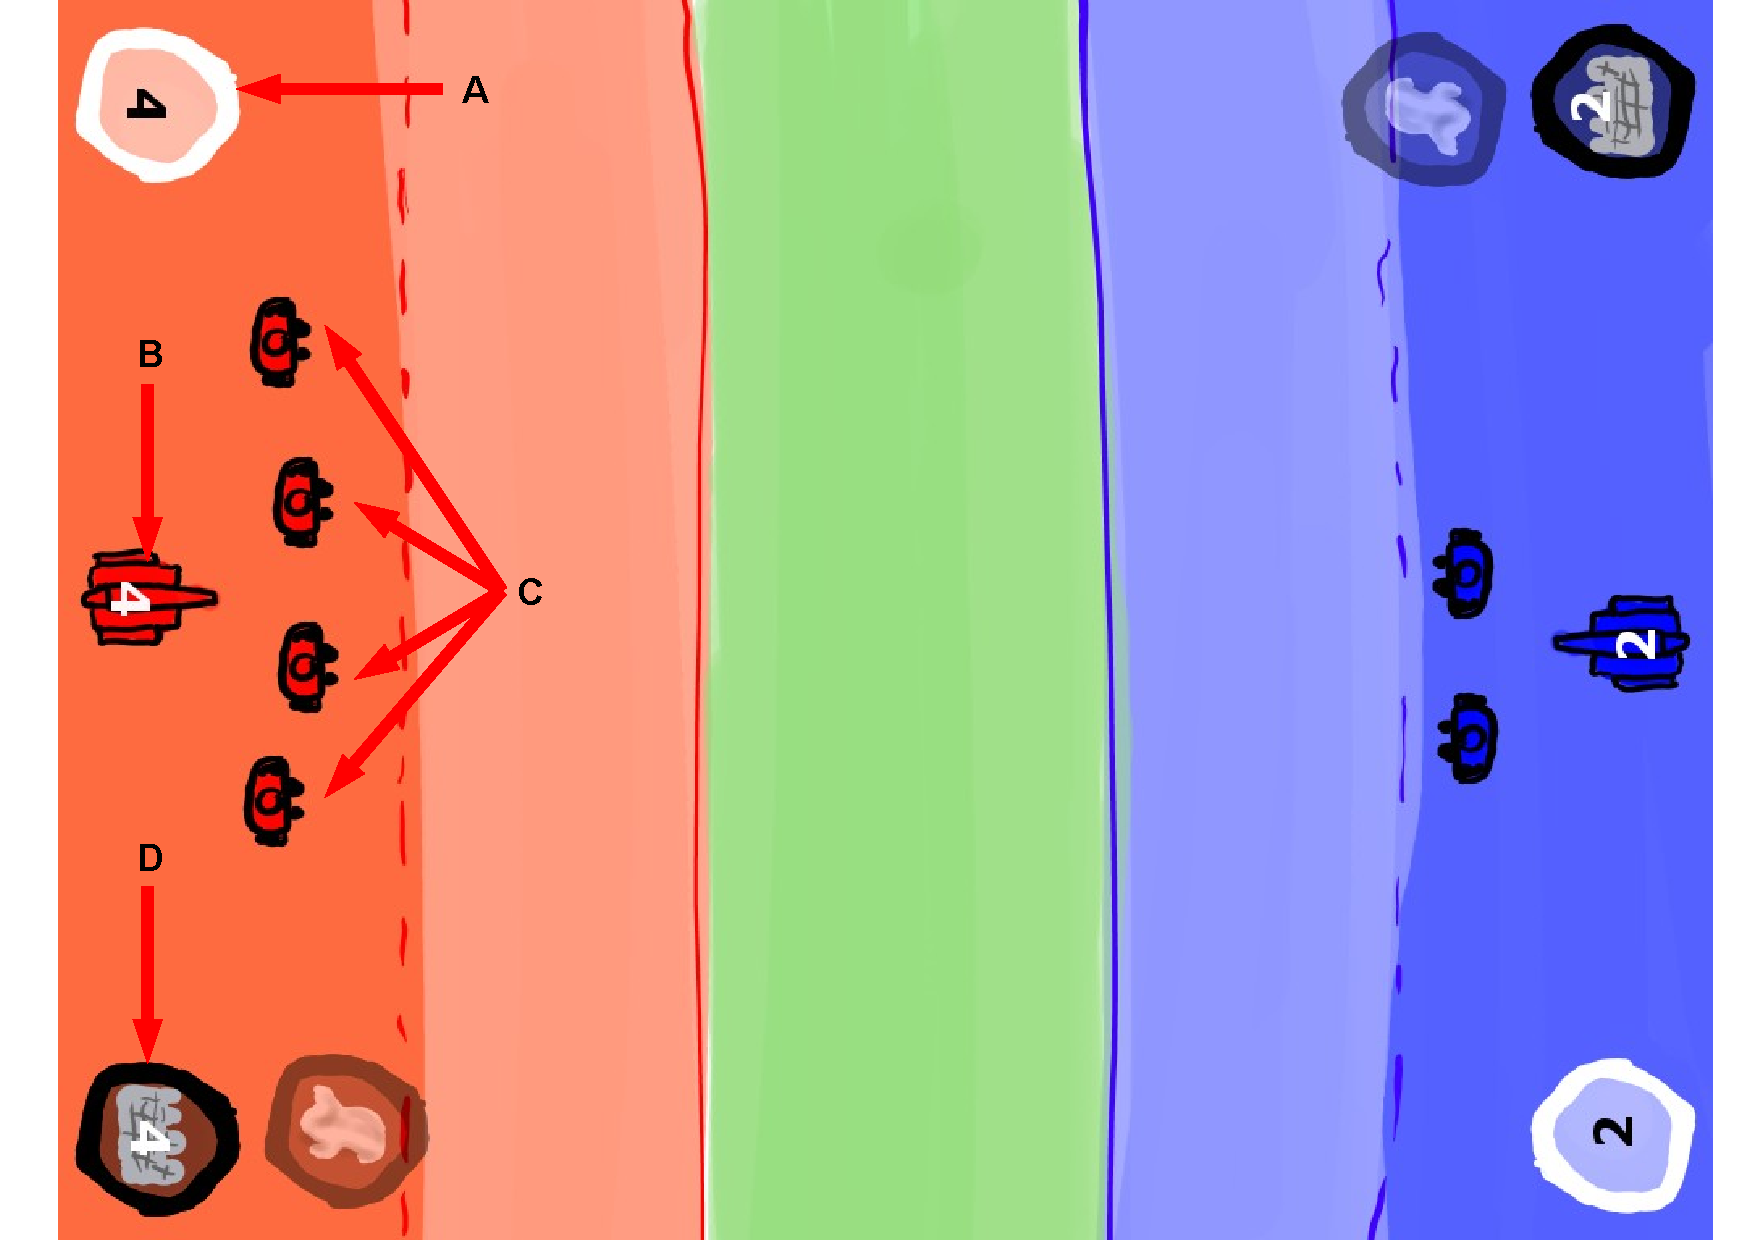
\includegraphics[width=11cm]{pic/mocks/6-3.pdf}
\end{figure}

\begin{table}[H]
\small
\centering
\begin{tabular}{c|p{5cm}|p{7cm}}
& Name & Action \\ \hline\hline
%%%
A
&
&
\\B
&Cannonballs available 
&Shoots cannon.
\\C
&Troops available
&Goes to \ref{mock:764}
\\D
&Walls available
&Goes to \ref{mock:766}
\end{tabular}
\end{table}


\subsubsection{Soldier movement}\label{mock:764}

\begin{figure}[H]
  \centering
  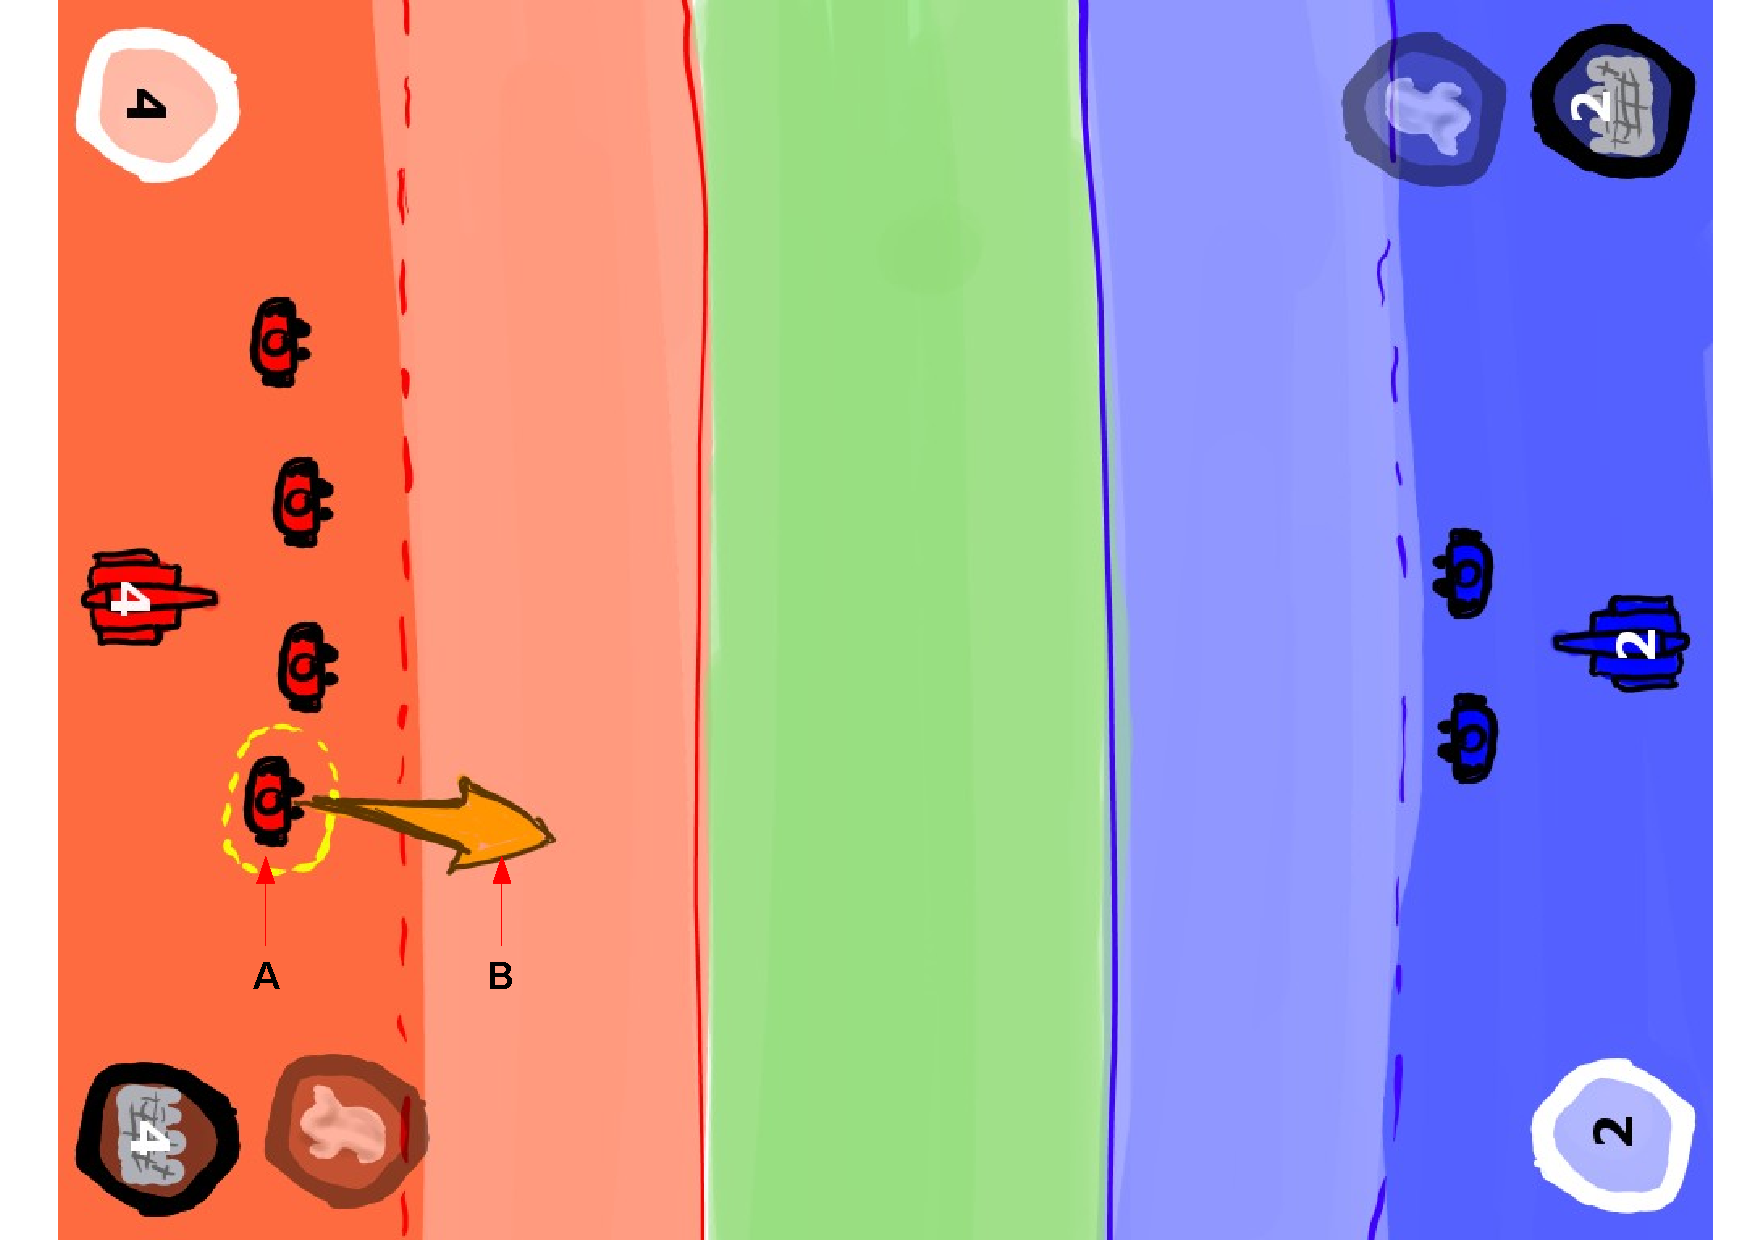
\includegraphics[width=11cm]{pic/mocks/6-4.pdf}
\end{figure}

\begin{table}[H]
\small
\centering
\begin{tabular}{c|p{5cm}|p{7cm}}
& Name & Action \\ \hline\hline
%%%
A
&Troop selected
&Shows direction arrow.
\\B
&Direction arrow 
&Moves the troop in the selected direction.
\end{tabular}
\end{table}


\newpage
\subsubsection{Retreat activates}\label{mock:765}
\begin{figure}[H]
  \centering
  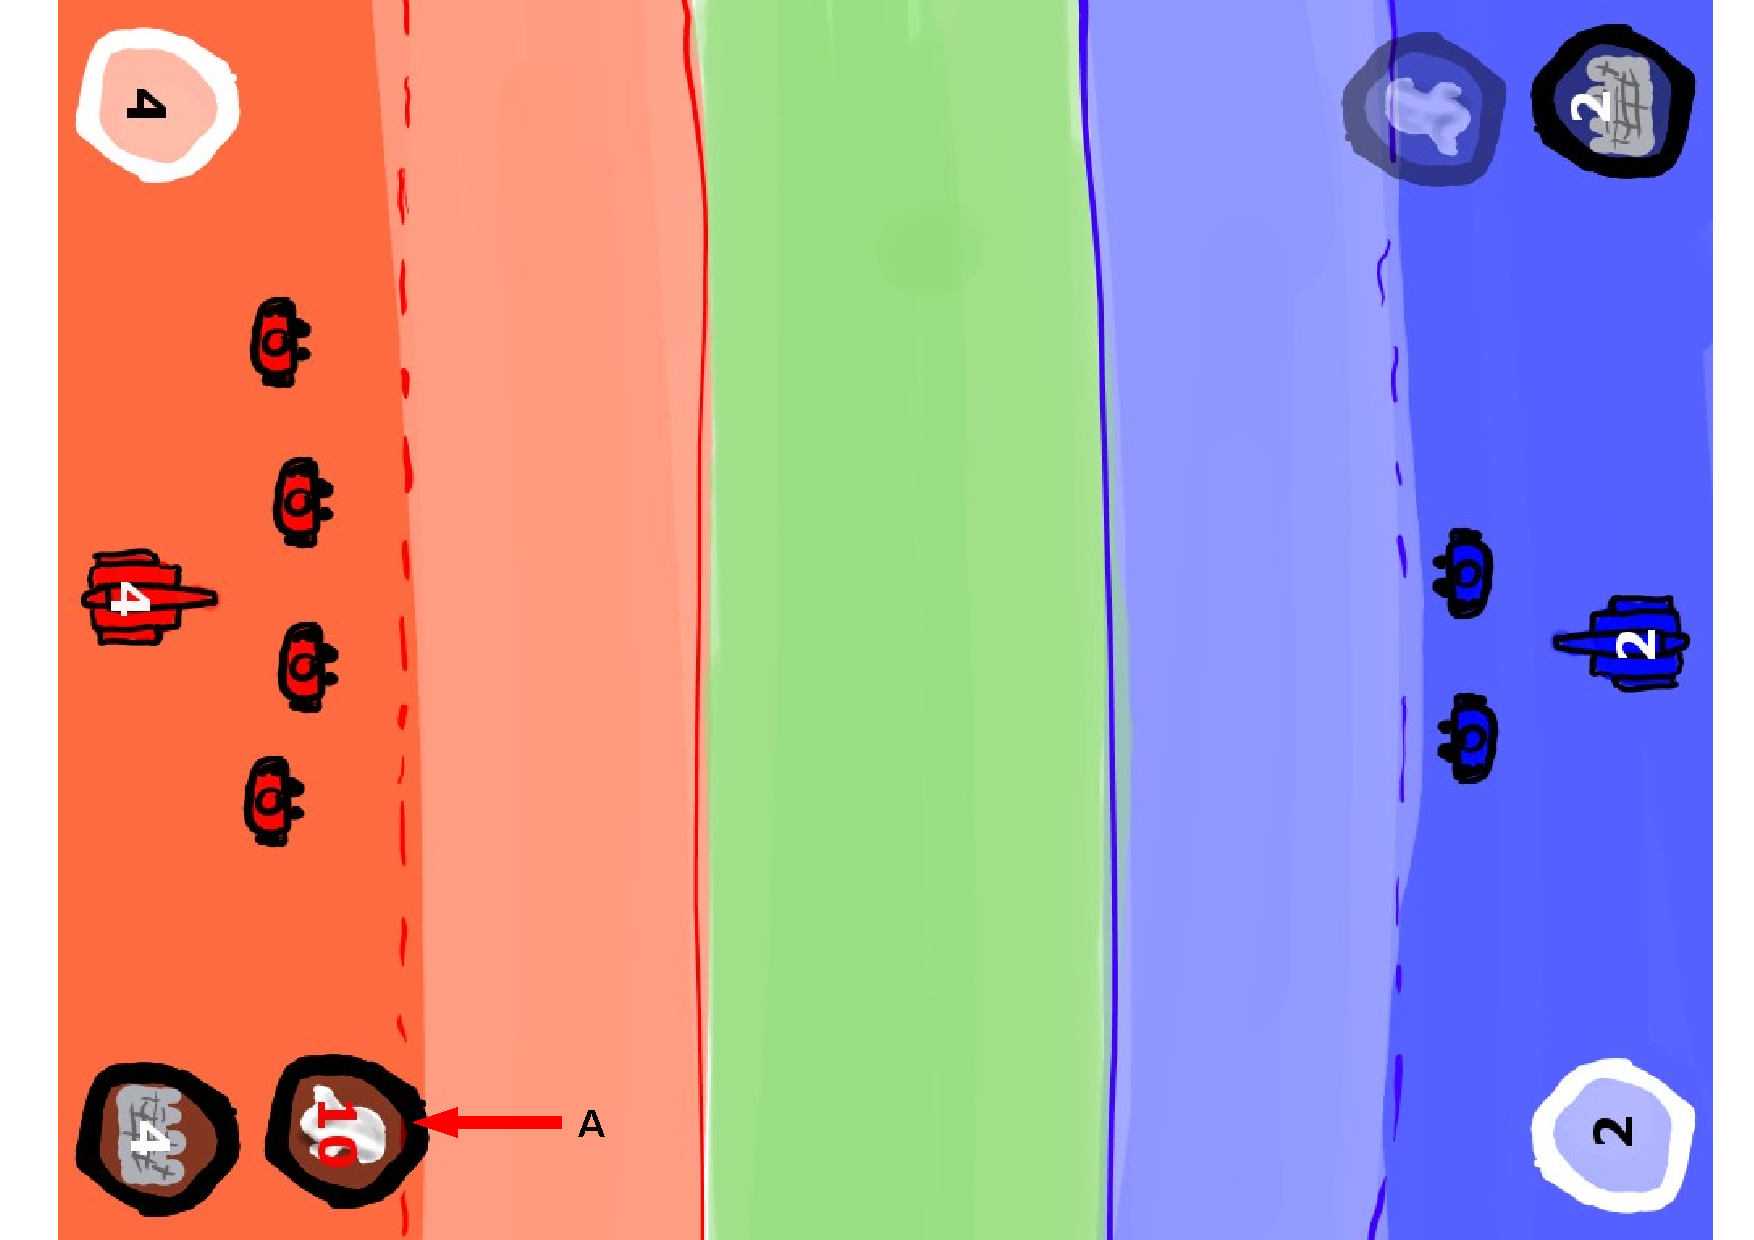
\includegraphics[width=11cm]{pic/mocks/6-5.pdf}
\end{figure}

\begin{table}[H]
\small
\centering
\begin{tabular}{c|p{5cm}|p{7cm}}
& Name & Action \\ \hline\hline
%%%
A
&Retreat countdown
&Retreats the attacker if clicked when available.
\end{tabular}
\end{table}

\newpage
\subsubsection{Wall placement}\label{mock:766}
\begin{figure}[H]
  \centering
  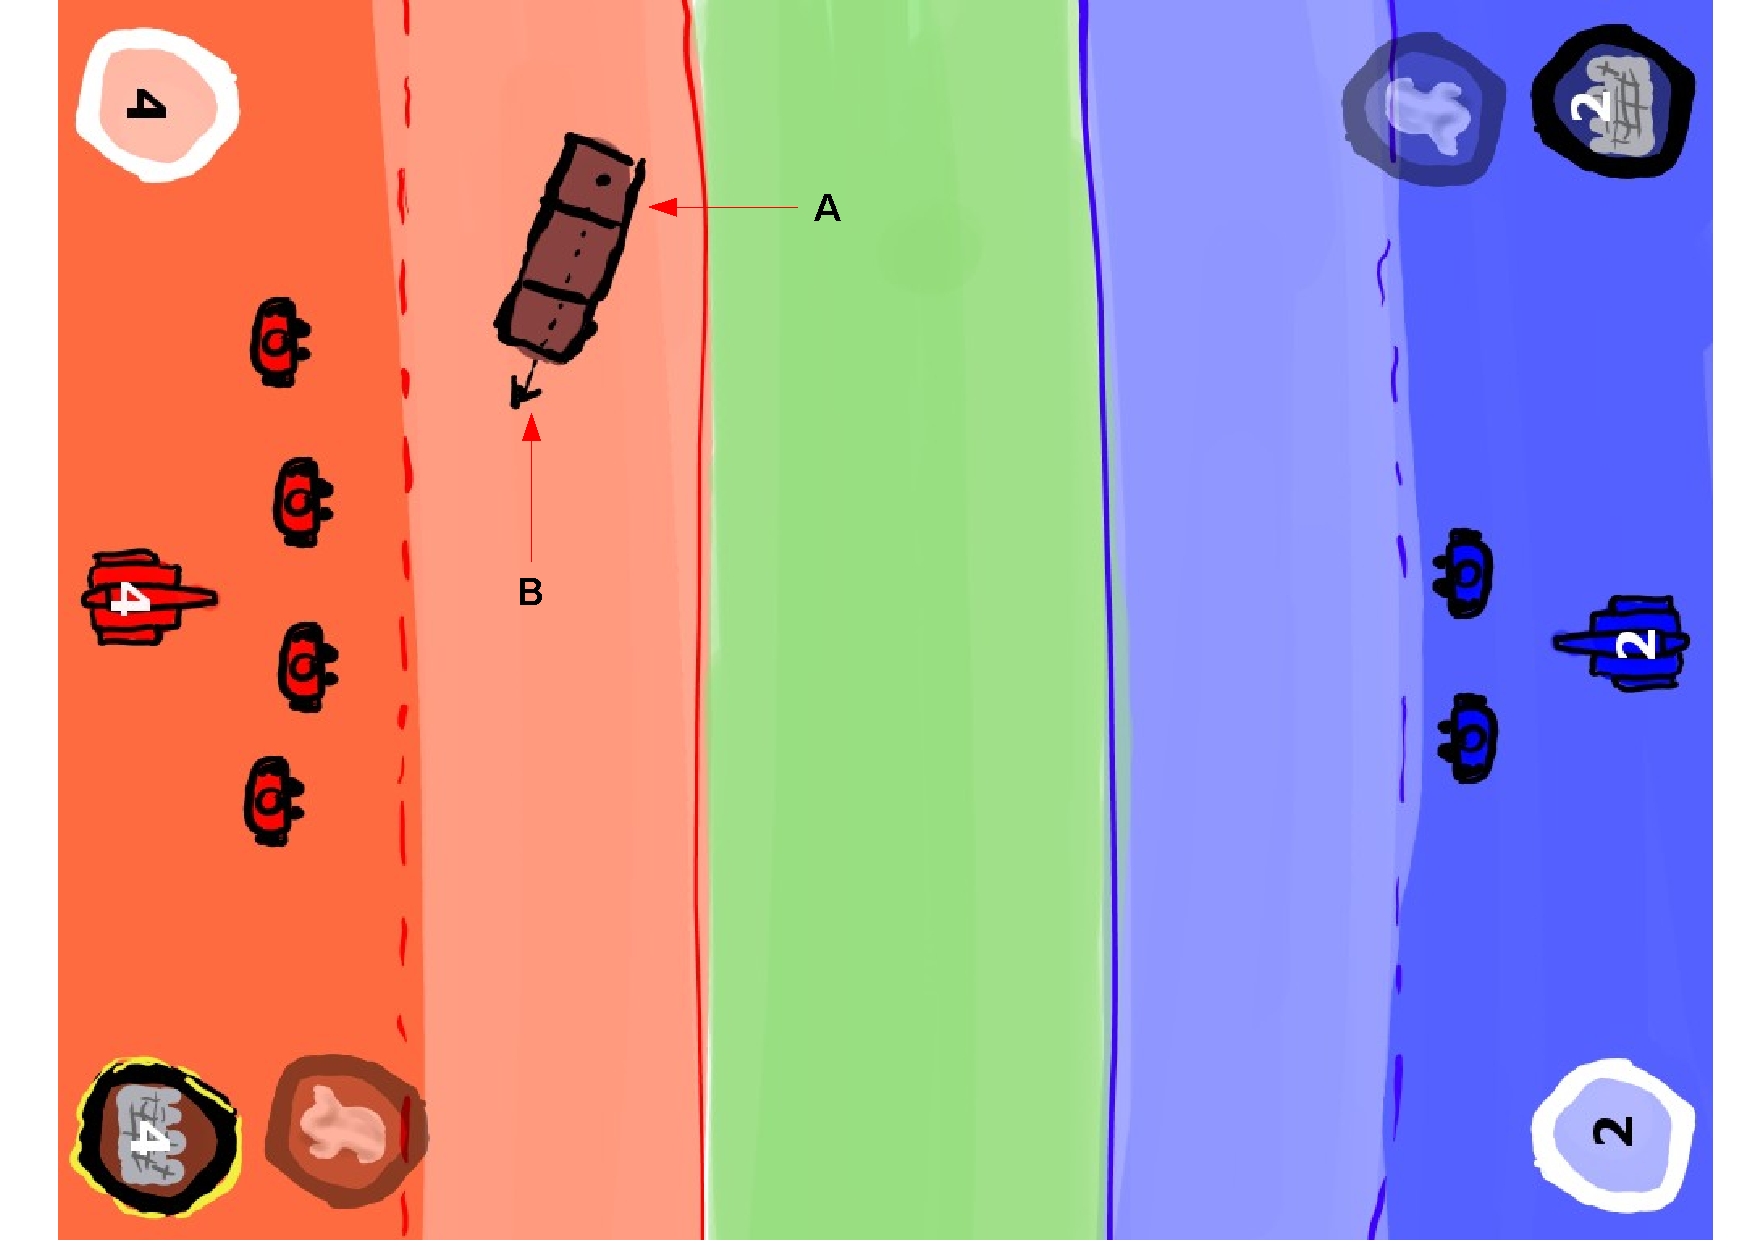
\includegraphics[width=11cm]{pic/mocks/6-6.pdf}
\end{figure}

\begin{table}[H]
\small
\centering
\begin{tabular}{c|p{5cm}|p{7cm}}
& Name & Action \\ \hline\hline
%%%
A
&Wall
&
\\B
&Wall direction
&Click and drag to place the wall.
\end{tabular}
\end{table}

\begin{todo}[Juan Pedro]
I see that there has been some misunderstandings between me (who draw
the mocks) and Alberto (who modelled the behaviour) and that the
intended behaviour of some parts of the mock-ups where not obvious. I
will try to fix it some other day :p
\end{todo}

\newpage
\startappendix

\end{document}
